% UW Thesis Template for LaTeX 
% Last Updated July 8, 2009 by Stephen Carr, IST Client Services
% FOR ASSISTANCE, please send mail to rt-IST-CSmathsci@ist.uwaterloo.ca

% Effective October 2006, the University of Waterloo 
% requires electronic thesis submission. See the UW thesis regulations at
% http://www.grad.uwaterloo.ca/Thesis_Regs/thesistofc.asp.
% However, many faculties/departments also require one or more printed
% copies. This template attempts to satisfy requirements for both types of output. 
% It is based on the standard "report" document class. The "book" document 
% class can be substituted if you have a very large, multi-part thesis.

% DISCLAIMER
% To the best of our knowledge, this template satisfies the current UW requirements.
% However, it is your responsibility to assure that you have met all 
% requirements of the University and your particular department.
% Many thanks to Colin Alie for assistance in preparing this updated template.

% -----------------------------------------------------------------------

% By default, output is produced that is geared toward generating a PDF 
% version optimized for viewing on an electronic display, including 
% hyperlinks within the PDF.
 
% E.g. to process a thesis called "mythesis.tex" based on this template, run:yea

% pdflatex mythesis	-- first pass of the pdflatex processor
% bibtex mythesis	-- generates bibliography from .bib data file(s) 
% pdflatex mythesis	-- fixes cross-references, bibliographic references, etc
% pdflatex mythesis	-- fixes cross-references, bibliographic references, etc

% If you use the recommended LaTeX editor, Texmaker, you would open the mythesis.tex
% file, then click the pdflatex button. Then run BibTeX (under the Tools menu).
% Then click the pdflatex button two more times. If you have an index as well,
% you'll need to run MakeIndex from the Tools menu as well, before running pdflatex
% the last two times.

% N.B. The "pdftex" program allows graphics in the following formats to be
% included with the "\includegraphics" command: PNG, PDF, JPEG, TIFF
% Tip 1: Generate your figures and photos in the size you want them to appear
% in your thesis, rather than scaling them with \includegraphics options.
% Tip 2: Any drawings you do should be in scalable vector graphic formats:
% SVG, PNG, WMF, EPS and then converted to PNG or PDF, so they are scalable in
% the final PDF as well.
% Tip 3: Photographs should be cropped and compressed so as not to be too large.

% To create a PDF output that is optimized for double-sided printing: 
%
% 1) comment-out the \documentclass statement in the preamble below, and
% un-comment the second \documentclass line.
%
% 2) change the value assigned below to the boolean variable
% "ElectronicVersion" from "true" to "false".

% --------------------- Start of Document Preamble -----------------------

% Specify the document class, default style attributes, and page dimensions
% For hyperlinked PDF, suitable for viewing on a computer, use this:
\documentclass[letterpaper,12pt,titlepage,oneside,final]{report}
 
% For un-hyperlinked PDF, suitable for double-sided printing, use this:
%\documentclass[letterpaper,12pt,titlepage,openright,twoside,final]{report}

% Some LaTeX commands I define for my own nomenclature.
% If you have to, it's better to change nomenclature once here than in a 
% million places throughout your thesis!
\newcommand{\package}[1]{\textbf{#1}} % package names in bold text
\newcommand{\cmmd}[1]{\textbackslash\texttt{#1}} % command name in tt font 
\newcommand{\href}[1]{#1} % does nothing, but defines the command so the
    % print-optimized version will ignore \href tags (redefined by hyperref pkg).
%\newcommand{\texorpdfstring}[2]{#1} % does nothing, but defines the command
% Anything defined here may be redefined by packages added below...

% This package allows if-then-else control structures.
\usepackage{ifthen}
\newboolean{ElectronicVersion}
\setboolean{ElectronicVersion}{true} % CHANGE THIS VALUE AS REQUIRED

%\usepackage{nomencl} % For a nomenclature (optional; available from ctan.org)
\usepackage{amsmath,amssymb,amstext} % Lots of math symbols and environments
\usepackage[pdftex]{graphicx} % For including graphics N.B. pdftex graphics driver 
\usepackage[bindingoffset=0.125in,centering,includeheadfoot,margin=1in]{geometry}
\usepackage{algorithm}
\usepackage{algorithmic}
\usepackage{subfigure}
\usepackage{multirow}
\usepackage{lscape}
\usepackage{amstext}
\usepackage{easymat}
\usepackage{amsmath}
\usepackage{amssymb}
\usepackage{calc}
\usepackage{longtable}
%\usepackage{times}
%\usepackage{cmr}
\usepackage{setspace}
\usepackage{listings}
\usepackage{graphicx}
\usepackage{textcomp}
\usepackage{latexsym}
\usepackage{geometry}

\newtheorem{theorem}{Theorem}[section]
\newtheorem{lemma}[theorem]{Lemma}
\newtheorem{proposition}[theorem]{Proposition}
\newtheorem{corollary}[theorem]{Corollary}

\newenvironment{proof}[1][Proof]{\begin{trivlist}
\item[\hskip \labelsep {\bfseries #1}]}{\end{trivlist}}
\newenvironment{definition}[1][Definition]{\begin{trivlist}
\item[\hskip \labelsep {\bfseries #1}]}{\end{trivlist}}
\newenvironment{example}[1][Example]{\begin{trivlist}
\item[\hskip \labelsep {\bfseries #1}]}{\end{trivlist}}
\newenvironment{remark}[1][Remark]{\begin{trivlist}
\item[\hskip \labelsep {\bfseries #1}]}{\end{trivlist}}
\newcommand{\maj}{\ensuremath{\operatorname{maj}}}


% Hyperlinks make it very easy to navigate an electronic document.
% The following statement places "bookmarks" in the PDF document
% linking Table of Contents, List of Figures, List of Tables, and
% List of References entries to their appearance in the body of the
% text.  In addition, this is where one would specify the thesis title
% and author as they appear in the properties of the PDF document.

% Use the "hyperref" package only for the electronic version:
% N.B. HYPERREF MUST BE THE LAST PACKAGE LOADED; ADD ADDITIONAL PKGS ABOVE
\ifthenelse{\boolean{ElectronicVersion}}{
    \usepackage[letterpaper=true,pdftex,bookmarks,pagebackref,
	plainpages=false, % Needed if Roman numbers in frontpages
        pdfpagelabels=true, % Adds page number as label in Acrobat's page count 
        pdftitle=Combinatorial and Probabilistic Approaches to Motif-Recognition, % CHANGE THIS TEXT!
        pdfauthor=Christina\ Anne\ Boucher	 % CHANGE THIS TEXT!
        ]{hyperref}}{}

% Setting up the page margins...
% UW thesis requirements specify a minimum of 1 inch (72pt) margin at the
% top, bottom, and outside page edges and a 1.125 inch (81pt) gutter
% margin (on binding side). While this is not an issue for electronic
% viewing, a PDF may be printed, and so we have the same page layout for
% both printed and electronic versions, we leave the gutter margin in.
% The standard method of setting margins is with the \setlength command.
% We have used the "geometry" package, added above, to do it in one line.
% For completeness, the appropriate \setlength commands are show here, 
% commented out.
% Set margins to minimum permitted by UW thesis regulations:
%\setlength{\marginparwidth}{0pt} % width of margin notes
% N.B. If margin notes are used, you must adjust \textwidth, \marginparwidth
% and \marginparsep so that the space left between the margin notes and page
% edge is less than 15 mm (0.6 in.)
%\setlength{\marginparsep}{0pt} % width of space between body text and margin notes
%\setlength{\evensidemargin}{0.5in} % Adds 1/8 in. to binding side of all 
% even-numbered pages when the "twoside" printing option is selected
%\setlength{\oddsidemargin}{0.5in} % Adds 1/8 in. to the left of all pages
% when "oneside" printing is selected, and to the left of all odd-numbered
% pages when "twoside" printing is selected
%\setlength{\textwidth}{6.0in} % assuming US letter paper (8.5 in. x 11 in.) and 
% side margins as above
\raggedbottom

% The following statement specifies the amount of space between
% paragraphs. Other reasonable specifications are \bigskipamount and \smallskipamount.
\setlength{\parskip}{\medskipamount}

% The following statement controls the line spacing.  The default
% spacing corresponds to good typographic conventions and only slight
% changes (e.g., perhaps "1.2"), if any, should be made.
\renewcommand{\baselinestretch}{1} % this is the default line space setting

% By default, each chapter will start on a recto (right-hand side)
% page. We also force each section of the front pages to start on 
% a recto page by inserting \cleardoublepage commands in the 
% uw-ethesis-frontpgs.tex file, included below, with the \input command.
% In many cases, this will require that the verso page be
% blank and, while it should be counted, a page number should not be
% printed.  The following statements ensure a page number is not
% printed on an otherwise blank verso page.
\let\origdoublepage\cleardoublepage
\newcommand{\clearemptydoublepage}{%
  \clearpage{\pagestyle{empty}\origdoublepage}}
\let\cleardoublepage\clearemptydoublepage

%======================================================================
%   L O G I C A L    D O C U M E N T -- the content of your thesis
%======================================================================
\begin{document}

% For a large document, it is a good idea to divide your thesis
% into several files, each one containing one chapter.
% To illustrate this idea, the "front pages" (i.e., title page,
% declaration, borrowers' page, abstract, acknowledgements,
% dedication, table of contents, list of tables, list of figures,
% nomenclature) are contained within the file "uw-ethesis-frontpgs.tex" which is
% included into the document by the following statement.
%----------------------------------------------------------------------
% FRONT MATERIAL
%----------------------------------------------------------------------
% T I T L E   P A G E
% -------------------
% This file goes along with the master LaTeX file uw-ethesis.tex
% Last updated May 27, 2009 by Stephen Carr, IST Client Services
% The title page is counted as page `i' but we need to suppress the
% page number.  We also don't want any headers or footers.
\pagestyle{empty}
\pagenumbering{roman}

\renewcommand{\contentsname}{Table of Contents}

% The contents of the title page are specified in the "titlepage"
% environment.
\begin{titlepage}
        \begin{center}
        \vspace*{1.0cm}

        \Huge
        {\bf Combinatorial and Probabilistic Approaches to Motif Recognition}

        \vspace*{1.0cm}

        \normalsize
        by \\

        \vspace*{1.0cm}

        \Large
        Christina Anne Boucher \\

        \vspace*{3.0cm}

        \normalsize
        A thesis \\
        presented to the University of Waterloo \\ 
        in fulfillment of the \\
        thesis requirement for the degree of \\
       	Doctor of Philosophy \\
        in \\
        Computer Science \\

        \vspace*{2.0cm}

        Waterloo, Ontario, Canada, 2010 \\

        \vspace*{1.0cm}

        \copyright\ Christina Anne Boucher 2010 \\
        \end{center}
\end{titlepage}

% The rest of the front pages should contain no headers and be numbered using Roman numerals starting with `ii'
\pagestyle{plain}
\setcounter{page}{2}

\cleardoublepage % Ends the current page and causes all figures and tables that have so far appeared in the input to be printed.
% In a two-sided printing style, it also makes the next page a right-hand (odd-numbered) page, producing a blank page if necessary.
 


% D E C L A R A T I O N   P A G E
% -------------------------------
  % The following is the sample Delaration Page as provided by the GSO
  % December 13th, 2006.  It is designed for an electronic thesis.
  \noindent
I hereby declare that I am the sole author of this thesis. This is a true copy of the thesis, including any required final revisions, as accepted by my examiners.

  \bigskip
  
  \noindent
I understand that my thesis may be made electronically available to the public.

\cleardoublepage
%\newpage

% A B S T R A C T
% ---------------

\begin{center}\textbf{Abstract}\end{center}

 
Short substrings of genomic data that are responsible for biological processes, such as gene expression, are referred to as motifs.  Motifs with the same function may not entirely match, due to mutation events at a few of the motif positions. Allowing for non-exact occurrences significantly complicates their discovery. Given a number of DNA strings, the motif recognition problem is the task of detecting motif instances in every given sequence without knowledge of the position of the instances or the pattern shared by these substrings.  

We describe a novel approach to motif recognition, and provide theoretical and experimental results that demonstrate its efficiency and accuracy. Our algorithm, MCL-WMR, builds an edge-weighted graph model of the given motif recognition problem and uses a graph clustering algorithm to quickly determine important subgraphs that need to be searched further for valid motifs. By considering a weighted graph model, we narrow the search dramatically to smaller problems that can be solved with significantly less computation. 

The {\sc Closest String} problem is a subproblem of motif recognition, and it is NP-hard.  We give a linear-time algorithm for a restricted version of the {\sc Closest String} problem, and an efficient polynomial-time heuristic that solves the general problem with high probability. We initiate the study of the smoothed complexity of the {\sc Closest String} problem, which in turn explains our empirical results that demonstrate the great capability of our probabilistic heuristic. Important to this analysis is the introduction of a perturbation model of the {\sc Closest String} instances within which we provide a probabilistic analysis of our algorithm.  The smoothed analysis suggests reasons why a well-known fixed parameter tractable algorithm solves {\sc Closest String} instances extremely efficiently in practice.  

Although the {\sc Closest String} model is robust to the oversampling of strings in the input, it is severely affected by the existence of outliers. We propose a refined model, the {\sc Closest String with Outliers} problem, to overcome this limitation.  A systematic parameterized complexity analysis accompanies the introduction of this problem, providing a surprising insight into the sensitivity of this problem to slightly different parameterizations. 

Through the application of probabilistic and combinatorial insights into the {\sc Closest String} problem, we develop sMCL-WMR, a program that is much faster than its predecessor MCL-WMR.  We apply and adapt sMCL-WMR and MCL-WMR to analyze the promoter regions of the canola seed-coat.  Our results identify important regions of the canola genome that are responsible for specific biological activities.  This knowledge may be used in the long-term aim of developing crop varieties with specific biological characteristics, such as being disease-resistant.

\cleardoublepage
%\newpage

    
     
% A C K N O W L E D G E M E N T S
% -------------------------------

\begin{center}\textbf{Dedication}\end{center}
This thesis would be incomplete without a mention of the support given by the members of the Waterloo Potters' Workshop.  Their encouragement and creativity has inspired me to share, explore and implement my ideas, whether it be on paper or with clay.   
\cleardoublepage

% A C K N O W L E D G E M E N T S
% -------------------------------

\begin{center}\textbf{Acknowledgements}\end{center}
This research project would not have been possible without the support of many people. I am extremely grateful to my supervisors, Ming Li and Prabhakar Ragde, who were abundantly helpful and offered invaluable assistance, support and guidance. Ming Li gave me with outstanding support for my research.  He provided me with great insight into my research topic, as well as fruitful collaborations; both helped broaden my view of the research field and led me to exciting research directions.  Prabhakar Ragde provided invaluable feedback that greatly helped improve my thesis.  His criticism taught me how to present my work in a clear, more concise manner. 

My deepest gratitude are also due to the members of the supervisory committee: Ming Li, Prabhakar Ragde, Anne Condon, Bin Ma, and Jonathan Buss.  Bin Ma's knowledge and insights in this research study were invaluable.  Discussions with him led to inspired exciting new research.   Anne Condon provided me with encouragement and support, and is an academic role-model for me.  Professors Charles Clarke, Naomi Nishimura, Nick Wormald, Tamer \"{O}zsu, and Yuying Li are also dearly mentioned. 

I am thankful to all my coauthors and collaborators.  I had the great opportunity to work with research members of Microsoft Research in Cambridge and the University of Manchester; notably, Christopher Bishop, John Winn, Markus Svens\'{e}n, Angela Smith, and Adnan Custovic.  I am grateful to my collaborators of the Alberta Research Council, Limin Wu and Saleh Shah, who provided a biological application of my algorithmic work.  I would like to acknowledge the administrative staff, especially Margaret Towell and Wendy Rush.

 I would also like to convey thanks to the Natural Sciences and Engineering Research Council (NSERC) of Canada, the Anita Borg Institute for Women and Technology, Google, and David R. Cheriton for providing the financial means and laboratory facilities.  This research was supported by the NSERC grants of Prabhakar Ragde, Dan Brown and Ming Li. 

I would like to thank all my friends for making my stay in Waterloo an enjoyable one.  I will fondly remember coffee breaks, pints of beer at Kick Offs and the Graduate House, GSA stuff, missing epic Halloween parties, knitting sessions, and the parties. Thanks to Kathleen Wilkie, Greg Zaverucha, Rob Warren, Cora Borradaile, Andrea Bunt, Steph Durocher, Jeff Dicker, Patrick Kling, Andrew Brown, Irene Pivotto, Peter Nelson, Robin Christian, Michael LaCroix, David Pritchard, Craig Sloss, Alex Hudek, Babak Alipanahi and Paul Church.  Montreal friends: Emily Austin, Christine Caruso and April Rose.  

I would like to thank my dear parents.  My father was the first to introduce me to University of Waterloo and the field of computer science. Lastly, I'd like to thank my best friend and husband, Jaime Ruiz, who has been a relentless source of support for me. He very generously took the time to listen to my presentations, proofread my papers and scholarship applications, and take care of household duties.

\cleardoublepage
%\newpage



% T A B L E   O F   C O N T E N T S
% ---------------------------------
\tableofcontents
\cleardoublepage
%\newpage

% L I S T   O F   T A B L E S
% ---------------------------
\listoftables
\addcontentsline{toc}{chapter}{List of Tables}
\cleardoublepage
%\newpage

% L I S T   O F   F I G U R E S
% -----------------------------
\listoffigures
\addcontentsline{toc}{chapter}{List of Figures}
\cleardoublepage
%\newpage

% L I S T   O F   S Y M B O L S
% -----------------------------
% \renewcommand{\nomname}{Nomenclature}
% \addcontentsline{toc}{chapter}{\textbf{Nomenclature}}
% \printglossary
%\cleardoublepage
% \newpage

% Change page numbering back to Arabic numerals
\pagenumbering{arabic}

 

\newtheorem{fact}{Fact}

%----------------------------------------------------------------------
% MAIN BODY
%----------------------------------------------------------------------
% Because this is a short document, and to reduce the number of files
% needed for this template, the chapters are not separate
% documents as suggested above, but you get the idea. If they were
% separate documents, they would each start with the \chapter command, i.e, 
% do not contain \documentclass or \begin{document} and \end{document} commands.
\chapter{Introduction}
\label{chp:introduction}

While consumer-grade genotyping - such as that used by 23andMe - has proven a popular and inexpensive method to determine Single Nucleotide Polymorphisms (SNPs) in individuals, such methods can only detect a set of reference genes, thus limiting their ability to detect all but the simplest variations.

Whole genome sequencing (without a reference) is a powerful alternative, albeit comparatively expensive. However, the price has been steadily declining: while the Human Genome Project cost \$2.7 billion to complete in 2003~\cite{HGP}, as of 2019 it is possible to have a genome sequenced for \$299~\cite{dantelabscost}, and the price continues to drop.

This decline in price is in large part owed to the advent of Next Generation Sequencing (NGS) machines. The “Sanger” sequencing method used in the Human Genome project required a high degree of human interaction, which NGS machines have subsequently automated, greatly increasing the speed and decreasing the cost. And although NGS machines produce much shorter reads (200 bases versus 800 bases in Sanger sequencing - a human genome is 3.4 billion bases), this is overcome by re-sequencing the same DNA.

%There has been another family of DNA sequencers appearing over the past eight years, which can read an entire chromosome at a time. However, they have unpredictable error profiles, making it difficult to sanitize the data, and it is unlikely this will improve without a major breakthrough in physics (cite). Consequently, instead of replacing NGS machines, they are often used in tandem by providing a reference when combining the short read data that NGS machines produce (cite).

The process of combining short reads into longer sequences is called assembly, and while finding the best overlap is NP-hard~\cite{Mye95}, many practical approaches have been proposed (see surveys \cite{KasMor06, MilKor10, Pop09}).

Traditionally, assembly employed an overlap graph, where each read is a node, and an edge exists if two reads have sufficient overlap~\cite{BatJaf02,HuaYan05,MyeSut00}. Assembly then involves computing a Hamiltonian tour of all nodes. This was an acceptable drawback when dealing with Sanger reads, but is prohibitively expensive when dealing with the abundant data that NGS machines produce.

Eulerian assembly~\cite{IW95, PTW} replaces the overlap graph with a de Bruijn graph, where every k-length substring of the reads is a node, and edges represent the k-1 length overlaps, where k is a user selected parameter. The contigs are then found by finding non-branching paths through this graph. Most modern assembler programs use this paradigm~\cite{bankevich2012spades,peng2010idba,Li:2010,Simpson:2009,Butler:2008,Zerbino:2008,SahShi12,MacPrz09}. See \cite{compeau11} for a thorough explanation of de Bruijn graphs and their use in assembly.

\includegraphics*[width=100ex]{images/graph-nodummies.pdf}
\includegraphics*[width=100ex]{images/cdbg.pdf}

While the de Bruijn graph can be constructed more efficiently than the overlap graph, it remains a bottleneck in assembly, both in terms of speed and size, with a de Bruijn graph of a human genome requiring 300 GB of RAM~\cite{Simpson:2009}. Previous work has reduced this to 30 GB~\cite{Conway}. This thesis reduces this to 2 GB, bringing it in line with commodity hardware - a student or field biologist could now perform this on their laptop. Around the same time as the work done in this thesis, an alternative approach with similar performance was published~\cite{wabi}, but the Burrows-Wheeler approach taken in this thesis offers more flexibility and faster edge traversal.

However, it is common for modern assemblers to build multiple de Bruijn graphs. This is because the k parameter significantly influences the topology - if k is too large, the vertices may not have edges, but if k is too small, the graph can become tangled (diagram). The perfect value of k is different for every set of reads, and in fact, due to non-uniform coverage of NGS data, different areas of the same graph may benefit from differing k values. Hence it has become common practice to build multiple graphs with increasing k, and use them in tandem (cite iterative dbg paper). The work in this thesis bypasses this iterative step, and introduces the first de Bruijn graph that can be built once, yet change k values on-the-fly, at only a modest increase in size over the base succinct de Bruijn graph (mention numbers).

Finally, in population genomics, biologists assemble multiple genomes in order to study the variations (give examples and cite). To avoid constructing multiple graphs, Iqbal et al. proposed the Colored de Bruijn Graph~\cite{ICTFM12}. This graph capitalizes on the fact that DNA is rarely unique to an individual. It does this by first constructing a de Bruijn Graph of the entire populations NGS reads, then, each individual is assigned a unique “color”, and the vertices and edges are annotated with the colors that they belong to. In this thesis, we further augment our succinct de Bruijn Graph to efficiently store these colors. When tested with four plant genomes, Iqbal’s structure required 101 GB RAM, while ours only requires 4 GB of RAM. Furthermore, our structure was able to store all known E. Coli genomes in 42 GB, where Iqbal’s was not able to complete, but is estimated to require 3 TB of RAM. We also demonstrate the use of our structure in creating a database of all Antimicrobial Resistance Genes, requiring 245 GB of RAM (an estimated 18 TB with Iqbal’s structure), for rapidly locating resilient bacterial outbreaks in food supply chains.

These three papers demonstrate that the burrows-wheeler approach is efficient, but can also be augmented to support extra queries that are commonplace in many modern assemblers. Due to the wealth of research on Burrows-Wheeler transforms and Suffix Arrays on which the data
structures in this thesis are based, it is likely that the set of supported operations will continue to grow as applications are found.

\section*{Original Work}
%Sections of this thesis are repeated verbatim from these original published papers:
%<each paper title, where it appeared, and a brief description>.
%Succinct de Bruijn Graphs:
%Variable Order de Bruijn Graphs:
%Succinct Colored de Bruijn Graphs:
%

%======================================================================
\chapter{Related Work} \label{chapter:related_work}
%======================================================================

The contributions of this thesis lie at the cusp between discrete mathematics and bioinformatics. This work involves constructing predictive models to identify important components of genetic sequence data. Modelling biological problems as graphs and other abstract mathematical objects can lead to theoretical results concerning computational complexity and, thus, the ability to find an approximate solution efficiently. In Chapter \ref{chapters:intro} we introduced the central topic of this thesis, motif recognition, gave biological motivation for the study of this problem, and defined several string selection  problems peripheral to this investigation. 

In this chapter, we begin by surveying the theoretical results related to motif-recognition, the {\sc Closest String} problem and variants of the {\sc Closest String} problem.  Each of these problems that we consider is NP-complete and, thus, unlikely to have a  polynomial-time algorithm. Two natural approaches to dealing with the intrinsic computational hardness of these sequence problems are: to consider their parameterized complexity, and to determine if they can be approximated to a reasonable factor in polynomial time.  Prior to this survey, we introduce and define terms from theoretical computer science that will arise in this work, namely those central to the topics of parameterized complexity and approximability. 

In addition to our survey on the important theoretical results related to our study of motif recognition, we give an overview of a short list of programs that detect motifs in synthetic and biological data.  The programs we choose to survey are the ones most well-used or well-studied; the work is either well-cited or frequently used by biologists or bioinformaticians.  
 
\section{Preliminaries}

We provide an overview of the terms and definitions used in this thesis, and a detailed review of parameterized complexity and the theory of approximation algorithms.  

\subsection{Notation}

Let $s$ be a string over the alphabet $\Sigma$.  Denote the length of $s$ by $|s|$, and the $j$th letter of $s$ by $s(j)$.  Hence, $s = s(1)s(2)\ldots s(|s|)$.  

Given functions $f$ and $g$ of a natural number variable $n$, the notation $f \asymp g $ ($n \rightarrow \infty$) is used to express that $$\lim_{n \rightarrow \infty} \frac{f(n)}{g(n)} = 1$$ and $f$ is an asymptotic estimation of $g$ (for relatively large values of $n$).  Throughout this work, we will often refer to a short nucleotide sequence of a specific length $k$ as a {\em $k$-mer}.

\begin{definition} {\bf (closest string)}  Given a set of strings $S = \{s_1, \ldots, s_n\}$, each string of length  $\ell$, then a string $s$ is a closest string for $S$ if and only if there is no string $s'$ such that $\max_{i = 1, \ldots, n} d(s', s_i) < \max_{i = 1, \ldots, n} d(s, s_i)$. \end{definition} 

\noindent Similarly, if $s$ is a closest string for $S$ then we define the {\em optimal closest distance} $d$ is equal to $\max_{i = 1, \ldots, n} d(s, s_i)$.  

\begin{definition} {\bf (majority vote string)} We refer to a majority vote string for $S$ as a length-$\ell$ string containing a letter that occurs most often at each position.  A majority vote string -- which we sometimes refer to as the {\em majority string} -- is not necessarily unique. \end{definition}

\noindent There can be up to $|\Sigma|$ unique majority symbols at each position, and up to $|\Sigma|^{\ell}$ distinct majority strings.  When we refer to a randomly selected majority vote string we refer to a string that has the majority symbol at each position with ties broken arbitrarily. 

\subsection{A Brief Introduction to Parameterized Complexity}

Any NP-hard problem $\Phi$ is unlikely to be solved in polynomial time.  Most likely there will be only exponential-time algorithms for $\Phi$.  Fortunately, an exponential-time algorithm can still be efficient if the exponential component of the running time is restricted to parameters that are likely small in practice and the running time is polynomial in all other parameters.  The goal of parameterized complexity is to attempt to restrict the exponential increase of the running time to as few parameters of the instance as possible. 

\begin{definition} A {\em parameterized problem} is a language $L$ contained in $\Sigma^* \times \mathbb{N}$ , where $\Sigma$ is a finite alphabet. The second component is called the {\em parameter} of the problem. \end{definition}

A parameterized problem is specified by three pieces of information: the input, the problem, and the parameters that are designated as fixed.  In classical complexity, tractable problems are defined as those problems solvable by a polynomial-time algorithm.  The analogous concept in parameterized complexity is an algorithm with running time bounded by a function that is polynomial in the size of the input but is allowed to be superpolynomial in the value of the fixed parameters.  

\begin{definition} A problem $\varphi$ is said to be {\em fixed parameter tractable}  with respect to parameter $k$ if there exists an algorithm that solves $\varphi$  in $f(k) \cdot n^{O(1)}$ time, where $f$ is a function of $k$ that is independent of $n$. \end{definition}  

For example, given a graph $G =(V, E)$ with vertex set $V$, edge set $E$, and positive integer $k$, the {\sc Vertex Cover} problem aims to discern where there is a subset of vertices $V_C \subseteq V$ with $k$ or fewer vertices such that each edge in $E$ has at least one of its endpoints in $V_C$.  The {\sc Vertex Cover} problem is NP-complete \cite{GJ} but is fixed parameter tractable since there exist algorithmic solutions that have running time $O(kn + 1.3^k)$ \cite{DF99}. There are several general, sophisticated techniques developed for the design of efficient parameterized algorithms, including the bounded search tree method, reduction to the problem kernel, and perfect hashing \cite{DF99}.   A problem that is fixed parameter tractable is said to reside in the parameterized corresponding complexity class FPT.   

Not all problems in NP are believed to be in FPT.  For example, consider the NP-complete {\sc Clique} problem: given an undirected graph $G=(V, E)$ and a positive integer $k$, the aim is to determine whether there is a subset of vertices $C \subseteq V$ of size at least $k$ where each pair of vertices in $C$ are connected by an edge.  {\sc Clique} is believed to be {\em fixed parameter intractable} since it is not known whether it can be solved in time $f(k) \cdot n^{O(1)}$, where $f$ might be an arbitrarily fast growing function only depending on $k$. The best known algorithms for solving clique runs in time $O(n^{o(k)})$ \cite{DF99}.  

In order to characterize those problems that do not seem to admit a fixed parameter efficient algorithm, Downey and Fellows \cite{DF99} defined a {\em fixed parameter reduction}. Let $L, L^* \subseteq \sum^* \times \mathbb{N}$ be two parameterized languages. $L$ {\em reduces} to $L'$ if there are functions $k \rightarrow k'$ and $k \rightarrow k''$ from $\mathbb{N}$ to $\mathbb{N}$ and a function $(x, k) \rightarrow x'$ from $\sum^* \times  \mathbb{N}$ to $\sum^*$ such that:
\begin{enumerate}
\item $(x, k) \rightarrow x'$ is computable in time $k''|x|^c$, for some constant $c$ and
\item $(x,k) \in L$ if and only if $(x', k') \in L'$.
\end{enumerate}

\noindent We note that if $L$ reduces to $L'$ and $L'$ is FPT, then $L$ is FPT.

The goal of parameterized complexity is to determine a finer distinction between problems lying in NP and organize them according to some hierarchy of classes.  The central problem used to provide a model for parameterized non-deterministic computation is the {\sc Weighted Circuit Satisfiability} problem.  The parameterized version of this problem defines an infinite hierarchy of parameterized complexity classes inside NP.  

\begin{definition} A {\em Boolean circuit} $\alpha_n$ with input $x = x_1x_2 \cdots x_n$ of length $n$ is a directed acyclic graph.  The nodes of fan-in 0 are called {\em input nodes} and are labelled from the set $\{0, 1, x_1, \overline{x_1}, x_2, \overline{x_2}, \ldots, x_n, \overline{x_n}\}$.  The nodes of fan-in greater than 0 are called {\em gates} and are labelled either AND, OR, NOT.  A special node is designated the output node.  The {\em size} is the number of nodes and the {\em depth} is the maximum distance from an input node to the output node. \end{definition}

\begin{definition} A gate is said to be {\em large} if the number of inputs to that gate exceeds some specified bound.  The {\em weft} of a decision circuit is the maximum number of large gates on any path from the input variables to the output. \end{definition}

\begin{definition} Given a weft $t$ depth $h$ decision circuit $C$ and a parameter $k$, the {\sc Weighted Weft} $t$ {\sc Depth} $h$ {\sc Circuit Satisfiability (WCS$_{t,h}$)} problem aims to determine whether $C$ has a weight $k$ satisfying assignment. \end{definition}

The set of problems reducible under parameterized reductions to {\sc WCS$_{t, h}$} for any $h$, forms the class called $W[t]$.  The W hierarchy is a collection of computational complexity classes used in the theory of parameterized complexity, classifying computational problems according to their apparent intractability in terms of a parameter other than input size.  

In this thesis we will mainly be interested in the W[1] class, which is considered the lowest intractable class of parameterized complexity.  From a practical perspective, W[1]-hardness gives a concrete indication that a parameterized problem with parameter $k$ is unlikely to have an algorithm that has running time of the form $f(k) \cdot n^{O(1)}$.  XP is the class of all problems solvable in $O(n^{f(k)})$, where $n$ is the size of the input, $k$ a parameter, and $f$ is a computable function independent of $n$. 

The parameterized complexity classes are related to P and NP as follows: $$\mbox{P} \subseteq \mbox{FPT} \subseteq \mbox{W[1]} \subseteq \mbox{W[2]} \subseteq \cdots \subseteq \mbox{W[P]} \subseteq \cdots \subseteq \mbox{XP} \subseteq \mbox{NP.}$$  Parameterized complexity is based on the assumption that FPT $\ne$ W[1], which is very much analogous to the conjecture that P$\ne$NP \cite{DF99}.  


\subsection{A Brief Introduction to Approximability}

Approximation algorithms are used to find approximate solutions to optimization problems and are often associated with NP-hard problems. Since it is unlikely that there can be an efficient, polynomial-time algorithm for solving a NP-hard problem exactly, it is useful to find a reasonable -- though sub-optimal -- solution in polynomial time.  Approximation theory was first introduced  by Johnson \cite{johnson} and since this time and has become a widely-accepted manner to deal with the tractability of hard problems.  When  discussing approximability, the efficiency of the algorithm, the correctness of the solution, and the quality of the approximation are all important concerns. Various measures of approximation quality have been proposed, however, the {\em performance ratio} will be our focus throughout this thesis.

\begin{definition} Let $x$ be an instance of an optimization problem $\pi$ having an optimal solution $opt(x)$. Let $A$ be an algorithm for solving $\pi$, and $A(x)$ the value of the solution produced by $A$ when applied to $x$.  The performance ratio of $A$ with respect to $x$ is $$\max  \{ \frac{A(x)}{opt(x)}, \frac{opt(x)}{A(x)}\}.$$ \end{definition} 

Many results prove the approximation is optimal up to a small constant factor. For example, a $\rho$-approximation algorithm $\mathcal{A}$  for any input $x$ will return a solution whose value will be within a factor $\rho$ times the optimal solution.  For example, the following polynomial-time algorithm is a 2-approximation algorithm for the vertex cover problem: find an uncovered edge and add both endpoints to the vertex cover, until no uncovered edge remains. It is clear that the resulting set of vertices is a vertex cover and is at most twice as large as the optimal one. 

Different optimization problems have different approximation properties relating to the types of approximation algorithms for solving them.  In a $\rho$-approximation algorithm, the value of $\rho$ may be be a function of $|x|$, some other parameter to the problem, or a constant.  A {\em polynomial-time approximation scheme (PTAS)} is an algorithm which takes an instance of an optimization problem and a parameter $\epsilon > 0$ and, in polynomial time, produces a solution that is within a factor $\epsilon$ of being optimal.  Hence, the existence of a PTAS implies that the problem can be approximated within an arbitrarily small factor in polynomial-time.  Not all problems exhibit a PTAS; in fact, any problem hard for the class known as APX does not have a PTAS, unless P=NP \cite{vazirani}. We note that the running time of a PTAS is required to be polynomial in the size of the problem instance for every fixed $\epsilon$ but can differ for various values of $\epsilon$. 

An {\em efficient PTAS (EPTAS)} is an approximation scheme that produces a $(1 + \epsilon)$-approximation in $f(\epsilon) \cdot n^c$ time for some constant $c$.  For example, if $f(\epsilon)$ is $2^{1/\epsilon}$ then such an approximation scheme can be practical even for $\epsilon = 0.1$ and large $n$.  A consequence of W[1]-hardness is that there is no EPTAS for the optimization version of the problem \cite{ct}.

\subsection{A Brief Introduction to Smoothed Analysis}


Smoothed analysis was introduced as an intermediate measure between worst-case and average-case analysis, and is used to explain how many algorithms that are deemed inefficient by worst-case analysis can efficiently find good solutions in practice.  It works by showing that the worst-case instances are fragile to small change; slightly perturbing a worst-case instance destroys the property of it being worst-case.  Spielman and Teng \cite{ST01} analytically showed that the smoothed complexity of the simplex algorithm (with the shadow-vertex pivot rule) for linear programming is a polynomial-time algorithm in practice.  Linear programming is a continuous problem.  The input is a sequence of real numbers: a cost vector and linear constraints.  The smoothing operation adds Gaussian noise with parameter $\sigma$ to each number in the input. The expected running time of the simplex algorithm for such a perturbed instance is polynomial in $1/\sigma$ and the number of input variables. 

Several other papers discuss the smoothed complexity of continuous and discrete problems \cite{BD02,DDM03,Ma08}.  Banderier {\em et al.}\ \cite{DDM03} investigated the concept of smoothed analysis with respect to ordering problems.  They presented and used a {\em partial permutations} perturbation model, where each element of the sequence is independently selected with a given probability $p$ and then a random permutation on the selected elements is performed.  Among other results,  Banderier {\em et al.}\ \cite{DDM03} proved that the expected running time of quicksort on a partial permutation of $n$  elements is $O\left(\frac{n}{p \cdot \log n} \right)$. Manthey and Reischuk investigated the smoothed analysis of binary search trees and prove tight lower and upper bounds of roughly $\Theta(\sqrt{n})$ for the expected height of a binary search tree. 

The smoothed complexity of other string and sequence problems has been considered by Andoni and Krauthgamer \cite{AK}, Manthey and Reischuk \cite{MR05}, and Ma \cite{Ma08}.  Andoni and Krauthgamer \cite{AK} studied the smoothed complexity of sequence alignment by the use of a novel model of edit distance. Their results demonstrate the efficiency of several tools used for sequence alignment, most notably PatternHunter \cite{MTL}. Manthey and Reischuk gave several results considering the smoothed analysis of binary search trees \cite{MR05}.  Ma demonstrated that a simple greedy algorithm runs efficiently in practice for {\sc Shortest Common Superstring} \cite{Ma08}, a problem that has application to string compression and DNA sequence assembly.

\section{Past Work on Motif Recognition}

We have previously introduced the problem of motif recognition and showed the applicability to finding transcription factor binding sites. An obvious method to detect motif instances of length $\ell$ is to generate all possible sequences of length $\ell$ and examine each of these sequences to see if there exists a subsequence in the input that has distance at most $d$ from it.  There are $|\Sigma|^{\ell}$ possible center sequences and each of these sequences can be checked in time $O(mn\ell)$ time. This is essentially one of the first motif-recognition algorithms given by Waterman {\em et al.}\ \cite{WAG84}.  Although this exhaustive algorithm is guaranteed to find a motif set if there exists one, the running time of the algorithm is exorbitantly large and, hence, impractical for even reasonably small motifs.  Nonetheless, due to the applicability of the problem to important problems in biology, it is imperative that efficient algorithms be developed for it.      Numerous algorithms have been developed to solve specific instances of the problem, including PROJECTION \cite{BT02}, Winnower \cite{PS00}, pattern driven approaches \cite{SLC04}, MITRA \cite{EP02}, PSM1 \cite{RBH05}, PMSprune \cite{JBR07}, the Voting algorithm \cite{CL05}, MEME \cite{BE95}, VAS \cite{CL06}, RISOTTO \cite{PCMS06}, Weeder \cite{PMMP04} and several others.  We will discuss several of these algorithms in more detail in this section.     

\subsection{Theoretical Results}

A crucial first step in the study of the complexity of motif recognition is the determination of whether the problem lies within the complexity class NP.  The {\em Verify Algorithm} demonstrates that the problem can be solved in non-deterministic polynomial time.  The algorithm aligns the supposed center string with all possible length-$\ell$ substrings in the set of the input sequences, counts the number of matching positions, and returns whether or not it is a valid center string.  Hence, the complexity of the algorithm is $\Theta(nm\ell)$.  

\begin{algorithm*}[h]
\caption{Verify Algorithm}
\begin{algorithmic}
\STATE {\bf Input:} A set $S = \{S_1, S_2, \ldots, S_n \}$ of $n$ length $m$ sequences, a string $s \in \Sigma^{\ell}$, and parameter $d$.
\STATE {\bf Output:} A boolean value indicating whether there is a length $\ell$ substring in each sequence in $S$ with distance at most $d$ from $s$.
\STATE Let $\alpha \leftarrow$ true.
\STATE {\bf For} $i = 1, \ldots, m$:
\STATE \hspace{5mm} Let $\alpha_i \leftarrow$ false.
\STATE \hspace{5mm} {\bf For each} length $\ell$ substring $s_i$ of $S_i$:
\STATE \hspace{10mm} {\bf If} $d(s_i, s) \leq d$ {\bf then} $\alpha_i =$  true. 
\STATE \hspace{5mm} {\bf If} $\alpha_i$ is false {\bf then} $\alpha =$ false.
\STATE Return $\alpha$.
\end{algorithmic}
\end{algorithm*}

After the verification that the problem is in NP, the next aim is to determine whether it is in P or NP-complete.  Unfortunately, the problem is known to be NP-complete, and unlikely to be solved in polynomial-time, unless P = NP \cite{FL97}. There are two natural approaches to investigate the computational intractability of this problem: consider the fixed parameter tractability with respect to the problem parameters ({\em i.e.} $\ell$, $n$, or $d$), and consider the ease with which it can be approximated with reasonable accuracy and efficiency. 

In \cite{ESW03} and \cite{FGN06} it is shown that the problem is W[1]-hard even if all three of $n$, $d$ and $\ell$ are fixed and the alphabet is unbounded. Smith demonstrated the problem is W[1]-hard when $m$ and $\ell$ are parameters and $|\Sigma|$ is unbounded \cite{asmith}.   On the other hand, if $|\Sigma|$ and $\ell$ are both parameters, then the problem becomes fixed-parameter tractable since we can enumerate and check all the $|\Sigma|^{\ell}$ possible center strings.  

If the strings are long, which is often the case in practical applications, then it makes more sense to assume that the number of sequences $n$ or the degeneracy $d$ are parameters.  In \cite{FGN06} it is shown that the problem is W[1]-hard with parameter $n$, even if the alphabet is binary.  Recently, Marx \cite{marx} demonstrated that motif recognition is W[1]-hard with respect to the parameter $d$ or with the combined parameters $d$ and $n$, even if the alphabet is binary.   Table \ref{tab:fpt_motif_recogniton} summarizes these results. Further, Marx \cite{marx} presented two algorithms that aim to be efficient for small fixed values of $d$ and $n$: for some functions $f$ and $g$ and size of the input $k$, the algorithms have running times $f(d) \cdot k^{O(\log d)}$ and $f(d, n) \cdot k^{O(\log \log n)}$, respectively.  The second algorithm is based on connections with extremal combinatorics of hypergraphs.  

Lastly, Ma and Sun \cite{MS08} gave a new algorithm with improved time complexity $O((16|\Sigma|)^d \cdot nm^{\lceil \log d \rceil  + 1})$.  Smith gave some results considering membership in the W-Hierarchy beyond the W[1] parameterized complexity class \cite{asmith}; however, we will restrict interest to the W[1]-hardness throughout this thesis. In addition, he presented the first fixed parameter tractable variant not parameterized with the alphabet size \cite{asmith}.  
 
\begin{table}[h]
\begin{center} 
\begin{tabular}{ l  c c c }
	\hline
  Parameter(s) 		& $|\Sigma|$ is constant 		& $|\Sigma|$ is a parameter		& $|\Sigma|$ is unbounded  \\
  \hline
  $d$					& W[1]-hard	\cite{FGN06}		& W[1]-hard	\cite{FGN06}			& W[1]-hard \cite{ESW03,FGN06} 				\\
  $d, n$				& W[1]-hard	\cite{FGN06}		& W[1]-hard	\cite{FGN06}			& W[1]-hard \cite{ESW03,FGN06} 				\\
  $n$					& W[1]-hard	\cite{FGN06}		& W[1]-hard \cite{FGN06}			& W[1]-hard \cite{ESW03,FGN06}				\\
  $\ell$					& FPT (trivial)							& FPT (trivial)								& W[1]-hard \cite{ESW03,FGN06}				\\
  $\ell, d, n$			& FPT (trivial)							& FPT (trivial)											& W[1]-hard \cite{ESW03,FGN06}				\\
  $\ell, m$			& FPT (trivial)							& FPT (trivial)											& W[1]-hard \cite{asmith}				\\
  \hline
\end{tabular} 
\end{center}
\caption{Complexity of motif recognition with different parameterizations}
\label{tab:fpt_motif_recogniton}
\end{table} 

There is a straightforward 2-approximation algorithm for the optimization version of the motif-recognition problem. Li {\em et al.}\ \cite{LMW02} presented a polynomial-time algorithm that achieves a $2 - 2/(2|\Sigma| + 1)$-approximation guarantee for this problem. Lanctot {\em et al.}\ \cite{LLMWZ00} improved upon this result by giving an algorithm that achieves a $(4/3 + \epsilon)$-approximation guarantee in polynomial time, for any small constant $\epsilon > 0$. Ma \cite{ma00} presented a PTAS for the problem.   For a given value of $r$, this PTAS  considers all choices of $r$ substrings of length $\ell$ from the $n$ strings and for each collection of substrings chooses a majority string as the center string.  After all $n^r(m - \ell + 1)^r$ possible collections of substrings are considered, the collection with the smallest maximum (Hamming) distance between the center string and any string in the collection. Smith \cite{asmith} gave a PTAS for the optimization version of the motif-recognition problem where there are no restrictions on the alphabet size, and gave an improvement to the result of Ma \cite{ma00} for the case where the alphabet is binary.  Andoni {\em et al.}\ \cite{AIP} presented a PTAS that achieves a much better time complexity of $O\left(mn^{O(\epsilon^{-2} \log \frac{1}{\epsilon})}\right)$.  Lastly, Ma and Sun \cite{MS08} combined their fixed parameter tractability results to provide a simpler PTAS with time complexity $O\left(mn^{O(\epsilon^{-2})} \right)$.  As suggested by Ma and Sun \cite{MS08}, an important problem that remains open is to find a more efficient approximation algorithm for $\log n < d < \log n / \epsilon^2$.  

In addition, Smith \cite{asmith} presented the idea that the motif recognition optimization problem can be optimized with respect to different objectives, rather than just minimizing $d$.  The different objectives they described are: 
\begin{itemize}
\item Maximize $\ell - d$, which described the similarity between the strings ({\sc Max Closest Substring});
\item Maximize $\ell$ while keeping $d$ constant ({\sc Longest Common Approximate Substring});
\item Maximize $n$, the number of strings ({\sc Maximum Coverage Approximate Substring}).  
\end{itemize}

Smith proved that {\sc Max Closest Substring} is not approximable within $\log n / 4$ in polynomial time (unless P=NP) through a gap preserving reduction the {\sc Set Cover} problem. He also proved {\sc Maximum Coverage Approximate Substring} is APX-hard, and finally, that {\sc Longest Common Approximate Substring} cannot be approximated in polynomial time with performance ratio better than $2 - \epsilon$, for any $\epsilon >0$ unless P=NP \cite{asmith}.  He gave a 2-approximation algorithm for {\sc Longest Common Approximate Substring} and a $|\Sigma|^d$-approximation algorithm for {\sc Maximum Coverage Approximate Substring}.  

Deng {\em et al.}~\cite{DLLM} considered a related string problem, referred to as the {\sc Distinguishing (Sub)string Selection} problem. Given two sets of strings, $S_b$ (bad genes) and $S_g$ (good genes), and two integers $d_b$ and $d_g$ ($d_b \leq d_g$), the aim of the {\sc Distinguishing (Sub)string Selection} problem is to find a (distinguishing) substring $s$ of length $\ell$ that distinguishes the bad strings from good strings -- that is, for each string $S_i \in S_b$ there exists a length-$\ell$ substring $s_i$ of $S_i$ with $d(s, s_i) \leq d_b$ (close to bad strings) and for every substring $t_i$ of length-$\ell$ of every string $T_i \in S_b$, $d(s, t_i) \geq d_g$ (far from good strings). Deng {\em et al.}~\cite{DLLM} presented a PTAS for this problem. Gramm {\em et al.}~\cite{GGN,GGN06} showed the decision version of this problem is W[1]-hard with respect to all combinations of the parameters as given in the problem definition, and gave a fixed parameter algorithm for a very restricted version of the {\sc Distinguishing (Sub)string Selection} problem.

\subsection{Statistical Methods}


We discuss two popular statistical methods for detecting motifs: Multiple EM for Motif Elicitation (MEME) \cite{BE95} and Gibbs sampling \cite{LABLNW}. Other notable statistical methods include CONSENSUS \cite{HS}, the Yeast Motif Detection (YMF) approach \cite{ST03} and Motif Discovery Scan (MDscan) \cite{LBL02}.  Unless otherwise stated, we assume the input to a motif-recognition program is a set of $n$ sequences of length $m$ denoted as $\{S_1, S_2, \ldots, S_n\}$ and the aim is to return is to return a set of length-$\ell$ sequences $\{s_1, s_2, \ldots, s_n\}$, where $s_i$ is a subsequence of $S_i$.

\subsubsection{MEME} 

An {\em Expectation Maximization (EM)} algorithm is a method for finding maximum likelihood estimates of parameters in statistical models, where the model depends on unobserved latent variables. It is an iterative algorithm that alternates between performing an {\em expectation step}, which computes the expectation of the log-likelihood evaluated using the current estimate for the latent variables, and a {\em maximization step}, which computes parameters maximizing the expected log-likelihood found on the expectation step. These estimates of the parameters are used to determine the distribution of the latent variables in the next expectation step \cite{haeseleer}.  

EM can be used to simultaneously optimize the PWM description of a motif \cite{haeseleer}. The weight matrix for the motif is initialized with a subsequence of length $\ell$, plus a small amount of background nucleotide frequencies, for each subsequence of length $\ell$ in the target sequences the probability that it was generated by the motif is calculated (rather than by the background sequence distribution). EM takes a weighted average across these probabilities to generate a more refined motif model. The algorithm iterates between calculating the probability of each site based on the current motif model, and calculating a new motif model based on the probabilities. It can be shown that this procedure performs a gradient descent, converging to a maximum of the log likelihood of the resulting model.

Developed in 1995 by Bailey and Elkan, MEME \cite{BE95} is one of the most popular motif-recognition applications.  The idea is to find an initial motif, then repeat the expectation and maximization steps to improve the motif until it cannot be improved beyond a certain threshold, or the maximum number of iterations has been reached.  MEME uses the PWM motif representation.  

The algorithm has a parameter $\gamma$ that denotes the probability that a sequence is a motif, a motif model $\theta$ that is used to represent the motif, and a background model $\theta_0$ that is used to represent the distribution of the sequences involved.   Both the motif model and the background model are represented by a PWM.  The expectation step computes the probability of finding the site at every position in every sequence based on the given PWM, and in the maximization step, we refine the PWM of the motif given the probabilities for every position and every sequence.  We refine the PWM for $\theta$ by letting the PWM be equal to the probability that a subsequence has a specific nucleotide at a given position.  These probabilities are then normalized so that the entries for a column of the PWM sum to one. Further, with the probability we get from the expectation step, we update the value of $\gamma$.  

For example, suppose we are given the sequence $s = TGATATAACGATC$, and the following PWMs for $\theta$ and $\theta_0$:

\begin{table}[ht]
\begin{minipage}[b]{0.5\linewidth}\centering
\begin{tabular}{|c|c|c|c|c|c|}
\hline
$\theta$ &1&2&3&4&5\\
\hline
A&0.2&0.8&0.1&0.7&0.8\\
\hline
C&0&0.1&0.2&0&0.1\\
\hline
G&0.1&0.1&0.1&0.2&0.1\\
\hline
T&0.7&0&0.6&0.1&0\\
\hline
\end{tabular}
\end{minipage}
\hspace{0.5cm}
\begin{minipage}[b]{0.5\linewidth}
\centering
\begin{tabular}{|c|c|c|c|c|c|}
\hline
$\theta_0$ &1&2&3&4&5\\
\hline
A&0.25&0.25&0.25&0.25&0.25\\
\hline
C&0.25&0.25&0.25&0.25&0.25\\
\hline
G&0.25&0.25&0.25&0.25&0.25\\
\hline
T&0.25&0.25&0.25&0.25&0.25\\
\hline
\end{tabular}
\end{minipage}
\end{table}

As in the expectation step, we consider the subsequence at each possible position of $s$.  Let $p_i$ be the probability that of finding the given subsequence of length 5 at the given position.  Hence, there are 9 possible subsequences and probabilities to consider.

\begin{center}
\begin{tabular}{cccccccccccccc}
 T&\hspace{-4mm}G&\hspace{-4mm}A&\hspace{-4mm}T&\hspace{-4mm}A&\hspace{-4mm}T&\hspace{-4mm}A&\hspace{-4mm}A&\hspace{-4mm}C&\hspace{-4mm}G&\hspace{-4mm}A&\hspace{-4mm}T&\hspace{-4mm}C&\\
 T&\hspace{-4mm}G&\hspace{-4mm}A&\hspace{-4mm}T&\hspace{-4mm}A&\hspace{-4mm}~&\hspace{-4mm}~&\hspace{-4mm}~&\hspace{-4mm}~&\hspace{-4mm}~&\hspace{-4mm}~&\hspace{-4mm}~&\hspace{-4mm}~&$p_1$\\
 ~&\hspace{-4mm}G&\hspace{-4mm}A&\hspace{-4mm}T&\hspace{-4mm}A&\hspace{-4mm}T&\hspace{-4mm}~&\hspace{-4mm}~&\hspace{-4mm}~&\hspace{-4mm}~&\hspace{-4mm}~&\hspace{-4mm}~&\hspace{-4mm}~&$p_2$\\
~&\hspace{-4mm}~&\hspace{-4mm}A&\hspace{-4mm}T&\hspace{-4mm}A&\hspace{-4mm}T&\hspace{-4mm}A&\hspace{-4mm}~&\hspace{-4mm}~&\hspace{-4mm}~&\hspace{-4mm}~&\hspace{-4mm}~&\hspace{-4mm}~&$p_3$\\
~&\hspace{-4mm}~&\hspace{-4mm}~&\hspace{-4mm}T&\hspace{-4mm}A&\hspace{-4mm}T&\hspace{-4mm}A&\hspace{-4mm}A&\hspace{-4mm}~&\hspace{-4mm}~&\hspace{-4mm}~&\hspace{-4mm}~&\hspace{-4mm}~&$p_4$\\
~&\hspace{-4mm}~&\hspace{-4mm}~&\hspace{-4mm}~&\hspace{-4mm}A&\hspace{-4mm}T&\hspace{-4mm}A&\hspace{-4mm}A&\hspace{-4mm}C&\hspace{-4mm}~&\hspace{-4mm}~&\hspace{-4mm}~&\hspace{-4mm}~&$p_5$\\
~&\hspace{-4mm}~&\hspace{-4mm}~&\hspace{-4mm}~&\hspace{-4mm}~&\hspace{-4mm}T&\hspace{-4mm}A&\hspace{-4mm}A&\hspace{-4mm}C&\hspace{-4mm}G&\hspace{-4mm}~&\hspace{-4mm}~&\hspace{-4mm}~&$p_6$\\
~&\hspace{-4mm}~&\hspace{-4mm}~&\hspace{-4mm}~&\hspace{-4mm}~&\hspace{-4mm}~&\hspace{-4mm}A&\hspace{-4mm}A&\hspace{-4mm}C&\hspace{-4mm}G&\hspace{-4mm}A&\hspace{-4mm}~&\hspace{-4mm}~&$p_7$\\
~&\hspace{-4mm}~&\hspace{-4mm}~&\hspace{-4mm}~&\hspace{-4mm}~&\hspace{-4mm}~&\hspace{-4mm}~&\hspace{-4mm}A&\hspace{-4mm}C&\hspace{-4mm}G&\hspace{-4mm}A&\hspace{-4mm}T&\hspace{-4mm}~&$p_8$\\
~&\hspace{-4mm}~&\hspace{-4mm}~&\hspace{-4mm}~&\hspace{-4mm}~&\hspace{-4mm}~&\hspace{-4mm}~&\hspace{-4mm}~&\hspace{-4mm}C&\hspace{-4mm}G&\hspace{-4mm}A&\hspace{-4mm}T&\hspace{-4mm}C&$p_9$\\
\end{tabular}
\end{center}

\noindent Considering the first segment $TGATA$, we calculate the probability $p_1$ as follows: $$p_1 = \frac{\Pr(TGATA | \theta)\gamma}{\Pr(TGATA | \theta)\gamma + \Pr(TGATA | \theta)(1 - \gamma)}.$$  With the probabilities that we get from the expectation set, we calculate $\gamma$ to be equal to $\sum_{\forall i} p_i / 9$ and refine the PWM $\theta$. {\em e.g.}\ the entry for the nucleotide $T$ at position 1 of the refined PWM $\theta$ is equal to: $$\frac{p_1 + p_4 + p_6}{ \sum_{\forall i} p_i}.$$
 
The MEME algorithm has several drawbacks, including the following:  erased input data each time a new motif is discovered since it assumes the new motif is correct, limitation to the two-component case, and extreme pessimism about alignment (which might lead to missed signals).  The most significant drawback of the algorithm is its high time complexity.  

\subsubsection{Gibbs Sampler}


In 1993 Lawerence {\em et al.}\ \cite{LABLNW} presented GibbsDNA, a motif-recognition program that uses a randomized approach to iteratively improve a motif. Gibbs sampling can be viewed as a stochastic implementation of EM. Whereas the latter takes a weighted average across all subsequences (weighted with the current estimate of the probability that they belong to the motif), Gibbs sampling takes a weighted sample from these subsequences. Initially, a motif, represented by a PWM, is selected by choosing one length-$\ell$ subsequence uniformly at random from each of the input sequences.  Let $\theta$ be the motif model, and $\theta_0$ as the distribution of the sequences.  Figure \ref{fig:gibbs_example1} illustrates this initial step of Gibbs sampling.

\begin{figure}[h!]
\begin{center}
 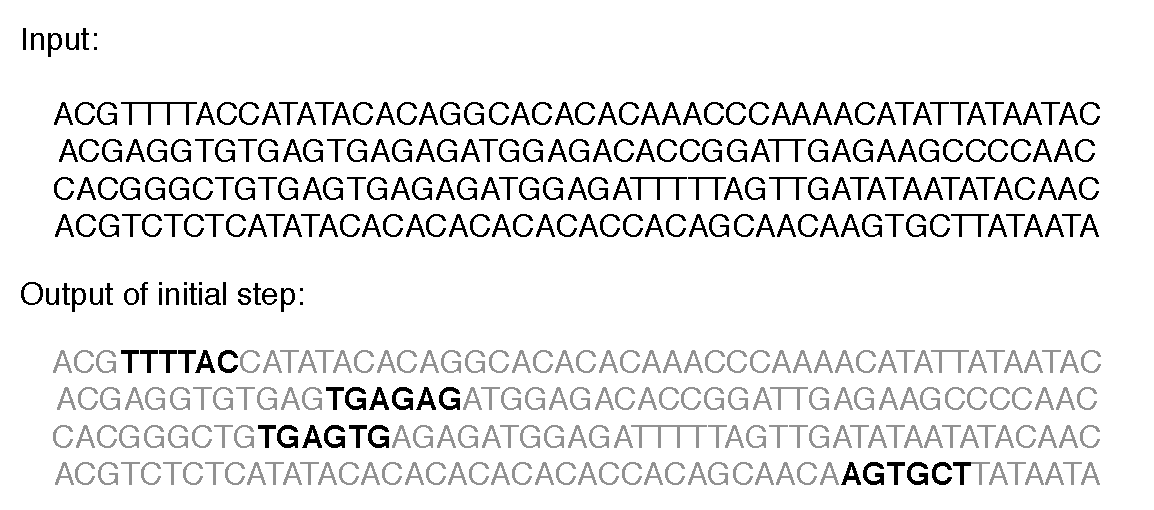
\includegraphics[width=\linewidth]{images/gibbs_example1}
\caption[An example showing the initialization step in Gibbs sampling.]{An example showing the initialization step in Gibbs sampling. The initial step of the Gibbs sampling algorithm chooses a subsequence of a given length from the input sequences uniformly at random.  The subsequences shown in bold are the selected subsequences from this step.}
\label{fig:gibbs_example1}
\end{center}
\end{figure}

At each iteration, the algorithm probabilistically decides whether to add a new site and/or remove an old site from the motif model, weighted by the binding probability for those sites. The resulting motif model is then updated, and the binding probabilities recalculated. Given sufficient iterations, the algorithm will efficiently sample the joint probability distribution of motif models and sites assigned to the motif, focusing in on the best-fitting combinations.  The algorithm repeatedly performs the following steps to iteratively improve the motif:
\begin{enumerate}
\item It selects a sequence $S_i$ at random from the set of input sequences and deletes its length-$\ell$ subsequence.
\begin{figure}[h!]
\begin{center}
 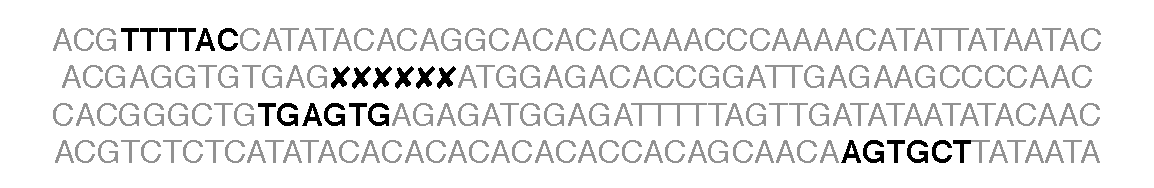
\includegraphics[width=\linewidth]{images/gibbs_example2}
\caption[Illustration of step 1 of Gibbs sampling. ]{Illustration of step 1 of Gibbs sampling.  In step 1 one of the subsequences is chosen randomly and the $\ell$-length subsequence is deleted.}
\label{fig:gibbs_example2}
\end{center}
\end{figure}
\item Next, it defines the PWM $\theta$ based on the remaining length-$\ell$ sequences ({\em i.e.} the subsequences in bold in Figure \ref{fig:gibbs_example2}), and the PWM $\theta_0$ based on the non-motif regions.
\item For each length-$\ell$ subsequence $s_{ij}$ from sequence $S_i$ and starting at position $j$, it calculates $\frac{\Pr(s_{ij} | \theta)}{\Pr(s_{ij} | \theta_0)}$, which is denoted as $score_j$.  
\item The algorithm then lets $\arg \max_{j} score_j$ be equal to $j$. 
\begin{figure}[h!]
\begin{center}
 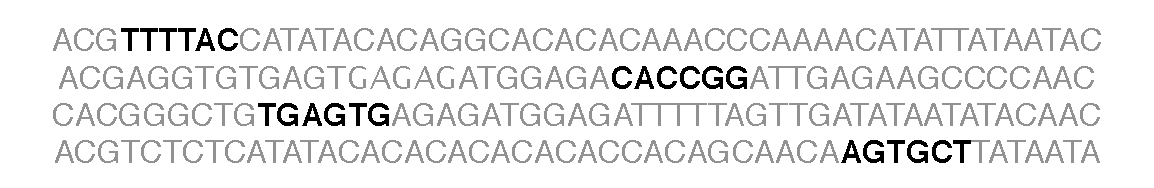
\includegraphics[width=\linewidth]{images/gibbs_example3}
\caption[Illustration of step 4 of Gibbs sampling. ]{Illustration of step 4 of Gibbs sampling.  After the score of each $\ell$-length in sequence $S_i$ is calculated the subsequence that has the maximum score is added, replacing the deleted subsequence in Step 1.}
\label{fig:gibbs_example3}
\end{center}
\end{figure}
\end{enumerate} 

It follows that at each iteration of the algorithm, one of the motif instances is replaced with an improved instance.  When using the Gibbs sampler, a different set of initially selected subsequences will result in a different final set and therefore, to obtain results that are close optimal, the algorithm has to be ran a number of times and the motif instance with the maximum score is returned.  There are several algorithms that use Gibbs sampling as a subroutine.  For example, AlignACE (Aligns Nucleic Acid Conserved Elements) \cite{RHEC} and BioProspector \cite{LBL} are motif-recognition programs that employ a Gibbs sampling strategy.   

\subsubsection{BioProspector}

BioProspector uses Gibbs sampling to search a list of sequences for potential regulatory motifs \cite{LBL}. Gibbs sampling first initializes the motif matrix using length-$\ell$ subsequences that are randomly selected from the input; then, it samples from all length-$\ell$ subsequences in the input sequences to update the PWM. The probability of selecting a length-$\ell$ subsequence is proportional to the likelihood of generating it from the current motif matrix over the likelihood of generating it from the non-motif background. The motif matrix is updated until convergence, or until a certain number of sampling iterations has been reached. BioProspector has several significant improvements compared to GibbsDNA. It uses a Markov model estimated from all promoter sequences in the genome to model adjacent nucleotide dependency and improve motif specificity. It also adopts two thresholds to allow each input sequence to contain zero or multiple copies of the motif \cite{LBL}.

\subsubsection{MDScan}

MDScan \cite{LBL02} is a motif-discovery program that combines two widely adopted motif search strategies: word enumeration \cite{bussemaker,ST03,vanHelden,vilo} and position-specific weight matrix updating \cite{BE95,HHS90,LBL}.  It has been shown to detect longer motifs with a greater number of degenerate positions, however, it is unable to detect $(15, 4)$-motifs with adequate accuracy \cite{LBL02}.
  
\subsubsection{CONSENSUS}

CONSENSUS is a greedy algorithm that is based on a matrix consensus of overrepresented motifs in a set of sequences, coupled with a phylogenetic assessment of the statistical robustness of this motif \cite{HS}.

\subsubsection{The YMF Approach}

The Yeast Motif Detection (YMF) approach calculates the $z$-score for each oligomer occurring in the data set and has been shown to successfully detect motifs in yeast genomes. The success of YMF in detecting transcription factor binding sites in the yeast genome is due to the simplicity of the problem: the short motif length and small number of degenerate positions. Unfortunately, YMF is not suitable for detecting motifs where the length is large and the number of degenerate positions is significant.

\subsection{Combinatorial Methods}

Combinatorial approaches to motif-recognition use the motif model given in Definition \ref{def:combinatorial_motif}. The aim of these methods is to solve progressively weaker and more computationally challenging problems with superior accuracy and efficiency. For example, WINNOWER, which was developed in 2000, was capable of solving of solving the $(15,4)$-motif problem with 20 sequences, each of which had length at most 700 bp \cite{PS00}, whereas PSM1, which was developed in 2005, was able to solve the $(18, 6)$-motif problem with 20 sequences, each of which has length at most 1000 bp, with increased accuracy. We will describe the following three combinatorial approaches to motif recognition in detail: SP-STAR, WINNOWER \cite{PS00}, and PROJECTION \cite{BT02}. 

\subsubsection{SP-STAR}
 
SP-STAR, developed by Pevzner and Sze \cite{PS00}, does an enumerative search but only over a restricted search space defined by the data instead of the entire space. First, a set of subsequences is chosen as the initial motif, and then the best possible motif is obtained by employing a local improvement heuristic that uses scoring function that evaluates the strength of the motif. Given a set of length-$\ell$ sequences $\{x_1, x_2, \ldots, x_n\}$, we define $SPscore$ as $\sum_{i, j} d(x_i, x_j)$.   We summarize SP-STAR in the following steps:
\begin{enumerate}
\item Let $X$ be the set of all length-$\ell$ subsequences in the $n$ input sequences $\{S_1, \ldots, S_n\}$.
\item For any length-$\ell$ sequence $x \in X$ chosen uniformly at random, do the following:
\begin{enumerate}
\item\label{step1} Find the set of $n$ length-$\ell$ sequences $\{s_1, \ldots, s_n\}$ such that $s_i$ is contained in $S_i$ for all $i$, and $d(x, s_i)$ is minimized. 
\item\label{step2} Let $x$ be a sequence that contains the alphabet symbol that occurs most frequently at each position and with ties broken arbitrarily. 
\item Repeat steps \ref{step1} and \ref{step2} until $SPscore$ of $\{s_1, \ldots, s_n\}$ cannot be further improved. 
\end{enumerate}
\end{enumerate}

The algorithm is rerun a number of times and the set of sequences that minimizes $SPscore$ is returned.  Further, the authors suggest that the local improvement steps ``may take a long time'' \cite{PS00} and therefore, should only be performed on a fraction of the best initial sets of sequences. Nonetheless, the number of sequences to be searched is approximately ${\ell \choose d} 3^d$. SP-STAR was successful in finding $(15,4)$-motif instances in data sets containing 20 sequences, each of which has maximum length 700 but failed to have reasonable accuracy when the sequence length exceeded 700 \cite{RBH05}. 

\subsubsection{WINNOWER}

WINNOWER is a simple graph-theoretic approach that represents a motif instance as a clique\footnote{A clique is a graph in which every pair of vertices is joined by an edge.}. WINNOWER first constructs a graph $G(V, E)$ by creating a vertex for every subsequence of length $\ell$ occurring in the input and adding an edge between all pairs of vertices corresponding to subsequences that are distance $2d$ apart and occurring in different input sequences. Now the problem of finding a $(\ell, d)$-motif corresponds to finding a clique of size $n$.  However, clique finding is NP-complete \cite{GJ} and therefore, WINNOWER proposes a method to detect and delete spurious edges to reveal sets of vertices whose corresponding subsequences are possible motif instances \cite{PS00}.    We note that $G$ is a $n$-partite graph\footnote{A $n$-partite graph is a graph where the vertices can be partitioned into $n$ disjoint sets and there are no edges between vertices in the same set.}. 

We define a vertex to be a {\em neighbour} of a clique $C$ if it is connected to every vertex in $C$, and a clique to be {\em extendable} if it has at least one neighbour in each of the $n$ partitions of $G$.  The algorithm is based on the observation that every edge in a maximal $n$-clique belongs to at least ${n-2}\choose{k - 2}$ extendable cliques of size $k$.  An edge is referred to as {\em spurious} if it does not belong to any extendable clique of size $k$.  WINNOWER then iteratively deletes spurious edges for increasing values of $k$ with the idea that only extendable cliques remain.

When $k = 1$, a vertex $u$ is a neighbour of a vertex $v$	if $(u, v) \in E$.  Every vertex that does not contain at least $n - 1$ neighbours is deleted (since it certainly cannot be in a clique of size $n$).  For $k = 2$, a vertex $u$ is a neighbour of an edge $v, w$ if $v$, $w$, and $u$ form a triangle.  Therefore, any edge that does not have $n - 2$  neighbours that are from different partitions is deleted from $G$.  For $k > 2$, WINNOWER relies on the observation that for any clique of size $n$, there are $n \choose k$ extendable cliques with $k$ vertices and thus, every edge on a $n$-clique must belong to at least ${n - 2}\choose{k - 2}$ extendable cliques of size $k$.  Any edge that is not contained in the required number of extendable cliques is deleted.  

\begin{figure}[h]
\begin{center}
 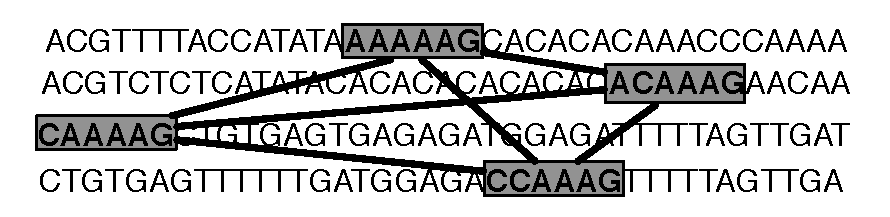
\includegraphics[width=\linewidth]{images/winnower}
\caption[An example showing a clique, which does not correspond to a motif set, in the graphical representation of the input used by WINNOWER. ]{An example showing a clique, which does not correspond to a motif set, in the graphical representation of the input used by WINNOWER. Let $\ell = 6$, $d = 2$, and $n = 4$.  In this example, we have set of sequences where each pair of sequences has distance at most $2d$ but there does not exist a length-$\ell$ sequence that has distance at most $d$ from each of the sequences in the set.}
\label{fig:winnower}
\end{center}
\end{figure}


One of the pitfalls of WINNOWER is that it does not actually report any motifs; it is only concerned with identifying cliques containing $n$ vertices.  Not all cliques correspond to valid motifs (according to the definition of Pevzner and Sze \cite{PS00}) and therefore, further analysis is required to distinguish cliques corresponding to valid motifs from those that are not.  See Figure \ref{fig:winnower} for an example of a set of sequences that corresponds to a clique but not a motif. 

The running time of the algorithm is $O(N^{2d + 1})$, where $N=nm$, and $m$ is length of the input sequences. The algorithm performs better than SP-STAR with the same data sets. However, due to the large number of spurious edges, the running time is prohibitively large and grows very rapidly as the motif strength weakens or subsequence length or number increases \cite{LSB04}.   

There have been many motif-recognition programs that have extended WINNOWER since its initial development.  In 2003, Liang {\em et al.}\ \cite{LSB04} presented cWINNOWER, which is essentially the WINNOWER algorithm with added constraints on the graph construction whose purpose is to reduce the number of spurious edges in the initial graph. Sze {\em et al.}\ \cite{SLC04} extended the graph formation of WINNOWER \cite{PS00}; they formulate the motif-finding problem as the problem of finding large cliques in $k$-partite graphs, with the additional requirement that there exists a string $s$ that is close to every motif instance.  Yang and Rajapakse \cite{YR04} adopted a graph formulation similar to Pevzner and Sze \cite{PS00}, then use a dynamic-programming approach to search for each clique of size $n$. The motif instances and center strings are then derived during the clique finding. Finally, a rescanning of the data set is done with the center string or the motif in order to find motif instances with Hamming distance less than or equal to $d$ from the center string. Lastly, PRUNER \cite{pruner} again uses the same graph formulation as Pevzner and Sze \cite{PS00} but deciphers between the cliques corresponding to a motif by further restricting the criteria for deleting an edge.  All of these algorithms -- cWINNOWER, the work of Sze {\em et al.}\ \cite{SLC04}, the work of Yang and Rajapakse \cite{YR04}, and PRUNER --  suffer from the limitation that an exorbitant amount of  time and space is needed to obtain decent results \cite{LSB04,pruner,SLC04,YR04}.

\subsubsection{Random Projection}

In 2002, Buhler and Tompa developed PROJECTION, an algorithm based on random projections \cite{BT02}.  Assume that we have an $(\ell, d)$-motif problem, and $s_m$ denotes the motif that we are interested in detecting.  PROJECTION considers all length-$\ell$ subsequences in the input set, and projects each of these subsequences along $k$ randomly chosen positions, where $k$ is some appropriately chosen value.  Hence, for every subsequence in $S$, generate a $k$-mer $u'$ that is a subsequence of $u$ corresponding to the $k$ random positions chosen.  Note that the random positions are the same for all the length-$\ell$ subsequences.  Hence, each length-$k$ subsequence is thought of as an integer.  We group the length-$k$ subsequences according to their integer values ({\em i.e.}\ all the length-$\ell$ subsequences are hashed using the length-$k$ subsequences of any length-$\ell$ subsequence as its hash value).  

If a hashed group has at least a threshold number $\alpha$ of length-$\ell$ subsequence in it then there is a good chance that $s_m$ will have its length-$k$ subsequence equal to the length-$k$ subsequence of this group.  Hence, choosing appropriate parameters is vital to the accuracy and efficiency of PROJECTION.  There are $n(m - \ell + 1)$ length-$\ell$ subsequences in the input and there are $4^k$ possible length-$k$ subsequences.  Therefore, the expected number of length-$\ell$ subsequences that hash into the same bucket is $n(m - \ell + 1)/4^k$. The threshold value $\alpha$ is chosen to be twice this expected value. The value of $k$ has to be chosen small enough so that a significant number of motif instances are grouped together under the projection but large enough so that non-motif instances are not grouped together with motif instances; {\em i.e.}\ $k$ is chosen such that $n(m - \ell + 1) < 4^k$ so that the expected number of random length-$\ell$ subsequences that hashed into the same bucket is less than one. 

The process of random hashing is repeated $r$ times to ensure that that a bucket size of at least $\alpha$ is observed at least more than once.  The value of $r$ is defined with respect to several other values which we now define. The probability $p$ that a given motif instance hashes to the planted bucket is equal to ${{{\ell - d}\choose{k}}}{{\ell}\choose{k}}$, and it follows that the probability that fewer than $\alpha$ hash into a bucket is $p' = \sum_{i = 1}^{\alpha - 1} {n\choose i} p^i (1 - p)^{\alpha - i}$.  Thus, the probability that fewer than $\alpha$ hash into a bucket in each of the $r$ trials is equal to $p'^{t}$, which we denote as $P$.  The value of $r$ is equal to $\lceil \frac{\log P}{ \log p'}\rceil$.  In the original paper of Buhler and Tompa, a value of $0.05$ is used for $P$ \cite{BT02}.  In the final step of the algorithm, the sets of length-$\ell$ subsequences that pass the threshold are collected and processed to obtain the motif sequences that are returned.

\subsubsection{The Voting Algorithm}

In 2005, Leung and Chin \cite{CL05} described two algorithms: the Voting algorithm and the Voting algorithm with projection.  The latter is capable of solving challenging motif problems ({\em i.e.}\ the $(9, 2)$, $(11, 3)$ and $(15,5)$ problems), as well as detecting motifs where $\ell$ and $d$ are ``large'' ({\em i.e.}\ the $(20, 7)$ and $(30, 11)$ problems). However, the Voting algorithm (by itself) cannot solve any motif problem when $\ell > 15$ due to heavy time and space requirements \cite{CL05}.  The Voting algorithm with projection uses a similar algorithm as a preprocessing step, then the Voting algorithm is used to recover the motif instances from the set of sequences hashed into the same bucket by projection.  

We give a brief description of the Voting algorithm.  We define a length-$\ell$ sequence $s'$ to be a {\em d-variant} of another length-$\ell$ sequence $s$ if the Hamming distance between $s'$ and $s$ is at most $d$.  We denote all the $d$-variants of a sequence $s$ as $N(s,d)$.  Note that if $s_m$ is a motif then $s_m$, along with all the instances are contained in $N(s_m, d)$.  Then for each length-$\ell$ subsequence $s_i$ in the input sequences gives a vote to each of the sequences in $N(s_i, d)$. Further, each length-$\ell$ sequence can get at most one vote from each of the $n$ input sequences, which ensures that a motif $s_m$ gets exactly $n$ votes. Although the basic Voting algorithm performs better than the basic enumeration algorithm, the required amount of space grows exponentially with $d$, rendering it impractical for reasonable sized values of $\ell$ and $d$.   

\subsubsection{Pattern Branching}

Pattern Branching is a local search algorithm that begins from subsequences that appear in the set of input sequences and systematically alters these initial sequences by changing one letter at a time in order to search for the center sequence \cite{patternbranching}.  If $s'$ is any length-$\ell$ sequence then there are ${{\ell}\choose{d}}3^d$ length-$\ell$ sequences that have Hamming distance $d$ from $s'$.  We refer to this set of sequences at the {\em neighbourhood} of $s'$.  One solution to the $(\ell, d)$-motif problem is to consider the neighbourhood of each of the $\ell$-mers in the set of input sequences, score each of the sequences appropriately, and then return the sequence with the highest score.  Since there could be at most ${{\ell}\choose{d}}3^d (n(m - \ell + 1))$ sequences, the space and time requirements of this basic algorithm are prohibitively large.  Nonetheless, there are several algorithms that use this approach \cite{GEW85,WAG84}.

Rather than considering all length-$\ell$ sequences in the neighbourhood of all occurring subsequences in $S$, Pattern Branching  only examines a selected subset of neighbours.  Again, we denote $N(s, d)$ to be all $d$-variants of $s$.  For any input sequence $S_j$ let $d_{min}(s, S_j)$ denote the minimum Hamming distance between $s$ and any length-$\ell$ subsequence of $S_j$.  Lastly, denote $d_{min}(s, S)$ to be $\sum_{j=1}^nd_{min}(s, S_j)$.  For any $\ell$-mer $s_{ij}$ in the input sequence $S_j$ let $BestNeighbour(s)$ be equal to the sequence in $N(s_{ij}, d)$ whose distance $d_min(s_{ij}, S)$ is minimum from all other sequences in $N(s_{ij}, d)$.  Pattern Branching starts from a sequence $s_{ij}$, identifies $s_{ij}^1 = BestNeighbour(s_{ij})$, then identifies $s_{ij}^{k + 1} = BestNeighbour(s_{ij}^{k})$ for all $1 \leq k \leq d - 1$. The best $s_{ij}^d$ among all possible length-$\ell$ subsequences of the input $S$ is output.

 
\subsubsection{Profile Branching}

Profile Branching \cite{PRP} is similar to Pattern Branching; the main difference between the two algorithms is that in the latter, the search space is of {\em motif profiles}, rather than motif sequences. Given an length-$\ell$ sequence $s = s(1), s(2), \ldots, s(n)$, we define the {\em profile} of $s$ to be a $4 \times \ell$ matrix $X(s)$ where each column is defined as follows:


\[x_{i \alpha} = \left\{ 
\begin{array}{l l}
	\frac{1}{2} 	& \quad \mbox{if $s(i) = \alpha$,}\\
  	\frac{1}{6}		& \quad \mbox{otherwise}\\ \end{array} \right. \]

For example, suppose $s = ACCA$ then the motif profile for $s$ is:

\begin{center}
\begin{tabular}{ l | l l l l }
  ~ & 1 & 2 & 3 & 4 \\
  \hline
  A & $\frac{1}{2}$ & $\frac{1}{6}$ & $\frac{1}{6}$ & $\frac{1}{2}$ \\
  C & $\frac{1}{6}$ & $\frac{1}{2}$ & $\frac{1}{2}$ & $\frac{1}{6}$ \\
  G & $\frac{1}{6}$ & $\frac{1}{6}$ & $\frac{1}{6}$ & $\frac{1}{6}$ \\
  T & $\frac{1}{6}$ & $\frac{1}{6}$ & $\frac{1}{6}$ & $\frac{1}{6}$ \\  
\end{tabular}
\end{center}

The algorithm proceeds identically to Pattern Branching but now the sequences in are ranked according to a new score function, which is referred to as the {\em entropy score}.  The Pattern Branching algorithm outperforms the Profile Branching algorithm; however, the latter does not obtain acceptable accuracy when the degeneracy $d$ is large relative to the sequence length $\ell$ \cite{PRP}.   

\subsection{Challenge Problems} \label{challenge_problems_section}

Pevzner and Sze defined the weak motif-recognition problem more concretely by illustrating the limitations of most motif-recognition programs; their results illustrate that although most methods at the time were capable of finding motifs of length 6 with no degeneration, most failed to detect motif instances of length 15 with 4 degenerate positions in a random sample containing 20 sequences, each of which has length 600 bp \cite{PS00}.  Since this problem was defined, many approaches have been developed with the intention of detecting motifs that have a relatively large number of degenerate positions.  Pevzner and Sze coined the phrase ``challenge problems'' to denote problems where the motif degeneracy ({\em i.e.} parameter $d$) is relatively large with respect to the motif length ({\em i.e.} the parameter $\ell$). Since then the phrase has been commonly used and pertains to problems such as the $(12, 3)$, $(15, 4)$, and $(18, 6)$ motif problems as well as many others. 

\subsection{Exact Verses Approximate Algorithms} \label{approximate_solution_section}

Algorithms that are exact are referred to as {\em exhaustive enumeration algorithms} in the literature.  Many exact motif-recognition algorithms are known ({\em e.g.}\ \cite{BJVU98,GEW85,m83,RBH05,ST00,staden,tompa99,vHAC-V}, however, the running times of these algorithms are prohibitively large for any of the challenge problems \cite{BT02}. Exact algorithms are guaranteed to determine the motif and motif instances, whereas, the solution determined by an approximate algorithm is likely to mismatch with the correct motif and motif instances at a number of positions.  We define the {\em success rate} of a given program using the performance coefficient used by Pevzner and Sze \cite{PS00}, Buhler and Tompa \cite{BT02}, and others \cite{CL05,CL06}. 

\begin{definition} ({\bf performance coefficient}) Let $K$ denote the set of $t\ell$ base positions in the $t$ occurrences of the planted motif, and let $P$ denote the corresponding set of base positions in the $t$ occurrences predicted by an algorithm.  The algorithm's success rate is defined as $|K \cap P| / |K \cup P|$.\end{definition}

\noindent A performance coefficient of $0.75$ or greater is acceptable for algorithms not guaranteeing exact accuracy. The success rate of a program will arise when evaluating motif recognition programs. 

Approximate algorithms, such as CONSENSUS \cite{HS}, Gibbs \cite{LABLNW}, MEME \cite{BE95}, and ProfileBranching \cite{PRP} take significantly less time but perform poorly on finding weak motifs; for example (15,4)-motifs are almost completely undetectable using these programs \cite{HHS90}. More recently, there have been a number of programs that are approximate but have decent performance coefficients (over 75\%), including PROJECTION \cite{BT02}, the Voting algorithm \cite{CL05}, PSM1 \cite{RBH05} and PMSprune \cite{JBR07}.  Unfortunately, most programs failed to achieve decent performance coefficients in practical running time for all $(\ell, d)$-motifs we tested.  The details of these experiments will be discussed in depth in later chapters. 

\section{Past Work on the String Selection Problems}

The {\sc Closest String} problem has not only generated a significant amount of research interest in itself, but is also an important subproblem of motif recognition. We will discuss some past results concerning this problem, and later in this thesis, we develop and apply some efficient heuristics for this problem.  

\subsection{The {\sc Closest String} Problem}

Stojanovic {\em et al.}\ \cite{sto} provided a linear-time algorithm for the case $d=1$. There exists a trivial fixed parameter tractability algorithm when $\ell$ remains fixed: simply try all possible $|\Sigma^{\ell}|$ strings.  Gramm {\em et al.}\ \cite{GNR03}  demonstrated that the {\sc Closest String} problem is in FPT when the number of strings $n$ remains fixed.  This parameterized tractability result is based on an integer linear programming formulation with a constant number of variables, and the application of the result of Lenstra \cite{Len}, which states that integer linear programming is polynomial-time solvable when the number of variables remains fixed. Unfortunately, such an integer linear programming formulation is only of theoretical interest since the corresponding algorithms lead to very large running times even when the number of strings is small. When $d$ is fixed, the problem can be solved in $O(nl + nd(d + 1)^d)$ time \cite{GNR03}.  Ma and Sun gave an $O(n |\Sigma|^{O(d)})$ algorithm, which is a polynomial-time algorithm when $d = O(\log n)$ and $\Sigma$ has constant size \cite{MS08}. Most-recently, Wang and Zhu designed an $O(\ell n + nd|\Sigma|^d 2^{3.25d} )$ time fixed parameter algorithm for the {\sc Closest String} problem \cite{WZ}. Chen {\em et al.}\ \cite{CMW} and Zhao and Zhang \cite{ZZ} also improved upon the fixed parameter tractable result of Ma and Sun \cite{MS08}. 

Ben-Dor {\em et al.}\ \cite{BLPR} used a standard linear programming and randomized rounding technique to develop a near-optimal algorithm for large $d$ ({\em i.e.}\ when $d$ is super-logarithmic in the number of strings).  Lanctot {\em et al.}\ \cite{LLMWZ00_v1} gave an approximation algorithm for the {\sc Closest String} problem that achieves a worst case performance ratio of 2.  It is a simple algorithm that constructs an approximate feasible solution in a pure random fashion.  Starting from an empty solution, the algorithm selects at random the next element to be added to the solution under construction.  In subsequent work, Lanctot {\em et al.}\ \cite{LLMWZ00} gave a polynomial-time algorithm that achieves a $\frac{4}{3} + o(1)$ approximation guarantee. Independently, G\c{a}sieniec {\em et al.}\ \cite{GJL} gave a $\frac{4}{3}$-approximation algorithm that uses a similar technique. This improved algorithm is based on a linear programming relaxation of an integer programming model of the {\sc Closest String} problem.   The basic idea consists of solving the linear programming relaxation\footnote{The linear programming relaxation of an integer program is the problem that arises by replacing the constraint that each variable must be an integer in the set $\{0, 1, \ldots, k\}$ by a weaker constraint, that each variable belong to the interval $[0,k]$.} and using the result of the relaxed problem to define an approximate solution to the original problem.   More specifically, Lanctot {\em et al.}\ \cite{LLMWZ00} used randomized rounding for obtaining an integer 0-1 solution from the continuous solution of the relaxed problem; this technique works by letting a Boolean variable $x$ in the linear program be equal to one with probability $y$, where $y$ is the value of the continuous variable corresponding to $x$ in the relaxation of the original integer program.  

Using randomized rounding again, Li {\em et al.}\ \cite{LMW02} proved the existence of a PTAS for this problem.  Unfortunately, the high degree in the polynomial complexity of the PTAS algorithm renders this result only of theoretical interest.  For a given value of $r$, all choices of $r$ subsequences of length $l$ are considered from the $n$ sequences. The algorithm runs in $O(l(nm)^{r + 1})$-time, which is polynomial for any constant $r$.  In 2005, Brejov\'{a} {\em et al.} \cite{brona1} proved the existence of sharper upper and lower bounds for the PTAS on a slight variant of the {\sc Closest String} problem (which they refer to as the {\sc Consensus Pattern} problem) and in 2006, Brejov\'{a} {\em et al.} \cite{brona2} improved upon the analysis of the PTAS for various random binary motif models by showing that there are known ``weak'' instances for which the approximation ratio is $1 + \Theta(1/ \sqrt{r})$ \cite{brona1}, and ``strong'' instances for which the PTAS will be guaranteed to determine the correct answer in efficient time.  Andoni {\em et al.}\ \cite{AIP} gave a novel PTAS that has improved time complexity, and most recently, Ma and Sun \cite{MS08} presented a PTAS with time complexity $O(n^{\Theta(n^{-2})})$, which is currently the best known. 

\subsection{The {\sc Farthest String} Problem}

Lanctot {\em et al.}\ proved the existence of a PTAS for this problem, though the high degree in the polynomial complexity of the PTAS algorithm renders this result only of theoretical interest \cite{LLMWZ00}.  The algorithm is based on the randomized rounding of the relaxed solution of an integer programming formulation.  There have been no improvements on the running time of this PTAS. 

In 2004, Cheng {\em et al.}\ \cite{cheng} gave a $O((|\Sigma|(\ell-d_f)) (\ell-d_f))$ fixed parameter algorithm for the {\sc Farthest String} problem. This fixed parameter tractability algorithm is nearly identical to the algorithm of Gramm {\em et al.}\ \cite{GNR03} for the {\sc Closest String} problem. Most recently, Wang and Zhu gave a $O(\ell n+n d 2^{3.25d_f})$ fixed parameter algorithm for the {\sc Farthest String} problem when the input strings are binary strings \cite{WZ}. 

\section{Summary}

In this chapter, we surveyed some of the important results in motif recognition, the {\sc Closest String} problem, and its variants.  We described two motif-recognition models, including the combinatorial model that was formally introduced by Pevzner and Sze \cite{PS00}.  Since the combinatorial version of this problem was initially described, there has been a plethora of research in developing motif-recognition programs that are efficient and capable of solving computational challenging instances of this problem.  We continue this area of research by developing  an efficient motif-recognition program that is based on a novel weighted graph model, and illustrating how combinatorial and probabilistic insights can be applied to gain even more efficiency and capability in solving computationally challenging instances of motif recognition. 
%======================================================================
\chapter{MCL-WMR: a Comprehensive Motif-Recognition Algorithm}\label{chapter:mclwmr}
%======================================================================

In Chapter \ref{chapter:related_work} we described the motif-recognition problem in detail, and described several other motif-recognition programs.  Pevzner and Sze defined the weak motif-recognition problem more concretely by illustrating the limitations of most motif-recognition programs; their results illustrate that although most methods at the time were capable of finding motifs of length 6 with no degeneration, most failed to detect motif instances of length 15 with 4 degenerate positions in a random sample containing 20 sequences that were 600 nucleotides long \cite{PS00}.  Since these challenge problems were defined, many approaches were developed with the intention of detecting motifs that have a relatively large number of degenerate positions.  In this chapter we describe a new approach for this problem, and provide theoretical and experimental results that support our approach.

Our algorithm, MCL-WMR, builds a weighted graph model of the input data and uses a graph clustering algorithm to quickly determine important subgraphs that need to be searched further for valid motifs. We compare the results of MCL-WMR to that of previously developed approaches; testing on synthetic data has shown that MCL-WMR has competitive running time capabilities and accuracy.  An added advantage of MCL-WMR is the ability to detect multiple motif instances. 

As previous described, the {\sc Closest String} problem asks, given a parameter $d$ and a set $S = \{s_1, \ldots, s_n\}$ of $n$ strings, each of length $\ell$, whether there exists a string that has Hamming distance at most $d$ from each of the strings in $S$. The following definition will be useful in this and later chapters:

\begin{definition} {\bf (weight of a set of sequences)}\label{def:weight} Given a set $S = \{s_1, s_2, \ldots, s_n\}$ of $n$ sequences, each of length $\ell$, we define the {\em weight} of the set $S$ to be $\sum_{i = 1}^n \sum_{j = i}^n  \ell - d(s_i, s_j)$.  \end{definition}

For a given parameter $d$ we say $S$ is a {\em motif set} if there exists a center string $s^*$ at distance at most $d$ from any string in $S$; we say a set $S$ of strings is {\em pairwise bounded} if the distance between any pair of strings in $S$ is at most $2d$.  Every motif set is pairwise bounded; if a pairwise bounded set is not a motif set we say it is a {\em decoy set}.  For example, for $d=1$ the set $\{000, 001, 010, 100\}$ is a motif set because $000$ is a center string for this set.  In contrast, the set $\{000, 011, 101, 110 \}$ is a decoy set because it is pairwise bounded (since any two of the strings are at Hamming distance at most two) but no center string exists.  We introduce the exploration of using the weight of a set as an indicator of whether a {\sc Closest String} instance is a motif set or a decoy set. 

\section{System and Methods} \label{section:mcl_wmr_system}

MCL-WMR involves three stages: graph construction, clique finding using graph clustering, and recovering the motif instances and their center strings. An overview of MCL-WMR is shown as follows: 

\begin{algorithm*}
\caption{An overview of MCL-WMR}
\begin{algorithmic}
\STATE  \% build the graph from the given data
\STATE{\bf for }each of the subgraphs{ \bf do}
 \STATE \hspace{5mm}cluster subgraph using MCL
 	\STATE\hspace{5mm}{\bf for} each cluster {\bf do}
	\STATE\hspace{10mm}{\bf if} the weight of the current cluster is above $threshold$ {\bf then}
	\STATE\hspace{15mm}search that cluster to see if it contains a motif	
	\STATE\hspace{15mm}if we find a motif, we are done.
\end{algorithmic}
\end{algorithm*}

\noindent The MCL-WMR algorithm first chooses a {\em reference sequence} from the data set, denoted as $S_r$, building the entire graph from all the input data (including $S_r$), and for each vertex $v_{r \Sigma}$ representing the length-$\ell$ subsequence from $S_r$ starting at position $\Sigma$.  We then use the Markov Cluster Algorithm (MCL) \cite{vD00} to generate subgraphs which contain vertices that are highly inter-related. From these clusters of vertices we will generate the positions of the possible motif instances and their corresponding center string. The algorithm terminates when a motif is found.  In order to increase the probability that a motif is found, we minimize searching subgraphs with low probability of containing a motif; hence, the adjacency subgraphs are not clustered and searched in a sequential manner.
  
\subsection{Graph Construction}\label{graph_construction} 

In our graphical representation of the data set, each subsequence of length $\ell$ is represented by a vertex and the construction of our graph ensures that the motif instances represented by vertices in the graph are connected to each other and form a clique of size $n$ (though the converse need not hold).  Thus, the weak motif-recognition problem is converted to finding cliques with size $n$ in our constructed graph $G$ which is defined as follows:

\begin{enumerate}
\item The vertex set contains a vertex $v_{i,j}$ representing the $\ell$-length subsequence in sequence $i$ starting at position $j$, for each $i$ and $j = 1, 2, \dots, m-\ell+1$. There are $n(m-\ell+1)$ vertices.
\item Each pair of vertices $v_{i,j}$ and $v_{i',j'}$, for $i \neq i'$ is joined by an edge when the Hamming distance between the two represented subsequences is at most $2d$.
\item An edge between vertices having distance $k$ has weight $\ell - k$ for $d < k \leq 2d$, or $10(\ell-k)$ for $k \leq d$.  This emphasizes subsequences at small distances.
\end{enumerate}

\noindent This graph is represented by a symmetric adjacency matrix, where each entry is 0 for a non-edge, or a positive weight for an edge. This representation takes $O((n(m-\ell+1)^2))$ space and is constructed in $O(n^2(m-\ell)(m+\ell))$ time. Since the graph is $n$-partite, a clique of size $n$ contains exactly one vertex from each sequence. 

We reduce the size of the instance being passed to MCL by considering subgraphs $\{G_0, G_1, \dots, G_{m-1}\}$, where $G_i$ is the subgraph induced by the vertex corresponding to the reference sequence (denoted as $v_{R,i}$), and its neighbours (for some arbitrary choice of reference sequence $R$) instead of searching all of $G$ at once. Therefore, we have reduced the problem of finding weak motifs in the input data set $S$ to finding cliques of size $n$ in the $G_i$, though, some cliques may not correspond to valid motifs. Figure \ref{fig:graph_construction} illustrates this weighted graph construction of the input sequences.  

\begin{figure}[!h]
\begin{center}
 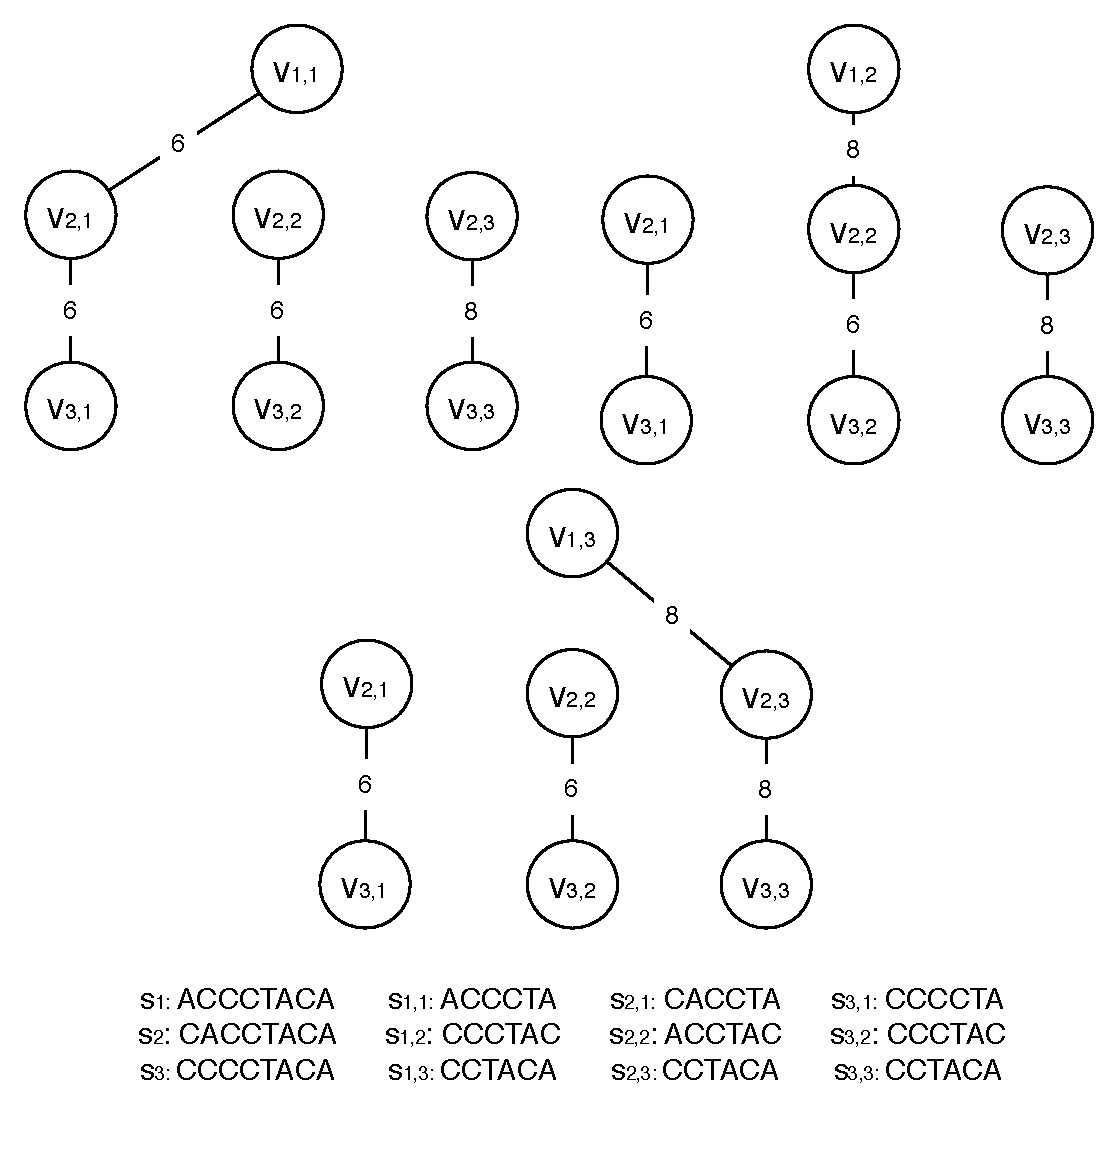
\includegraphics[width=\linewidth]{images/graph_construction}
\caption[An example showing the weighted graph representation of the input data used by MCL-WMR.]{An example showing the weighted graph representation of the input data used by MCL-WMR. The three input sequences are shown at the bottom-left corner of the figure. We have $n=3$, $m=8$, $\ell=6$, $d=1$. }
\label{fig:graph_construction}
\end{center}
\end{figure}

\subsection{Using Clustering to Find Motifs}

A {\em clustering} of graph is a decomposition of the vertex set into subsets of vertices that are highly intra-connected and, hence, induce dense subgraphs. A {\em good clustering} of a graph  is an approximation of a partitioning of the graph into cliques. A clique corresponding to a motif will exist in one of the subgraphs of $G$ since each motif instance appears as a vertex in a clique of size $n$.  We use MCL \cite{vD00} to cluster the sets of vertices to determine subgraphs that are highly intra-connected with high-weight edges, and sparsely inter-connected and thus likely to correspond to a motif instance.  We chose MCL because it is able to handle weighted graphs, and because it efficiently handles large undirected graphs. The idea underlying the MCL algorithm is that dense subgraphs correspond to regions where the number of length $k$ paths is relatively large, for small $k$. Random walks of length $k$ have higher probability for paths beginning and ending in the same dense region than for other paths.   

The MCL process consists of the alternation of two operations, namely {\em expansion} and {\em inflation}.  The image of a stochastic matrix under expansion is just some finite power of the matrix.  The image of a (column) stochastic matrix under inflation is formed by raising each entry of the matrix to the same positive power, followed by a rescaling of the columns such that the result is stochastic again.  An MCL process is defined by a column stochastic input matrix $T_1$ and two rows of exponents $e_{(i)}$, $r_{(i)}$, resulting in a row of stochastic matrices $M_{(i)}$, defined by:$$T_{2i} = \exp_{e_i} (T_{2i - 1}),  \,\,	i = 1, \ldots, n$$ $$T_{2i + 1} = \Sigma_{r_i} (T_{2i}),	\, i = 1, \ldots, n$$ where $\exp_{e_i}(T)$ is $T^{e_i}$ and $e_i \in \mathcal{N}$ and $r_i \in \Re$, $r >0$.  The image under the {\em inflation operator} $\Sigma_r$ of a nonnegative matrix $M \in \Re^{k \times \ell}$ having no zero columns is defined as: \[(\Sigma_rM)_{pq} = (M_{pq})^r \/ \sum^{k}_{i = 1} (M_{iq})^r. \] The largest transition probabilities will generally correspond with nodes lying in the same natural cluster; this effect is boosted in the MCL process via the inflation operator. By expansion, transition probabilities corresponding with random walks of higher length are computed.  The inflation operator promotes larger transition probabilities at the cost of small probabilities and thus, promotes random walks between nodes lying in the same cluster and demotes random walks between nodes lying in different clusters. 

\subsection{Recovering Motifs}

MCL produces sets of vertices that produce dense regions of the subgraph $G_i$; we filter the subgraphs obtained from MCL to subgraphs that have high probability of containing a motif.  A clique in $G$ that represents a motif instance must have size $n$ and have weight greater than or equal to $( \ell - 2d) {n \choose 2}$ since each pair of vertices are adjacent.  We filter out clusters that do not meet these criteria. Clusters that pass this test may contain multiple cliques formed by choosing different subsets of $n$ cluster vertices, or possibly no cliques at all. We identify all ways of forming a clique from the cluster vertices by using the $n$-partite nature of the graph to explore all possible cliques with the following depth-first search algorithm.  The dynamic-programming algorithm we use is as follows:

\begin{enumerate}
\item Let the sets $\mathcal{C} = {\mathcal{C}_r , \mathcal{C}_2, \ldots, \mathcal{C}_n}$ represent the subsets of vertices in a cluster that need to be considered.  Hence,  $\mathcal{C}_r = \{v_{r\sigma}\}$, $\mathcal{C}_2 = \{v_{21'} , v_{22'}, \ldots, v_{2|\mathcal{C}_2|'} \}$, $\ldots$, $\mathcal{C}_n = \{v_{n1'} , v_{n2'}, \ldots, v_{n|\mathcal{C}_n|'} \}$. Note that $\mathcal{C}_r$ contains only one vertex since it is the reference sequence. 
\item Lists $\mathcal{L}_{ij'}$, for $i = r$ and $j' = \sigma$ and $i = 2, \ldots, n$ and $j' = 1, \ldots, |\mathcal{C}_i|$ are created as follows: 
\begin{enumerate}
\item Set $\mathcal{L}_{r\sigma} = \emptyset$. 
\item Set $\mathcal{L}_{2j'} = \{v_{r\sigma} \}$ for vertex $v_{2j'} \in \mathcal{C}_2$. 
\item for $i = 3, \ldots, n$ 
\begin{description}
\item[~] Set $L_{ij'} = \emptyset$ for $v_{ij'} \in \mathcal{S}_i$
\item[~] for each vertex $v_{i -1k'} \in \mathcal{C}_{i−1}$, $k' = 1, \ldots, |\mathcal{C}_{i−1}|$
\begin{itemize}
\item if $d(v_{ij'}, v_{i-1k'} ) \leq 2d$ then let $\mathcal{L}_{ij'}$ be equal to $\mathcal{L}_{ij'} \cup \{ v_{i-1k′} \} \cup \mathcal{L}_{i-1k'}$
\end{itemize} 
\end{description}
\end{enumerate}
\item If a clique with size $n$ exists then there must exist a list $\mathcal{L}_{nj'}$ for vertices $v_{nj'} \in \mathcal{C}_n$ that contains vertices from each set $\mathcal{C}_i$ for $i = 1, \ldots, n -1$. 
\end{enumerate}

For each such clique found using the above dynamic-programming algorithm, we test if it represents a motif instance by attempting to find a string that has distance at most $d$ to every vertex. We do this by building up a list of possible center strings and the number of mismatches to each vertex for each possibility, one character at a time. Once a candidate string has $d+1$ mismatches to some vertex, it is discarded. Although the space of $4^{\ell}$ possible center strings is very large, in practice the list is pruned very rapidly on the $d+1$st character, {\em i.e.}\ after reaching size $4^d$.

We use a heuristic to determine a center string which tries all possible length $\ell$ DNA sequences that have high probability of having distance at most $d$ from each string in the set $S$ and thus, determines whether the subsequences are $(\ell, d)$-motifs.  In practice this dynamic-programming algorithm is quite efficient because the size of the clusters returned by MCL is small.  After obtaining the possible motif instances from $s_n$, the corresponding likely center string is found by alignment of the $n$ sequences and lastly, in order to determine if the set of subsequences found are motif instances it is checked that each subsequence is of distance at most $d$ from the center string.  As the sequences become longer or $d$ becomes large relative to $\ell$, the number of spurious cliques found will increase; this final step guarantees that the found subsequences are proper motif instances. 

\section{Analysis of Graph-Theoretic Model}

To validate our approach of using edge weights to assist in the search of valid motifs we show the existence of a separation between the weight of a set of sequences corresponding to a motif set and that of a set of sequences that does not correspond to a motif set.  We prove that the weight of an arbitrary set of subsequences corresponding to a motif set deviates from the mean with low probability.  Empirical results support the analytical description of the distribution and show that for a  typical motif-recognition problem ({\em i.e.} when $\ell = 15$ and $d = 4$) there exists a separation between the distribution of the weights of the motif sets and those of the decoy sets.

\subsection{Analysis of the Weight of a Clique Containing a Motif} \label{section:mcl_wmr_analysis}
 

Consider a clique $C$ that contains a set of subsequences corresponding to a motif set. Let $W$ be the random variable for the sum of each of the ${n \choose 2}$ edge weights in $C$. Let $v_1, v_2, \ldots v_n$ be the set of $n$ vertices in $C$ corresponding to sequences $s_1, \ldots, s_n$.  We seek the mean of $W$ and a tail bound for large deviations from the mean.  Let $W_i$ be the expected value of the random variable $W$ given that the first $i$ subsequences in $C$ are known.  

We prove several results concerning random $(\ell, d)$-motif sets.  A standard method used to generate a random $(\ell, d)$-motif set is to choose an $\ell$-length sequence uniformly at random from all possible $|\Sigma|^{\ell}$ sequences to be the center string, and then form a motif set by selecting $n$ sequences at random with replacement from the set of all sequences with Hamming distance at most $d$ from this center string \cite{BT02}.  This samples motif sets with probability proportional to the number of distinct center strings it has and thus, corresponds to how synthetic problem data sets are constructed and how we expect meaningful motif sets arise in nature.  For example, synthetic problem instances are traditionally generated as follows: a random center string of length $\ell$ is chosen, $n$ occurrences of the motif are generated by randomly mutating at most $d$ positions, and each of the $n$ motif instances is embedded at a random location into a different background string of length $m$.  We note that other non-uniform distributions have also been used to generate motif sets \cite{PS00}. 

\begin{theorem}  \label{mean_thm} The expected weight of a clique in $G$, which models a random $(l,d)$-motif problem containing $n$ sequences, is  \[ E[W] = {n \choose 2} \left( \ell -  \frac{1}{\beta^2}  \sum_{a=0}^{d} \sum_{b=0}^{d}{{\ell} \choose b}{{\ell} \choose a}3^{a + b} \left(  a+b-\frac{4ba}{3l}\right) \right) \] where $\beta= \sum_{i = 0}^{d} {{\ell} \choose i} 3^i$. \end{theorem}

\begin{proof} Given an $(\ell, d)$ motif set $S$, we aim to compute the expected value of the weight of the set $S$ ({\em i.e.} $E[\sum_{i=1}^{n}\sum_{j=i+1}^{n}(\ell - d(s_i,s_j))]$.  Let $\mu_e$ be $E[d(s_i,s_j)]$ for any pair of sequences $s_i$ and $s_j$, where the corresponding vertices $v_i$ $v_j$ are joined by an edge in the clique that contains $S$.

\[ E \left[ W \right] =  E \left[ \sum_{\forall v_i, v_j, i < j} (\ell - d(s_i, s_j)) \right] = {n \choose 2} \mu_e \]
 
We choose the $n$ sequences uniformly from the $\beta = \sum_{i = 0}^{d} {{\ell} \choose i} 3^i$ possible choices. Let $s$ be a center string for the $\alpha_i$ denote the Hamming distance between $s_i$ and the center string $s$.  The expected weight of an edge will depend on the distance of the two sequences from the center string, so we break the expectation into pieces, as follows:

\begin{center}
\begin{math}	
\begin{array}{lll}
\mu_e  	& = & \sum_{\alpha_i = 0}^{d}\Pr[d(s, s_i) = \alpha_i ] E[d(s_i,s_j)| d(s, s_i) =\alpha_i ] \\
					& = & \sum_{\alpha_i = 0}^{d}\Pr[d(s, s_i) = \alpha_i ] \cdot  \sum_{\alpha_j=0}^{d}\Pr[d(s, s_j) = \alpha_j ]  \\
                    & ~  &  E[d(s_i,s_j)|d (s, s_i ) = \alpha_i, d (s, s_j ) = \alpha_j ] \\
					& = & \sum_{\alpha_i = 0}^{d}\frac{ {{\ell} \choose {\alpha_i}}3^{\alpha_i}}{\beta}\sum_{\alpha_j=0}^{d}\frac{{{\ell} \choose {\alpha_j}}3^{\alpha_j}}{\beta}E[d(s_i,s_j)|d (s, s_i ) = \alpha_i, d(s, s_j ) = \alpha_j ] \\
\end{array}
\end{math}
\end{center}	

The remaining problem is to compute the expected Hamming distance between $s_i$ and $s_j$, knowing that the sequences consist of copies of $S$ with $a$ and $b$ positions mutated, respectively. If a position was mutated in neither string it is a match; if a position was mutated in one sequence but not the other it is a mismatch; if a position was mutated in both sequences, it is a match with probability $\frac{1}{3}$.

If $s_i$ is fixed, $s_j$ consists of $b$ mutations that each either hit one of the $a$ mutated positions in $s_i$ or one of the other $\ell - a$ positions, sampled without replacement. The number that hit the $a$ mutated positions in $s_i$ follows a hypergeometric distribution with mean $\frac{ba}{\ell}$. If the number of hits to mutated positions is $c$, the expected total number of mismatches is: $b-c$ positions that hit among the $\ell-a$ non-mutated positions in $s_i$, $a-c$ positions among the $a$ mutated positions of $s_i$ that were \emph{not} hit, and $\frac{2}{3}c$ mismatches from the hits among the mutated positions, for a total of $(b-c)+(a-c)+\frac{2}{3}c = a+b-\frac{4}{3}c$. Therefore, $E(d(s_i,s_j)|d(s,s_i)=a, d(s,s_j)=b) = a+b-\frac{4ba}{3\ell}$. 

Therefore, $\mu_{e}$ is equal to $\ell -  \frac{1}{\beta^2}  \sum_{a=0}^{d}{{\ell} \choose a}3^a\sum_{b=0}^{d}{{\ell} \choose b}3^b \left(  a+b-\frac{4ba}{3\ell} \right) $, the expected weight of a single edge. 

\begin{center}
\begin{math}	
\begin{array}{lll}
E \left[ W \right] 	&=& {n \choose 2} \left( \ell -  \frac{1}{\beta^2}  \sum_{\alpha_i=0}^{d}{{\ell} \choose {\alpha_i}}3^{\alpha_i}\sum_{\alpha_j =0}^{d}{{\ell} \choose \alpha_j}3^{\alpha_j} \left(  \alpha_i+ \alpha_j-\frac{4\alpha_i \alpha_j }{3\ell} \right) \right) \\		
 							&=& {n \choose 2} \left(\ell -  \frac{1}{\beta^2}  \sum_{\alpha_i =0}^{d} \sum_{\alpha_j =0}^{d}{{\ell} \choose {\alpha_j}}{{\ell} \choose {\alpha_i}}3^{\alpha_i + \alpha_j} \left(  \alpha_i +\alpha_j - \frac{4\alpha_i \alpha_j }{3l}\right) \right) \\		

\end{array}
\end{math}
\end{center} \hfill $\Box$	\end{proof}

We are able to bound the probability of $W$ deviating from its mean by first demonstrating that $W_0, W_1, \ldots,$ $W_n$ is a martingale sequence and next, applying Azuma's inequality \cite{MR95} to determine the probability of a specific deviation.

\begin{theorem}  \label{azuma_thm} Consider the $(\ell,d)$-motif problem containing $n$ sequences. Let $W$ be the sum of the ${n \choose 2}$ edge weights in an arbitrary clique in $G_{motif}$ that corresponds to a motif set and let $\mu_W$ be the expected weight of the motif set, then for any $\lambda > 0$,  
\[\Pr[|W - \mu_W| \geq \lambda] \leq 2 \exp \left( - \frac{\lambda^2}{2d^2(n + 1)}  \right) \]
\end{theorem}

\begin{proof} Recall that $W_i$ is the expected value of the random variable $W$ given that the first $i$ sequences in $C$ are known and hence, the distances between the center string $s$ and the first $i$ vertices are known. Without loss of generality we choose a center string $s$ and let $\mathrm{F}_i$ be the $\sigma$-field generated by the random choice of the sequence $s_i$ from the set of all sequences at most distance $d$ from $s$.  It follows that, $W_i = [W | \mathrm{F}_i]$ since $W_i$ denotes the conditional expectation of $W$ knowing the first $i$ subsequences and therefore, $W_0, W_1, \ldots, W_n$ is a martingale sequence \cite{MR95}, with $W_0 = E[W]$ and $W_n = W$.

We now focus on the value $W_i - W_{i - 1}$.  Let $\Delta_{i, e}$ be the change in the random variable representing the weight of an edge $e$ from knowing the first $i -1$ sequences to knowing the first $i$ sequences. The value of $\Delta_{e, i}$ is non-zero for edges where the sequence corresponding to one of the endpoints of that edge was previously not known and is now known.  Each vertex in the clique is adjacent to $n - 1$ vertices; $i - 1$ of these vertices have corresponding sequences that were known and $n - i$ of these vertices have corresponding sequences that were unknown; all other ${n \choose 2} - n + 1$ remaining edges in the clique have no change in the expected value. In both cases, the expectation of the weight of the edge can change by at most $d$. Again, $\mu_{e}$ is the expected value when neither sequences $s_i$ or $s_j$ corresponding to the endpoints of the edge $e = (s_i, s_j)$ are known and therefore, we have the following: 

\[ |W_{i} - W_{i - 1}| \leq \Delta_{i, e} (n - 1)  = d (n - 1) \]
 

\noindent We have shown that the random variables $W_0, W_1, \ldots, W_n$ form a martingale with $W_0 = E[W]$ and $W_n = W$ and that $|W_i - W_{i - 1}| \leq d(n - 1)$ and therefore, we can invoke Azuma's inequality \cite{MR95} to give us the following for any $\lambda  > 0$:

\[ \Pr\left[ |W - \mu_W| \geq \lambda \right]  \leq  2 \exp \left( - \frac{\lambda^2}{2 \sum_{i = 0}^n d^2} =  \right) =  2 \exp \left( - \frac{\lambda^2}{2d^2(n + 1)}  \right). \] \hfill $\Box$ \end{proof}

%\begin{figure}[h]
%\begin{center}
 %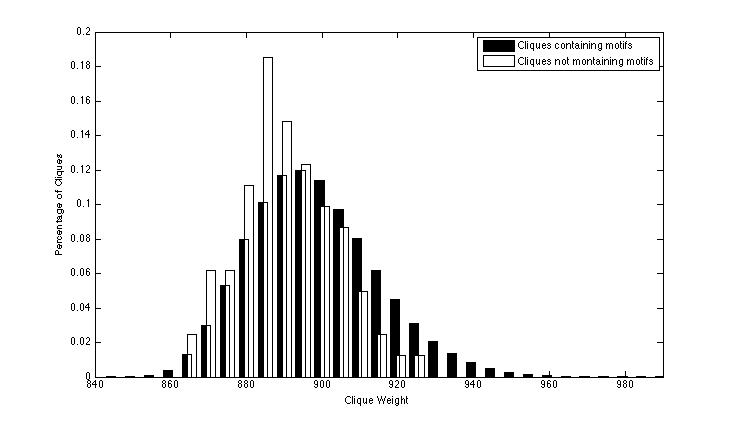
\includegraphics[width=170mm]{images/fig1}
%\caption[Distribution of the weight of cliques]{Distribution of the weight of cliques containing a center string and the distribution of the weight of cliques not containing a center string.  The data for non-motif cliques was generated was generated by running MCL-WMR 100 times, calculating the total weight of the clique, and generating a histogram of these values. The data  is given for the (15,4) motif problem instance with $n = 15$.  }
%\label{fig1}
%\end{center}
%\end{figure}
 
We can compare this theoretical tail bound with the distribution of the values obtained from MCL-WMR. Figure \ref{chapter4:fig2} demonstrates that as the value of $n$ increases, the deviation of the weight of cliques corresponding to motifs will occur with less probability, and the weight of the cliques will become more centralized around the mean.  Similar experimental tests were completed to demonstrate the relationship between the weight of spurious cliques when $n = 15$ and when $n = 50$, specifically, we ran MCL-WMR 100 times with $m = 800$, $\ell = 15$, and $d = 4$ and determined cliques that did not correspond to valid motifs. We found no spurious cliques in the data sets when $n = 50$, agreeing with our intuition that very few spurious cliques occur randomly in the data set when $n$ becomes large. 

We note our confidence in MCL-WMR being able to detect cliques -- both spurious and those corresponding to motifs -- this is due to the accuracy in detecting the embedded motifs (see Section \ref{results} details concerning these experimental tests).  These results also suggest that when $n$ is relatively large we can be more certain that any cliques found correspond to valid motifs (an attribute that will be further explored in this thesis).  

\begin{figure}[h*]
\begin{center}
 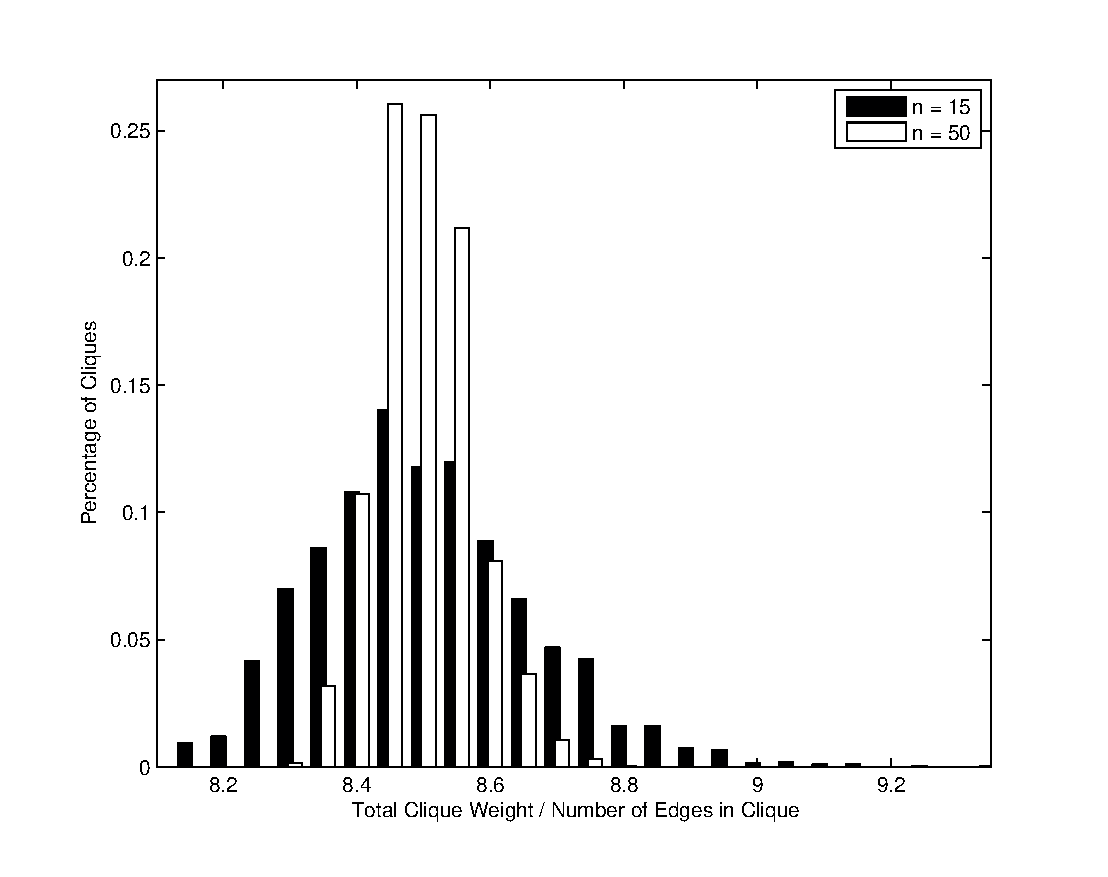
\includegraphics[width=\linewidth]{images/ex_n50a}
\caption[Data illustrating the distribution of the mean weight of an edge in a clique that corresponds to a valid motif set of size 15 and 50.]{Data illustrating the distribution of the mean weight of an edge in a clique that corresponds to a valid motif set  of size 15 (shown in black) and 50 (shown in white). The data is given for the $(15,4)$-motif problem with $m = 600$.  }
\label{chapter4:fig2}
\end{center}
\end{figure}

% Figure \ref{fig1} demonstrates that the distribution of the values of $W$ approach the normal distribution in the limit with the mean value entered at 897. This corresponds to the theoretical mean of 900.1 calculated using the result from Theorem \ref{mean_thm}.  Similarly, the weight of cliques that do not represent valid motifs follow a normal distribution, but the mean weight is approximately 885. This result, shown in Figure \ref{fig1}, was determined by generating the weight of the cliques that do not correspond to motifs in 100 random data sets , using MCL-WMR they are likely are not an uniform sample of all such cliques. 

\subsection{Discussion of Complexity}

A few interesting observations can be made regarding the complexity of the algorithm and the quality of its solutions. Finding cliques of maximum size in a given input graph is NP-complete and thus, unlikely to be solved in polynomial-time \cite{GJ}. Further, the results from Chen {\em et al.}\ \cite{CHKX04} show that unless unlikely consequences occur in parameterized complexity theory, the problem of finding maximum -- size cliques cannot be solved in $n^{o(k)}$ time. Thus, of finding cliques of size $k$ is not likely to be computationally feasible for graphs of significant size.  The best known algorithm for finding cliques of size $k$ in a given input graph runs in time $O(n^{ck/3})$, where $c$ is the exponent on the time bound for multiplying two integer $n \times n$ matrices; the best known value for is $c$ is 2.38 \cite{N02}.  

The running time for the straightforward algorithm that checks all size $k$ subsets is $O(n^{k+2})$ and is the one to be most likely to be implemented in practice.   The running time of the algorithm of  Yang and Rajapakse \cite{YR04}, a dynamic programming clique finding algorithm, is $O(n(mA^2 + A^{m - 1} p^{2m - 5})$, where $A = n \sum^{2d}_{i = 0}{{\ell}\choose i}(3/4)^i(1/4)^{\ell - i}$, $n$ is the length of each sequence and $m$ is the number of sequences.  This running time reflects the steep computational expense required to find cliques of a given size for an input graph.  Similarly, the estimated running time of the WINNOWER algorithm is $O((n D)^4)$, where $D$ is approximately $30$ for the challenge problem \cite{PS00}.  
 
The time required by MCL-WMR to find a solution is not affected directly by the length of the motif that is to be discovered, as is true of many other methods.  Rather, it is the weakness of the motif -- that is, the probability of the pairwise motif similarity occurring randomly -- that has the most impact on the complexity of the algorithm; the increased probability of a clique of high weight affects the running time of MCL-WMR since the exponential-time algorithm required to determine in a high cluster or subgraph contains a motif instance. 

We can compare the computational complexity of these programs by considering the required running time of MCL-WMR of the three sequential steps--that is, the computational time required to construct the graph, finds all cliques of size $n$, and determine the motifs and center string.  Other graphical methods of motif finding rely on an enumeration method to find dense subgraphs, including WINNOWER that requires each edge to be checked, and the algorithm of Yang and Rajapakse that uses dynamic programming on the complete graph. MCL-WMR omits this computational intensive work by employing MCL, which runs in time $O(N^3)$, where $N$ is the number of vertices of the input graph \cite{vD00}.  Hence, the most computationally expensive step is the clique-finding function, whose computation time increases with the number of vertices.

\section{Experimental Results}

We tested MCL-WMR on synthetic problem instances generated according to the embedded $(\ell, d)$-motif model. We produce problem instances as follows: first we choose a random string of length $\ell$, and pick $m$ occurrences of the motif by randomly choosing $d$ positions per occurrence and randomly mutating the base at each.  Lastly, we construct $m$ background sequences of length $n$ and insert the generated motifs into a random position in the sequence.  For each of the $(\ell,d)$ combinations, 100 randomly generated sets of input sequences ($n = 20$, $m = 600$) were generated.  An entry ``-'' indicates that the program was unable to solve the specific problem in a reasonable amount of time.
 
Our program found the exact location of a motif instance every single time and therefore, the performance coefficient is 1.  Other programs we tested did not achieve a performance coefficient of 1 and thus, returned approximate solutions to the embedded motif. The computation time of previous programs that find the exact solution becomes unacceptable as the motifs become degraded beyond the $(15,4)$ problem \cite{SJ04}.  For example, in 2004 Styczyski {\em et al.}\ \cite{SJ04} solved the $(17,5)$ problem exactly but took  greater than 3 weeks to do so and similarly, solving the $(14,4)$ took longer than 3 months (when $n = 20$ and $m = 600$).  The main advantage to our tool is the ability to solve the extremely difficult challenge problems (see Table \ref{performance1}).  See Subsection \ref{challenge_problems_section} for description of the term ``challenge problem''.


\begin{table}[h]
\begin{center}
\begin{tabular}{|c|c|c|c|c|c|c|}
\hline
$(\ell, d)$ & Gibbs & PROJECTION & SP-STAR & WINNOWER & MCL-WMR  \\
\hline 
(10, 2) & 0.150 & 0.80 & 0.56 & 0.78 & 1.00\\
(11, 2) & 0.68 & 0.94 & 0.84 & 0.90 & 1.00 \\
(12, 3) & 0.03 & 0.77 & 0.33 & 0.78 & 1.00 \\
(13, 3) & 0.60 & 0.94 & 0.92 & 0.92 & 1.00 \\
(14, 4) & 0.02 & 0.71 & 0.02 & 0.02 & 1.00  \\
(15, 4) & 0.19 & 0.93 & 0.73 & 0.92 & 1.00  \\
(17, 5) & 0.158 & 0.93 & 0.69 & 0.03 & 1.00 \\
(18, 6) & - & - & - & - &  1.00  \\
\hline
\end{tabular} 
\end{center}
\caption[Comparison of accuracy of MCL-WMR to other well-known motif-recognition programs on several challenge problems.]{Comparison of the performance on a range of $(\ell,d)$-motif problems with synthetic data.  Data from other algorithms are from Buhler and Tompa \cite{BT02}.  MCL-WMR, GibbsDNA, WINNOWER, and SP-STAR are averaged over eight random instances, while PROJECTION is averaged over 100 random instances.  In all these examples, $n = 20$ and $m = 600$.  }
\label{performance1}
\end{table} 


\begin{table}[h!]{
\begin{center}
\begin{tabular}{|c|c|c|}
\hline
$m$ & PROJECTION &  MCL-WMR\\
\hline 
600 & 2410 / 102  			& 2208 / 34 \\
800 & 2662 / 121			& 2802 / 42 \\
1000 & 2819 / 131			& 3223 / 89 \\
1200 & 3404 / 139 			& 3823 / 102\\
1400 & 3808 / 154 			& 4038 / 150 \\
1600 & 4310 / 159 			& 5037 / 167 \\
1800 & 4861 /  167 		& 4502 / 182 \\
2000 & 5012 / 182 			& 5001 / 201 \\
\hline
\end{tabular} 
\end{center}}
\caption[Comparison of the time required by MCL-WMR and PROJECTION to solve the $(15, 4)$-motif problem with 20 sequences of varying length.]{Comparison of the time required by MCL-WMR and PROJECTION to solve the $(15,4)$-motif problem with 20 sequences and $m$ varying between 600 to 2000.  The mean and standard deviation of the running time in CPU seconds is given. The success rate for PROJECTION was between 0.80 and 0.88.}
\label{n_table}
\end{table} 

The performance coefficient, which are shown for the various programs tested in Tables \ref{performance1}, \ref{n_table}, and \ref{performance2}, describe the fraction of  correctly solved instances and is described previously Subsection \ref{approximate_solution_section}. The performance coefficient of MCL-WMR is greater than that of the previous algorithms in every line of Table \ref{performance1}.  MCL-WMR correctly solved planted $(11,2)$, $(13,3)$, $(15,4)$, $(17,5)$ and $(18,6)$ on all data sets -- in these cases, the planted motif and motif occurrences at least as strong as planted motifs. WINNOWER, PROJECTION, and SP-STAR achieve acceptable performance on the $(11,2)$, $(13,3)$ and $(15,4)$ problem instances when the sequence length is less than or equal to 600 and the number of sequences is less than or equal to 20. However, all fail on the $(18,6)$ and $(19,6)$ problem, and WINNOWER and SP-STAR fail on the $(16,5)$ and $(17,5)$ problem instances.  The performance of MCL-WMR is best on the more difficult planted $(14,4)$, $(16,5)$, $(17,5)$ and $(18,6)$ motif problems when compared to results from previous algorithms.  WINNOWER and SP-STAR typically failed to find the planted motifs and PROJECTION often failed to have acceptable performance on the more difficult cases of the challenge problem \cite{BT02} and hence, MCL-WMR's performance substantially exceeded that of previously algorithms. 

We evaluated the performance of MCL-WMR on problem instances with longer background sequences -- that is, problems where $m$ varies from values greater than 600. As the length of the sequences increase, the number of randomly occurring $\ell$-mers increases; specifically, the increase in $m$ increases the probability of cliques of high-weight occurring. MCL-WMR will recover more computation time since the graph size will increase with the size of $m$.  Our results demonstrate that the computation time is comparable to that of PROJECTION, however, MCL-WMR is significantly more accurate than PROJECTION.  See Table \ref{n_table} for an illustration of these results.  Considering the $(15,4)$ motif problem and fixing the number of sequences to be 8, CONSENSUS, GibsDNA, and MEME have an unacceptable performance rate ({\em i.e.}\ below 0.7) when the sequence length increases to 300 or 400, the performance of WINNOWER breaks at length 700, and SP-STAR breaks when the length is 800 to 900. 
 
\begin{table}[h!]
\begin{center}
\begin{tabular}{|c|c|c|}
\hline
$(\ell, d)$ 	& PROJECTION 					& MCL-WMR  \\
\hline 
(10, 2) 			& 400 / 38	(0.98)			& 687 / 32 \\
(11, 2) 			& 670 / 43	(0.98)			& 1023 / 34 \\
(12, 3) 			& 1020 / 83 (0.87)			& 1442 / 52 \\
(14, 4) 			& 1521 / 95 (0.88)			& 1623 / 78 \\
(17, 5) 			& 5242 / 132 (0.78)			& 3023 / 103 \\
(18, 6) 			& -									& 5132 / 120 \\
\hline
\end{tabular} 
\end{center}
\caption[Comparson of the time required by MCL-WMR to PROJECTION to various motif challenge problems.]{Comparson of the running time of MCL-WMR to PROJECTION on various motif challenge problems. In all these examples, $n = 20$ and $m = 600$.  The mean and standard deviation of the running time in CPU seconds is given.  The success rate for PROJECTION is included in brackets. }
\label{performance2}
\end{table} 
\label{results}

	
\section{Summary and Open Problems}

We proposed an efficient algorithm for motif-recognition, whose specific purpose is to solve instances where there exists a large amount of degeneration with respect to the motif length.  We demonstrated promising results on synthetic data.  Specifically, we showed promising running time and accuracy for all challenge problems, with most-impressive improvement on the $(14,4)$, $(17,5)$ and $(18,6)$ problems.  Previous algorithms lack accuracy and efficiency in solving all challenge problems.  

Most importantly, we gave a novel model and framework for solving motif recognition instances that we will consider and study further in this thesis.  By changing the graphical model to incorporate edge weights, we can exploit theoretical results demonstrating the existence of a separation between the weights of cliques corresponding to valid motifs and the weights of those that do not, and obtain improved search techniques.   Our theoretical work and empirical data show a large percentage of the cliques corresponding to valid motifs have total weight in a narrow range.  This helps us distinguish cliques containing valid motifs and spurious cliques.  

The largest area for further improvement of MCL-WMR is the recovery of the motifs.  The dynamic-programming algorithm that explores the dense subgraphs to determine which subgraphs correspond to motif sets, and which correspond to decoy sets requires exponential time.  Note that this deciphering of subgraphs essentially reduces to solving instances of the {\sc Closest String} problem.  Next, we aim to create, analyze, and employ efficient algorithms for the {\sc Closest String} problem.  

%======================================================================
\chapter{Algorithms and Analysis for the {\sc Closest String} Problem}\label{chapter:closest_string_problem}
%======================================================================

In the previous chapter we described MCL-WMR, a motif-recognition program that builds a weighted graph model of the input data, efficiently clusters the data to determine smaller subproblems that are likely to contain a motif, and recovers motifs by the use of a dynamic-programming algorithm.  The last step involves solving the {\sc Closest String} problem a significantly large number of times.  As described in the previous chapter, we refer to a set of strings $S$ as pairwise bounded if for all strings $a, b \in S$, $d(a,b) \leq 2d$.  Thus, the {\sc Closest String} problem reduces to discerning between pairwise bounded sets that have a center string, and if so, finding one such string $s^*$, and those sets that do not. The dynamic-programming algorithm used by MCL-WMR to solve the {\sc Closest String} problem has exponential running time and in practice is the most computational intensive step of MCL-WMR. Hence, this algorithm becomes a significant bottleneck in solving motif-recognition instances -- especially where $d$ is large relative to $\ell$. To improve upon the capability of MCL-WMR, we develop efficient heuristics to solve the {\sc Closest String} problem.  

In this chapter we study the {\sc Closest String} problem in more detail.  Smith showed several results indicating the ``alphabet size does significantly influence many pattern finding problems''  \cite[p. 51]{asmith}.   Similarly, we give strong evidence to demonstrate that the number of strings has a significant affect on the cost of solving the {\sc Closest String} problem and therefore, influences how we should attempt to solve the problem.  We investigate different methods for efficiently discerning between motif sets and decoy sets; to accomplish this task we will divide the problem into studying instances with a small number of strings, and instances with a large number of strings. 
  
Following the path of previous authors \cite{GNR01,SLC04}, we first focus on efficiently solving restricted instances of the {\sc Closest String} problem. Gramm {\em et al.}\ \cite{GNR01}  and Sze {\em et al.}\ \cite{SLC04}  gave direct, combinatorial algorithms for solving the {\sc Closest String} problem exactly for three strings.  The algorithm of the former authors considers the possible combinations of alphabet symbols that can occur for three strings, then specifies conditions for which a center string can be constructed \cite{GNR01}.  Sze {\em et al.}\ \cite{SLC04} gave a counting argument to demonstrate a condition for which a set of three strings has a center string and when it does not.  Gramm {\em et al.}\ stated that the problem of finding an efficient polynomial-time algorithm for solving the {\sc Closest String} problem on a set of four strings remains open ``due to the enormous combinatorial complexity [of the integer linear programming based solution]'' \cite[p. 13]{GNR03}.  We resolve this open problem for binary strings; specifically, we give an exact combinatorial algorithm for four binary strings.  

We also prove that {\sc Closest String} instances can be solved efficiently when the instances have a large number of strings.  Evidence for the efficiency is provided in a two-fold manner.  First, we introduce and investigate a randomized algorithm for the {\sc Closest String} problems, which we refer to as {\em CSP-Greedy}.  We prove that this randomized algorithm computes, with high probability, the {\sc Closest String} on smoothed instances up to a constant factor approximation.  Using smoothed analysis, we show the algorithm runs in $O(\ell^3)$, where $\ell$ is the string length, and achieves a $(1 + f(\epsilon, n, \ell))$ approximation guarantee, where $\epsilon > 0$ is any small value, $n$ is the number of strings, and $f(\epsilon, n, \ell) = O(\delta^n) $ for some $\delta < 1$.  

Next, we examine the $O(n\ell + nd \cdot d^d)$-time algorithm by Gramm {\em et al.}\ \cite{GNR03}, which has been shown to work very efficiently on practical instances. We explain this good performance through smoothed analysis.  Essential to our analysis is the introduction of a new perturbation model of the {\sc Closest String} model and the analysis of the Gramm {\em et al.}\ \cite{GNR03} algorithm in this model. We prove for any given {\sc Closest String} instance $I$, the average running time of this algorithm on a small perturbation of $I$ is $O(n\ell + nd \cdot d^{2 - \epsilon})$.  

We refer to the {\em cardinality} of a {\sc Closest String} instance as the number of strings in the set.  We note that the results in this chapter are complementary; the first part of this chapter will demonstrate that small, very restricted instances can be solved efficiently and the second part will show that instances that contain a large number of strings can be solved efficiently.   
 
We conclude this section by showing the applicability of this analysis to motif recognition. We extend MCL-WMR to incorporate {\em CSP-Greedy} and obtain {\em pMCL-WMR}, a program that is able to detect motifs in sets of large cardinality ({\em i.e.} instances that have 30 or more sequences) and find regulatory sequences in genomic data.  Our data shows that detecting motifs in large data sets is easier in comparison to when the number of sequences is relatively small -- a fact that gives surprising insight into this central problem in bioinformatics. 

\newpage
The main contributions in this chapter are as follows:
\begin{itemize} 
\item We give a linear-time algorithm for solving small {\sc Closest String} instances (Section \ref{sec:small_CS_insances}).
\item We describe our algorithm, {\em CSP-Greedy}, prove it achieves a 2-approximation guarantee, and give a bound on the probability that {\em CSP-Greedy} returns an optimal solution to the {\sc Closest String} instance.  Using smoothed analysis we show {\em CSP-Greedy} achieves an $1 + f(\epsilon, n, \ell)$-approximation guarantee in time $O(\ell^3)$, where $\epsilon > 0$ is any small value and $f(\epsilon, n, \ell)$ approaches zero in time that is exponential in $n$, and the expected running time of the algorithm of Gramm {\em et al.}\ \cite{GNR03} is $O(n\ell + nd \cdot d^{2 + \epsilon})$ (Section \ref{sec:large_CS_insances_v1}).
\item We show the applicability of the algorithms for solving {\sc Closest String} instances in speeding up motif detection (Section \ref{section:exp_results}).
\end{itemize}

%%%%%%%%%%%%%%%%%%%%%%%%%%%%%%%%%%%%%%%%%%%%%%%
\section{A Linear-Time Algorithm for Solving Small \\ {\sc Closest String} Instances} \label{sec:small_CS_insances}

In this section, we provide empirical evidence suggesting that the majority of decoy sets have a subset of cardinality four that is a decoy, and describe a linear-time algorithm for determining whether a set of four strings is a decoy, addressing an open problem of Gramm {\em et al.}\ \cite{GNR03}. Our empirical results together with our algorithm suggest that the majority of instances of the {\sc Closest String} problem can be solved in polynomial time.

We begin with some definitions concerning general string analysis.  Let $\ell$, $d$, and $n$ be positive integers with $d \leq \ell$. Let $\sigma_i$ be a function that returns the $i$th symbol in a string. For any symbol $\beta \in \Sigma$ let $\beta^{\ell}$ denote the length $\ell$ string of all $\beta$ symbols. Given a set of strings $S = \{ s_1, \ldots, s_n \}$, each of which has length $\ell$, the $i$th {\em column} refers to the column vector $c_i = [\sigma_i(s_1), \ldots, \sigma_i(s_n)]^T$ in the $n \times \ell$ matrix representation of $S$. 

We will be interested in the cardinality of a decoy set, that is, the number of strings contained in the set. We say set $\hat{S} \subseteq S$ is a decoy of {\em minimal cardinality} if $\hat{S}$ is a decoy set such that for all $S' \subseteq S$, if $|S'| < |\hat{S}|$, then $S'$ has a center string. 


Gramm {\em et al.}\ \cite{GNR01} refer to the process of permuting the columns of $S$ such that these are grouped by column type as {\em normalization}. A normalized instance can be derived from the input set of strings by a simple linear-time algorithm.  Given a {\sc Closest String} for the normalized set of strings, the inverse of this same permutation returns
a center string for the original input \cite{GNR01}. 

\subsection{Definitions Specific to Sets of Cardinality Four}
 
Given a binary alphabet $\Sigma = \{\alpha, \beta \}$ and a set of strings $S=\{s_1, \ldots, s_4\}$, the symbols in each column have  either two, three, or four matching symbols. Sixteen types of columns are possible in general. We say a column belongs to {\em group $i$} if it has exactly $i$ matching symbols. To reduce the number of possible types to eight, suppose without loss of generality that $s_4 = \beta^{\ell}$. Equivalently, create a new set $S'$ by performing a logical exclusive-or of each string in $S$ with $s_4$ (say $\alpha$ corresponds to boolean true). A center string for $S$ is found by performing another exclusive-or on a center string for $S'$. Let $\lambda_{abc}$ denote the number of instances of column  $(a, b, c, \beta)^T$, where $a, b, c \in \{\alpha, \beta \}$. See Table~\ref{tab:possible_columns}. Note that only columns of groups three and two need to be considered, since any center string will correspond to the majority at each column of group four.  A pair of columns are considered to be {\em identical} if a pair of strings in one column mismatch if and only if the same strings mismatch in the second column.  For example the column $[  \alpha \alpha \beta \beta ]^T$ is identical to $[\beta \beta \alpha \alpha]^T$, but neither is identical to $[\alpha \beta \beta \alpha]^T$.  

Let $\maj_i$ denote the majority of the four symbols in column $i$. That is, $\maj_i = \alpha$ if symbol $\alpha$ occurs three or more times in column $i$ and $\maj_i = \beta$ if symbol $\beta$ occurs three or more times; $\maj_i$ is undefined if $\alpha$ and $\beta$ each occur twice.  Assuming that $s_4 = \beta^{\ell}$, only the columns associated with $\lambda_{\alpha\alpha\alpha}$ are such that $\maj_i = \alpha$.

\begin{table}[t]
\begin{center}
%\begin{tabular*}{0.75\textwidth}{@{\extracolsep{\fill}}|c|c|cccc|ccc|}
\begin{tabular}{|c|c|cccc|ccc|}
\hline
Group & 
\multicolumn{1}{c|}{Four} &
\multicolumn{4}{c|}{Three} &
\multicolumn{3}{c|}{Two} \\
\hline
\# of columns. &  $\lambda_{\beta\beta\beta}$ & $\lambda_{\alpha\beta\beta}$ & $\lambda_{\beta\alpha\beta}$ & $\lambda_{\beta\beta\alpha}$ & $\lambda_{\alpha\alpha\alpha}$ & $\lambda_{\beta\alpha\alpha}$ & $\lambda_{\alpha\beta\alpha}$ &   $\lambda_{\alpha\alpha\beta}$\\
\hline
$s_1$ 		& $\beta$ & $\alpha$ & $\beta$ & $\beta$ & $\alpha$ & $\beta$ & $\alpha$ & $\alpha$ \\
$s_2$ 		& $\beta$ & $\beta$ & $\alpha$ & $\beta$ & $\alpha$ & $\alpha$ & $\beta$ & $\alpha$ \\
$s_3$ 		& $\beta$ & $\beta$ & $\beta$ & $\alpha$ & $\alpha$ & $\alpha$ & $\alpha$ & $\beta$ \\
$s_4$ 		& $\beta$ & $\beta$ & $\beta$ & $\beta$ & $\beta$ & $\beta$ & $\beta$ & $\beta$ \\
\hline
$\maj_i$ & $\beta$ & $\beta$ & $\beta$& $\beta$ & $\alpha$ & - & - & - \\
\hline
\end{tabular}
\caption[Defining the different types of columns for a set of strings with cardinality four.]{Defining the different types of columns for a set of strings with cardinality four. The values $\lambda_{\alpha\beta\beta}$ through $\lambda_{\alpha\alpha\beta}$ denote the number of columns of each type in
groups three and two.  The symbol ``-'' implies that the value is undefined at these columns.}
\end{center}
\label{tab:possible_columns}
\end{table}

%%%%%%%%%%%%%%%%%%%%%%%%%%%%%%%%%%%%%%%%%%%%%%%%%%%%%%%%%%%%%%%%%%%%%%%%%%%%%%%%%%%%%%%%%%%%%%%%%%%%%%%%%%%%%%%%%% 
\subsection{Ubiquitousness or Rarity of Bounded Decoy Sets}

We consider the relative frequency, or infrequency, of decoy sets that do not have a proper subset that is also a decoy. Our empirical results demonstrate that the relative frequency of such decoy sets is minimal, and that the majority of decoy sets contain a decoy subset of cardinality four.  Still, the results of Gramm {\em et al.}\ \cite{GNR03} imply that we cannot characterize all decoy sets of arbitrary size $n$ as having a proper subset that is a decoy. We refer to a set $Q$ of decoys, each of cardinality $n$,  as having decoys of {\em bounded cardinality} if every decoy in $Q$ has a proper subset that is a decoy.
  
\begin{proposition} \label{cb1:corollary1} Let $\Sigma$ denote an alphabet of arbitrary fixed size. If $P \neq NP$, then for any $n_0$ there exists a decoy set $S$ such that every subset of $S$ of cardinality $n_0$ has a center string. \end{proposition}

\begin{proof} Suppose otherwise. That is, there exists an $n_0$ such that
every decoy $S$ of size $n \geq n_0$
has a subset of size $n_0$ that is a decoy.
By Gramm {\em et al.}\ \cite{GNR03}, for any fixed $n_0$, 
there exists an algorithm that decides whether a set of $n_0$ strings 
is a decoy in $f(\ell,d)$ time, where $f(\ell,d)$ is polynomial in $\ell$ and $d$.
Consequently, for any set of $n \geq n_0$ strings $S$, 
we can check each of the ${{n} \choose {n_0}}$ subsets of $S$ of size $n_0$
to determine whether any is a decoy in time $O(n^{n_0} f(l,d)))$.
That is, we can determine in polynomial time whether $S$ is a decoy.
Since the {\sc Closest String} problem is NP-complete, 
this is possible only if P = NP.
\hfill $\Box$ \end{proof}

It should be noted that Proposition \ref{cb1:corollary1} does not preclude that there may exist values of $n$ such that all decoys of cardinality $n$ have a minimal decoy set of cardinality $n$.  Proposition \ref{cb1:corollary1}  implies that there does not exist a threshold $n_0$ such that every decoy set contains a minimal decoy set of cardinality at most $n_0$, if $P \not= NP$.  Although Proposition~\ref{cb1:corollary1} implies that no fixed $n_0$ exists, we conjecture that most decoys have a subset of size four that is a decoy. We provide evidence toward this property with an empirical study on random sets of binary strings which we now describe. In turn, these results motivate the need for an efficient algorithm for determining whether a set of four strings has a center string; we describe such an algorithm in Section~\ref{sec:alg}.

\begin{table}[th]
\begin{center} {\footnotesize
\begin{tabular}{|c||c|c|c||c|c|c||c|c|c|}
\hline
Number of 			& \multicolumn{3}{c||}{$\ell = 8$, $d = 3$} & \multicolumn{3}{c||}{$\ell = 10$, $d = 3$}  & \multicolumn{3}{c|}{$\ell = 15$, $d = 4$} \\
strings 	& \multicolumn{1}{c|}{$n = 6$} & \multicolumn{1}{c|}{$n = 10$} & \multicolumn{1}{c||}{$n = 12$} 
					& \multicolumn{1}{c|}{$n = 6$} & \multicolumn{1}{c|}{$n = 10$} & \multicolumn{1}{c||}{$n = 12$}  
    				& \multicolumn{1}{c|}{$n = 6$} & \multicolumn{1}{c|}{$n = 10$} & \multicolumn{1}{c||}{$n = 12$} \\
\hline
\hline
No. of valid &	443.4	&	4.6 &	88.7 &	394.4 & 9.3 & 3.6 & 101.4 & 3.5 & 2.6 \\
motif &&&&&&&&& \\
\hline
\hline
 4 		& 542.2    & 995.4  	& 991.3  	& 605.6 	& 990.7 	&  996.4 		& 898.6 	& 996.5 	&  997.4  	\\
 5  		& 12.4     	& 0 			& 0   	 	& 7  			&  0  		&  0 				& 4.1  		&  0  		&  0 	\\
 6 		& 2     		& 0   		& 0 			& 0.2  		&  0 			&  0  			& 0.8  		&  0 			&  0  \\
 7    		& -     		& 0   		& 0  			& -  			&  0 			&  0 				& -  			&  0 			&  0 	\\
 8  		& -     		& 0   		& 0  			& -  			&  0 			&  0 				& -  			&  0 			&  0	\\	
 9   		& -     		& 0   		& 0  			& -  			&  0 			&  0 				& -  			&  0 			&  0	\\	
 10    	& -     		& 0  			& 0   		& -  			&  0 			&  0 				& -  			&  0  		&  0	\\
 11    	& -     		& -  			& 0   		& -  			&  -			&  0 				& -  			&  - 			&  0	\\
 12       & -     		& -  			& 0  			& -  			&  -			&  0    			& -  			&  - 			&  0	\\
\hline
\end{tabular} }
\end{center}
\caption[Experimental data illustrating the ubiquitousness of decoy sets of cardinality four.]{Experimental data illustrating the ubiquitousness of decoy sets of cardinality four. Data obtained from calculating the average of 10 experiments that obtain a random sample, without replacement, of 1000 sets of strings and determining the size of the minimal decoy contained in each set decoy obtained in the sample.  The first column is the cardinality of the minimum decoy set. }
\label{decoy_table}
\end{table} 

We empirically investigate the rarity of the occurrence of decoy sets of cardinality $n$ for which the cardinality of a minimal decoy set is large relative to $n$. We sampled without replacement 1000 times from the set of all possible pairwise-bounded sets of binary, length-$\ell$ strings; each set sampled has exactly $n$ strings taken from the binary alphabet.  We varied the values for $n$, $\ell$ and $d$.  For each sample set, we determined whether the set is a decoy or a valid motif, with respect to the value of $d$, and determined the cardinality of the minimum decoy set.  We repeated this experiment ten times and calculated the mean values obtained. Table \ref{decoy_table} outlines this data. One significant empirical trend demonstrates that as the number of strings increased, the number of decoys that do not contain a minimal decoy of cardinality four became exponentially smaller; when $n$ was ten and twelve the number of minimal decoys of size larger than four was zero.  The only value of $n$ for which decoys of size $n$ were seen was six.  Further, the total number of decoys in 900,000 sets of strings sampled was approximately 1,500.  In summary, the empirical results suggest that a large percentage of binary decoys can be characterized by containing a minimal decoy set of size four, the smallest size possible, further motivating the main results in the following subsection.  

\subsection{Finding a Center String for a Set of Four Strings} \label{sec:alg}
 
The only previous polynomial-time solution for finding a center string of a set of four strings was intended more to demonstrate the fixed-parameterized tractability of the problem rather than to provide an efficient solution \cite{GNR03}. As acknowledged by its authors, the corresponding description (for which many details are omitted) results in an algorithm with extremely high  (although theoretically linear) run time and, furthermore, does not lend itself well to simple or practical implementation. We present a simple linear-time algorithm for finding a center string of a set of four binary strings or determining that the set is a decoy. After describing the algorithm, we prove its correctness and  show its worst-case run time is $O(\ell)$ for any arbitrary $d$.

Given a set of binary strings $S = \{s_1, \ldots, s_4\}$,  algorithm {\sc BinaryClosestString4}  identifies a center string $s^*$ for $S$ if one exists. Again, to simplify the algorithm's description, suppose $s_4 = \beta^{\ell}$. The algorithm greedily assigns symbols to $s^*$, one symbol at a time. Each column $c_i$ is initially considered to be {\em free};
that is, no symbol has been assigned to $\sigma_i(s^*)$. Once it is assigned a symbol, we say column $c_i$ is {\em fixed} and its value is not modified again.
%The first four values in a column may have either two, three, or four matching 
%symbols.
%We say a column belongs to group $i$ if it has exactly $i$ matching symbols. 
%Eight types of columns are possible. 
%Let $\lambda_{\beta\beta\beta}$ through $\lambda_{\alpha\alpha\beta}$ 
%denote the respective number of columns of each type.
%See Table~\ref{tab:phase3}.
The algorithm has three phases in which columns of groups four, three, 
and two are fixed, respectively.

{\bf Phase One.}
Fix symbols of $s^*$ in all columns of group four such that these agree with 
the symbol of the corresponding column.

{\bf Phase Two.}
The symbols of $s^*$ in columns of group three are fixed sequentially. 
Say the first $i-1$ columns of group three have been fixed and consider the $i$th such column.
Let $s_j$ denote the string in $S$ that disagrees with the
remaining three strings in this column.
Let $s^+$ denote the string 
given by the symbols of $s^*$ in the fixed columns 
and the symbols of $s_j$ in the free columns.
If $s^+$ is a center string for $S$, then let $s^* = s^+$ and return $s^*$.
Otherwise, fix the current column of $s^*$ to agree with the majority
and continue to the next column of group three.

{\bf Phase Three.}
If phase three is reached, then only columns of group two remain,
of which at most three types may be present.
The free columns are fixed by selecting the number of columns
of each type that will be assigned symbol $\alpha$ versus $\beta$.
That is, a solution for columns of group two corresponds to a triple of integers
$(x,y,z)$,
where $x \in [0,\lambda_{\beta\alpha\alpha}]$
denotes the number of columns of type $\lambda_{\beta\alpha\alpha}$
that will be assigned the symbol $\alpha$ 
and $\lambda_{\beta\alpha\alpha}-x$ represents the number that will 
be assigned the symbol $\beta$.
The variables $y$ and $z$ are defined analogously.
See Table~\ref{tab:phase3}.
We denote the corresponding string by $s^*_{x,y,z}$.
Therefore, the problem reduces to identifying an integer triple $(x,y,z)$
selected from the region $R = [0, \lambda_{\beta\alpha\alpha}]
\times [0, \lambda_{\alpha\beta\alpha}] 
\times [0, \lambda_{\alpha\alpha\beta}]$
that minimizes
\begin{equation}
\label{eqn:minimizeObj}
f(x,y,z) = \max_{s_i \in S} d(s_i, s^*_{x,y,z}) ,
\end{equation}
where
\begin{subequations}
\begin{align}
d(s_1, s^*) & = \lambda_{\alpha\beta\beta} + x + \lambda_{\alpha\beta\alpha} - y
+ \lambda_{\alpha\alpha\beta} - z , 
\label{eqn:phase3Constraint1}
\\
d(s_2, s^*) & = \lambda_{\beta\alpha\beta} + \lambda_{\beta\alpha\alpha} - x 
+ y + \lambda_{\alpha\alpha\beta} - z , 
\label{eqn:phase3Constraint2}
\\
d(s_3, s^*) & = \lambda_{\beta\beta\alpha} + \lambda_{\beta\alpha\alpha} - x 
+ \lambda_{\alpha\beta\alpha} - y + z , 
\label{eqn:phase3Constraint3}
\\
d(s_4, s^*) & = \lambda_{\alpha\alpha\alpha} + x + y + z .
\label{eqn:phase3Constraint4}
\end{align}
\end{subequations}
The string $s^*_{x,y,z}$ does not actually need to be constructed since
the corresponding value of \eqref{eqn:minimizeObj} is obtained in constant time
upon fixing values for $x$, $y$, and $z$.

\begin{table}
\centering
%\begin{tabular*}{0.75\textwidth}{@{\extracolsep{\fill}}|cc|c|cccc|ccc|}
\begin{tabular}{|cc|c|cccc|ccc|}
\hline
\multicolumn{2}{|r|}{Column Group} &
\multicolumn{1}{c|}{Four} &
\multicolumn{4}{c|}{Three} &
\multicolumn{3}{c|}{Two} \\
\multicolumn{2}{|r|}{Algorithm Phase} &
\multicolumn{1}{c|}{1} &
\multicolumn{4}{c|}{2} &
\multicolumn{3}{c|}{3} \\
\hline
\multicolumn{2}{|r|}{Number of Columns} &
$\lambda_{\beta\beta\beta}$ &
$\lambda_{\alpha\beta\beta}$ &
$\lambda_{\beta\alpha\beta}$ &
$\lambda_{\beta\beta\alpha}$ &
$\lambda_{\alpha\alpha\alpha}$ &
$\lambda_{\beta\alpha\alpha}$ &
$\lambda_{\alpha\beta\alpha}$ &
$\lambda_{\alpha\alpha\beta}$ \\
%used to be & & & a & b & c & d & e & f & g \\
\hline
\multirow{4}{*}{Set $S$} 
& $s_1$ & $\beta$ & $\alpha$ & $\beta$ & $\beta$ &
$\alpha$ & $\beta$ & $\alpha$ & $\alpha$ \\
& $s_2$ & $\beta$ & $\beta$ & $\alpha$ & $\beta$ &
$\alpha$ & $\alpha$ & $\beta$ & $\alpha$ \\
& $s_3$ & $\beta$ & $\beta$ & $\beta$ & $\alpha$ &
$\alpha$ & $\alpha$ & $\alpha$ & $\beta$ \\
& $s_4$ & $\beta$ & $\beta$ & $\beta$ & $\beta$ & 
$\beta$ & $\beta$ & $\beta$ & $\beta$ \\
\hline
Center string & $s^*$ & $\beta$ & $\beta$ & $\beta$ & $\beta$ & $\alpha$ &
$x$ & $y$ & $z$ \\
\hline
\end{tabular}
\caption[Illustration of the center string found by algorithm {\sc BinaryClosestString4}]{The center string found by algorithm {\sc BinaryClosestString4} 
(if one exists) is displayed in the last row. The center string is denoted as $s^*$.
The values $\lambda_{\beta\beta\beta}$ 
through $\lambda_{\alpha\alpha\beta}$ 
denote the number of columns of each type 
and functions $x$, $y$, and $z$ denote the number of occurrences of symbol
$\alpha$ in the corresponding column as derived by the algorithm.}
\label{tab:phase3}
\end{table}

Instead of evaluating all integer combinations for $(x,y,z)$
(requiring $O(\ell^3)$ time),
we identify a set $T \subseteq \mathbb{Q}^3 \cap R$ 
containing a constant number of triples
such that the optimal (possibly non-integer)
solution to \eqref{eqn:minimizeObj} is a triple in $T$.
Interpreted geometrically, 
\eqref{eqn:phase3Constraint1} through \eqref{eqn:phase3Constraint4}
correspond to four respective hyperplanes in $\mathbb{R}^4$
whose maximum, $f(x,y,z)$, defines a surface.
Let
\begin{align}
x_0 & = \frac{1}{4} \left(
- \lambda_{\alpha\beta\beta} + \lambda_{\beta\alpha\beta}
+ \lambda_{\beta\beta\alpha} - \lambda_{\alpha\alpha\alpha}
+ 2\lambda_{\beta\alpha\alpha} \right) ,
\nonumber \\
y_0 & = \frac{1}{4} \left(
  \lambda_{\alpha\beta\beta} - \lambda_{\beta\alpha\beta}
+ \lambda_{\beta\beta\alpha} - \lambda_{\alpha\alpha\alpha}
+ 2\lambda_{\alpha\beta\alpha} \right) ,
\nonumber \\
z_0 & = \frac{1}{4} \left(
  \lambda_{\alpha\beta\beta} + \lambda_{\beta\alpha\beta}
- \lambda_{\beta\beta\alpha} - \lambda_{\alpha\alpha\alpha}
+ 2\lambda_{\alpha\alpha\beta} \right) .
\label{eqn:phase3Sol}
\end{align}
If $(x_0,y_0,z_0) \in R$, then let $T = \{(x_0, y_0, z_0)\}$.
Otherwise, let $T$ denote the set of triples that correspond to
$x$-, $y$-, and $z$-coordinates of vertices of the
intersection of the surface defined by 
\eqref{eqn:minimizeObj} with the boundary of $R$.
If this intersection is empty, then it follows that no center string exists.

For each triple $(x,y,z) \in T$, 
evaluate the integer triples within unit $L_\infty$ distance 
of $(x,y,z)$ in region $R$. 
That is, for every $(x,y,z) \in T$, consider the integer triples in 
$[ \max(0, x-1), \min(x+1, \lambda_{\beta\alpha\alpha}) ]
\times [ \max(0, y-1), \min(y+1, \lambda_{\alpha\beta\alpha}) ]
\times [ \max(0, z-1), \min(z+1, \lambda_{\alpha\alpha\beta}) ]$,
of which there are at most eight.
Compute \eqref{eqn:minimizeObj}
for each such integer triple $(x,y,z)$
and store the corresponding minimizing string $s^*_{x,y,z}$.
Let $s^* = s^*_{x,y,z}$.

%If $x_0$ (respetively, $y_0$ or $z_0$) 
%lies outside the range of feasible solutions 
%$[0, \lambda_{\beta\alpha\alpha})]$, then $x_0$
%is assigned a new value corresponding to the nearest endpoint of that interval.
%For example, if $x_0 < 0$ then set $x_0 = 0$.
%As a result, the values of $y_0$ and $z_0$ are updated by one of four
%possible values, from which the optimum is selected.
%These four new potential points are found by solving
%for $t$ in each of the four sets of equations, depending on which of 
%$x_0$, $y_0$, or $z_0$ has a new fixed value.
%\begin{subequations}
%\begin{align}
%x_1(t) = t+\frac{1}{2}(-a+c+e-f)
%& y_1(t) = t+\frac{1}{2}(-b+c+e-g)
%& z_1(t) = t ,
%\\
%x_2(t) = -t+\frac{1}{2}(b-d+e+g)
%& y_2(t) = -t+\frac{1}{2}(a-d+f+g)
%& z_2(t) = t ,
%\\
%x_3(t) = t+\frac{1}{2}(-a+c+e-g)
%& y_3(t) = t+\frac{1}{2}(-a+c+e-g)
%& z_3(t) = t ,
%\\
%x_4(t) = -t+\frac{1}{2}(b-d+e+g)
%& y_4(t) = t+\frac{1}{2}(-b+c+f-g)
%& z_4(t) = t .
%\end{align}
%\end{subequations}
%
%The remaining optimization corresponds to a set of four planes in 
%$\mathbb{R}^3$. Again, the optimal solution lies at one of two vertices
%on the 1-level (maximum) surface.
%If the lower of these points lies outside $R$,
%the corresponding variable, say $y$ is truncated, and the search
%continues on a set of four lines in $\mathbb{R}$, for which the optimal
%solution lies at one of three vertices on the 1-level.
%Again, the optimal remaining varibles 
%then the best solution inside $R$

{\bf Termination.}
Consider the maximum distance between $s^*$ and a string in $S$,
{\em i.e.}, the minimum (integer) value of \eqref{eqn:minimizeObj}.
If this value is at most $d$, 
then $s^*$ is returned as a center string for $S$. 
Otherwise, $S$ is a decoy set and no center string exists.

We now demonstrate that algorithm {\sc BinaryConsensus4} correctly returns a 
center string $s^*$ for every set $S$ that is a valid motif set.
Furthermore, this is achieved in $O(\ell)$ time, independent of $d$.
The proof of Theorem~\ref{thm:algCorrectness} refers to 
Lemmas~\ref{lem:phase2} and~\ref{lem:phase3} which follow.

\begin{theorem}
\label{thm:algCorrectness}
Given any $d \in \mathbb{Z}^+$, any $\ell \in \mathbb{Z}^+$,
and any set $S$ of four binary strings of length $\ell$,
algorithm {\sc BinaryConsensus4} 
returns a center string for $S$ with degeneracy parameter $d$
if one exists or returns that $S$ is a decoy
in $O(\ell)$ time.
\end{theorem}

\begin{proof}
The correctness of Phase One is straightforward.
The correctness of Phase Two follows by induction on $i$ 
using Lemma~\ref{lem:phase2}.
Consequently, if $S$ has a center string, then either one has been found 
by the end of Phase Two (i.e., $s^* = s^+$), 
or there exists a center string $s^*$ such that
$\sigma_x(s^*) = \maj_x$ for all columns of groups three and four.
The optimal solution for the remaining free columns is found in Phase Three.
The correctness of Phase Three follows by Lemma~\ref{lem:phase3}.
Therefore, algorithm {\sc BinaryClosestString4} returns a center string $s^*$
if one exists, and returns that no center string exists otherwise.

Each phase requires a single pass through the columns of $S$.
Phase One simply requires counting the number of columns of each type.
Phase Two also requires maintaining the twelve distances $d(s_i, s^+_j)$
for each $\{i, j\} \subseteq \{1, \ldots, 4\}$, 
where $s^+_j$ denotes $s^+$ for which the free columns are
defined according to $s_j$ 
(as described in Phase Two of algorithm {\sc BinaryConsensus4}).
Every time a column of group three is fixed,
each of these twelve values can be updated in constant time.
Phase Three simply requires counting the number of columns of each type.
Since \eqref{eqn:minimizeObj} 
is defined by the maximum of four hyperplanes and
region $R$ is bounded by three pairs of parallel planes,
the number of triples in $T$ is constant and, furthermore, the coordinates
of these triples are straightforward to compute in constant time.
Finally, since any point in $\mathbb{R}^3$ has at most eight integer points 
within unit $L_\infty$ distance from it, the set of integer triples evaluated
is also computed in constant time and space.
Therefore, algorithm {\sc BinaryConsensus4} terminates in $O(\ell)$ time.
\hfill $\Box$ \end{proof}

\begin{definition}[Majority-Rule Property]
We say property $P(i)$ holds for a set $S$ of four binary strings 
if and only if either
\begin{enumerate}
\item $S$ is a decoy, or
\item there exists a center string for $S$ for which
the first $i$ columns of group three have value $\maj_i$.
\end{enumerate}
\end{definition}

\begin{lemma}
\label{lem:phase2}
Let $S = \{s_1, \ldots, s_4\}$ denote a set of four binary strings
that has $m$ columns of group three.
If $P(i)$ holds for some $i \in \{0, \ldots , m-1\}$ 
and $s_j \in S$ denotes the string that mismatches in the $(i+1)$st 
column of group three, then either
\begin{enumerate}
\item $P(i+1)$ holds for $S$, or
\item $s^+$ is a center string for $S$,
\end{enumerate}
where $\sigma_x(s^+) = \maj_x$ in the first $i$ columns of group three
and $\sigma_x(s^+) = \sigma_x(s_j)$ in the remaining columns.
\end{lemma}

\begin{proof}
If $s^+$ is a center string for $S$ then the claim holds.
Similarly, if $S$ is a decoy then $P(i+1)$ is true and the claim holds.
Therefore, suppose $S$ is not a decoy and $s^+$ is not a center string for $S$.
By $P(i)$, $S$ has a center string $s^*$ 
for which the first $i$ columns of group three have value $\maj_x$.
Let $k$ denote the index of the $(i+1)$st column of group three.

{\it Case 1.} 
Suppose $\sigma_k(s^*) = \maj_k$.
Therefore, $P(i+1)$ is true, and the claim holds.

{\it Case 2.} 
Suppose $\sigma_k(s^*) \neq \maj_k$. That is, $\sigma_k(s^*) = \sigma_k(s_j)$.
Since $s^+$ is not a center string, 
$s^*$ and $s^+$ must differ in at least one column; 
let $k'$ denote the index of such a column.
Let $s^{**}$ denote a string of length $\ell$ 
such that $\sigma_x(s^{**}) \neq \sigma_x(s^*)$ for $x \in \{k, k'\}$
and $\sigma_x(s^{**}) = \sigma_x(s^*)$ otherwise.
That is, 
$\sigma_k(s^{**}) = \maj_k$.
Thus, $d(s_j, s^{**}) = d(s_j, s^*)$ and, furthermore,
$$\forall x \in \{1, \ldots, 4\}, \ d(s_x, s^{**}) \leq d(s_x, s^*) .$$
Therefore, $s^{**}$ is a center string for $S$,
$P(i+1)$ is true, and the claim holds. \hfill $\Box$ \end{proof} 

\begin{lemma}
\label{lem:phase3}
%Let $s^*$ denote a sequence of length $l$ for which 
%all columns of groups three and four are fixed with $\sigma_x(s^*) = \maj_x$ 
%and all columns of group two are free.
There exists an integer triple $(x,y,z) \in [0,\lambda_{\beta\alpha\alpha}] 
\times [0,\lambda_{\alpha\beta\alpha}] \times [0,\lambda_{\alpha\alpha\beta}]$
%corresponding to an assignment of symbols 
%to the free columns of $s^*$ 
that minimizes \eqref{eqn:minimizeObj}
and is within unit $L_\infty$ distance from a triple in $T$,
where set $T$ contains either \eqref{eqn:phase3Sol}
or the set of triples that correspond to vertices of the
intersection of the surface defined by 
\eqref{eqn:minimizeObj} with the boundary of $R$.
\end{lemma}

\begin{proof}
Since no two of the hyperplanes 
induced by \eqref{eqn:phase3Constraint1} through \eqref{eqn:phase3Constraint4}
are parallel,
$f(x,y,z)$ is a convex function whose surface includes 
a unique simplicial vertex 
located at the point of intersection of these four hyperplanes.
Furthermore, this point minimizes $f(x,y,z)$ 
since $f$ is increasing as it tends to infinity in any direction.
Thus, $f(x,y,z)$ is minimized at a unique (possibly non-integer) point
found by solving for $x$, $y$, and $z$ in
\begin{equation}
\label{eqn:phase3Eq}
d(s_1, s^*) = d(s_2, s^*) = d(s_3, s^*) = d(s_4, s^*) . 
\end{equation}
The constraints of \eqref{eqn:phase3Eq} corresponds to a system of three linear
equations with the unique solution \eqref{eqn:phase3Sol}.

Since the coefficients of $x$
in \eqref{eqn:phase3Constraint1} through \eqref{eqn:phase3Constraint4}
are all $\pm 1$, function $f(x,y,z)$ has slope $\pm 1$ along the $x$-axis
for any fixed $y$ and $z$.
The same holds for any fixed $x$ and $y$ or any fixed $x$ and $z$.
Consequently, since $f(x,y,z)$ is convex, a minimum integer solution to 
\eqref{eqn:minimizeObj} lies within unit $L_\infty$ distance 
of its non-integer solution.
The set $T$ contains either the unique minimum \eqref{eqn:phase3Sol}
(if it lies within region $R$) 
or the set of triples that correspond to vertices of the
intersection of the surface defined by 
$f(x,y,z)$ with the boundary of $R$, 
one of which must minimize $f(x,y,z)$ over $R$.
Therefore, the claim holds. \hfill $\Box$ \end{proof}

We have obtained a linear-time algorithm for solving the {\sc Closest String} decision problem for four binary strings, and considered the relative frequency of decoy sets that do not have a proper subset that is also a decoy.  Our results generalize previous work and answer some open problems proposed in \cite{GNR01}.  Further, our empirical results demonstrate that the majority of decoy sets contain a decoy subset of cardinality four, suggesting that majority of decoy sets can be characterized as having a decoy set of cardinality four.  Such a characterization would allow the {\sc Closest String} problem to be solved efficiently with high probability.

%%%%%%%%%%%%%%%%%%%%%%%%%%%%%%%%%%%%%%%%%%%%%%%%%%%%%%%%%%%%%%%%%%%%%%%%%%%%%%%%%%%%%%%%%%%%%%%%%%%%%%%%%%%%%%%%%% 
%%%%%%%%%%%%%%%%%%%%%%%%%%%%%%%%%%%%%%%%%%%%%%%%%%%%%%%%%%%%%%%%%%%%%%%%%%%%%%%%%%%%%%%%%%%%%%%%%%%%%%%%%%%%%%%%%% 

\section{Smoothed Analysis of {\sc Closest String} Instances} \label{sec:large_CS_insances_v1}

Up to this point in this chapter, we have restricted interest to {\sc Closest String} instances where the cardinality of the instances are small.  Now we consider the opposing problem: solving instances that have a large number of strings. Using smoothed analysis, we demonstrate that {\sc Closest String} instances can be efficiently solved in practice. To the best of our knowledge, this is the first analysis of a natural random model of the {\sc Closest String} problem. In this section, we give two smoothed analysis results.  

Several other papers discuss the smoothed complexity of continuous problems \cite{BD02,DST02}  and of discrete problems \cite{DDM03,Ma08}.  The smoothed complexity of other string and sequence problems has been considered by Andoni and Krauthgamer \cite{AK}, Manthey and Reischuk \cite{MR05}, and Ma \cite{Ma08}.  Andoni and Krauthgamer \cite{AK} study the smoothed complexity of sequence alignment by the use of a novel model of edit distance; their results demonstrate the efficiency of several tools used for sequence alignment, most notably PatternHunter \cite{MTL}. Manthey and Reischuk gave several results considering the smoothed analysis of binary search trees \cite{MR05}.  Ma demonstrated that a simple greedy algorithm runs efficiently in practice for {\sc Shortest Common Superstring} \cite{Ma08}. 

We use smoothed analysis to prove that the {\sc Closest String} problem can be efficiently and accurately solved in practice by two different algorirthms, when the number of strings is significantly large.  We present two perturbation models, and analyze the expected approximation for {\em CSP-Greedy} and the expected running time for a well-known, fixed parameter tractability algorithm.  

First, we describe our algorithm, {\em CSP-Greedy}, prove it achieves a 2-approximation guarantee, and give a bound on the probability that {\em CSP-Greedy} returns an optimal solution to the {\sc Closest String} instance.  We show that {\em CSP-Greedy} achieves an $1 + f(\epsilon, n, \ell)$-approximation guarantee in time $O(\ell^3)$, where $\epsilon > 0$ is any small value and $f(\epsilon, n, \ell)$ approaches zero in time that is exponential in $n$.  

Next, we explain the good performance of the $O(n\ell + nd \cdot d^d)$-time algorithm by Gramm {\em et al.}\ \cite{GNR03} through smoothed analysis.  The algorithm is based on an efficient breadth-first search of all possible solutions; their original analysis showed the size of the breadth-first search is bounded by $(d + 1)^d$, however, the empirical analysis suggested that the expected size of the search tree is on the order of $3d$.  We give an analytical explanation of these results.  Imperative to our analysis is the introduction of a perturbation model of the {\sc Closest String} model and the probabilistic analysis of the $O(n\ell + nd \cdot d^d)$ time algorithm by Gramm {\em et al.}\ \cite{GNR03}. We show for any given {\sc Closest String} instance $I$, the average running time of this algorithm on a small perturbation of $I$ is $O(n\ell + nd \cdot d^{2 - \epsilon})$. 

\subsection{A Randomized Algorithm for {\sc Closest String}}

Our randomized algorithm, which we refer to as {\em CSP-greedy}, begins with a majority string $s$, then successively updates $s$ to make it closer to at least one string in $S$ that does not have $s$ as a center string.  We do a maximum number of $\ell$ cumulative updates to $s$. After this point, if a center string is not determined, then the process is repeated.  If a set of strings $S$ does not have a center string with respect to some value of $d$, then ``not found'' will always be returned but if it is a motif set, then with some probability a center string is returned. This probability depends on the number of times we repeat the search.  We prove that {\em CSP-Greedy} achieves a 2-approximation guarantee, and give a bound on the probability that {\em CSP-Greedy} returns an optimal solution to the {\sc Closest String} instance.

In \cite{Sch99}, Sch\"{o}ning considers the following simple probabilistic algorithm for solving the NP-complete problem of $k$-SAT: randomly choose a starting assignment and subsequently augment this initial assignment until a satisfying one is obtained.  Papadimitriou introduced this random paradigm in the context of 2-SAT and obtained an expected quadratic time bound \cite{pap91}.  These type of algorithms are referred to as Monte Carlo algorithms with one-sided error; a useful property of such algorithm is that the error probability can be made arbitrarily small with repeated independent random repetitions of the search process. We analyze a similar probabilistic approach for the {\sc Closest String} problem.  

{\em CSP-Greedy} begins with a string $s_{maj, 0}$ randomly selected from all majority strings and iteratively augments the string so that it is closer to one of the strings in $S$.  We let $s_{maj, i}$ be $s_{maj, 0}$ after it has been updated $i$ times.  At iteration $i + 1$, we obtain the string $s_{maj, i + 1}$ by augmenting $s_{maj, i}$ so that it has smaller Hamming distance to at least one string $s_k$ in $S$ where $d(s_k, s_{maj, i}) > \Delta d$. This process is repeated $\ell$ times at which point the process is restarted if there is at least one string $s_k$ in $S$ where $d(s_k, s_{maj, \ell}) > \Delta d$.  

Let $t$ be the number of times a random majority string is chosen and augmented $\ell$ times. Later in the section we define $t$ in terms of the parameters $\ell$, $n$, and $d$.   In order to determine a center string corresponding to the optimal closest distance, this search process is repeated from $\Delta d = 0$ to $\ell$.

\begin{algorithm*}[h]
\caption{Procedure {\em augment}}
\begin{algorithmic}
\STATE {\bf Input: } A set $S$ of $n$ $\ell$-length strings, parameter $d$.
\STATE {\bf Output:} A $\ell$-length string $s$ or ``not found'' 
\STATE Let $\mathcal{S}$ be the set of all $\ell$-length majority strings
\STATE Select $s_{maj, 0}$ randomly from $\mathcal{S}$.
\STATE {\bf For} $i = 0, \ldots, \ell$:
\STATE \hspace{5mm} {\bf If} $d(s_{maj, i}, s_j) \leq d$ for all $s_j \in S$ then return $s$ and terminate. 
\STATE \hspace{5mm} {\bf Else} $P = \{j: s_j \in S \mbox{ and } d(s_j, s_{maj, i}) > d \}$ 
\STATE \hspace{5mm} Choose a $p$ at random from $P$, and $1 \leq k \leq \ell$ such that $s_p(k) \ne s_{maj, i}(k)$
\STATE \hspace{5mm} Set $s_{maj, i + 1}$ to be equal to $s_p$ at position $k$ and equal to $s_{maj, i}$ at all other 
\STATE \hspace{5mm} positions 
\STATE Return ``not found''
\end{algorithmic}
\end{algorithm*}

\begin{algorithm}[h]
\caption{CSP-Greedy Algorithm}
\begin{algorithmic}
\STATE {\bf Input: } A set $S$ of $n$ $\ell$-length binary strings.
\STATE {\bf Output:} A $\ell$-length string $s$ 
\STATE {\bf For} $\Delta d$ each from 0 $\rightarrow$ $\ell$ 
\STATE \hspace{5mm} {\bf Repeat} {\em augment} $t$ times with parameter $\Delta d$
\end{algorithmic}
\end{algorithm}

We give worst-case bounds on the approximation guarantee of {\em CSP-Greedy}.  Also, we present examples of inputs for which the algorithm performs poorly and hence, give lower bounds on the approximation guarantee.  

\begin{proposition} \label{2approx_theorem} The approximation ratio of the CSP-Greedy algorithm is at most 2 for any alphabet size $|\Sigma|$. \end{proposition}

\begin{proof} Since {\em CSP-Greedy} begins with a randomly selected majority string, it is sufficient to show that for any set of strings $S$ the maximum distance from any majority string to any string in $S$ is twice the optimal closest distance.  Let $S$ be a set of strings with optimal closest distance equal to $d_{opt}$.  Without loss of generality assume $0^{\ell}$ is a closest string for $S$ and hence the maximum number of non-zero positions in each string $s_i \in S$ is at most $d_{opt}$.  By the pigeonhole principle, the maximum number of positions containing greater than $n/2$ non-zero positions in a given column is at most $2d_{opt}$. Therefore, any majority string can have at most $2d_{opt}$ non-zero positions and is at distance at most $2d_{opt}$ from each string in $S$.  \hfill $\Box$  \end{proof}

\noindent The following example shows the 2-approximation guarantee is tight: $S = \{10000001111,$ $01000001111, 11111111111, 11111111111\}$, where the majority string is $c^*_1 = 11111111111$ and the optimal closest distance is $\ell/4$. On the first iteration the majority string could be altered to $c^*_2 = 01111111111$.  On the second iteration we could choose to alter this sequence back to $c^*_1$. It is possible to alternate between $c^*_1$ and $c^*_2$ and end up returning $c_1^*$, with closest distance $\ell/2$ or twice the optimal.

\subsubsection{Probabilistic Analysis of {\em CSP-Greedy}}
 
The process of augmenting a randomly selected majority string $\ell$ times or until a closest string is found can be viewed as a Markov chain.  This abstraction will be useful in achieving an upper bound on the probability that {\em CSP-Greedy} returns an optimal solution. 

Let a set $S$ be {\em uniquely satisfiable} if there exists exactly one string $s^*$ where $d(s_i, s^*) \leq d$ for all $s_i \in S$. If $S$ is an instance that does not have a string $s$ such that $d(s, s_i) \leq d^*$ for all $s_i \in S$, then procedure {\em augment} will return ``not found''.  So we assume otherwise, that the set $S$ is uniquely satisfiable and denote the probability of obtaining $s^*$ when $\Delta d = d^*$ as $p_s$. If $s_{maj, i}$ is not equal to $s^*$ then there is at least one letter of $s_{maj, i}$ that can be changed so that $d(s_{maj, i}, s^*)$ decreases by one; the probability of this occurring is at least $1/\ell$.  Denote $X_i \in \{0, 1, \ldots, \ell\}$ ($i = 0, 1, \ldots$) as the random variable that is equal to the Hamming distance between $s_{maj, i}$ and $s^*$, where $i$ is the number of iterations of the {\em augment} procedure.  Each time a position is selected and the value of that position is augmented, either the Hamming distance is increased or decreased by one.

The process $X_0, X_1, X_2, \ldots$ is a Markov chain with a barrier at state $\ell$ and contains varying time and state dependent transfer probabilities. This process is overly complicated and we instead choose to analyze the following process: $Y_0, Y_1, Y_2, \ldots$,  where $Y_i$ is the random variable which is equal to the state number after $i$ steps and there exist infinitely many states.  Initially, this Markov chain is started like the stochastic process above ({\em i.e.}\ $Y_0 = X_0$).  As long as the inner loop is iterating, we let $Y_{i+1} = X_i - 1$  if the process decreases the Hamming distance between $s_{maj, i}$ and $s^*$ by one; and $Y_{i+1} = X_i + 1$ otherwise.  After the loop exits, we continue with the same transfer probabilities. By induction on $i$, it is clear that for each $i$, $X_i \leq Y_i$, and it follows that $p_s$ is at least $\Pr[\exists t \leq \ell : Y_t = 0]$.    

We made the assumption that the set was uniquely satisfiable, however, this assumption is not needed -- the random walk may find another center string while not in the terminating state but this possibility only increases the probability the algorithm terminates.

The following asymptotic estimation is used in the proof of the next theorem. 

\begin{fact} \label{fact1} For $i > 0$ and $j > 0$ the following asymptotic estimation holds: \begin{eqnarray}\label{eqn1}\sum_{i = 0}^{j} {{2i + j}\choose{i}} \left( \frac{\ell - 1}{\ell}\right)^{i} \left( \frac{1}{\ell}\right)^{i + j} \asymp \left( \frac{1}{ \ell - 1}\right)^j.\end{eqnarray} \end{fact}

\begin{proof} We set $i = \phi j$ and estimate the summand \[ {{2i + j}\choose{i}} \left( \frac{\ell - 1}{\ell}\right)^{i} \left( \frac{1}{\ell}\right)^{i + j} \] by \[ \left( \left( \frac{1 + 2\phi}{\phi} \right)^{\phi}  \left( \frac{1 + 2\phi}{1 + \phi} \right)^{1 + \phi}  \left( \frac{\ell - 1}{\ell}\right)^{\phi} \left( \frac{1}{\ell}\right)^{1 + \phi} \right)^j; \] this holds due to Stirling's formula $n! \asymp (n/e)^n$, giving us:

\begin{eqnarray*}
y 	&  = & \left( \frac{1 + 2\phi}{\phi} \right)^{\phi}  \left( \frac{1 + 2\phi}{1 + \phi} \right)^{1 + \phi}  \left( \frac{\ell - 1}{\ell}\right)^{\phi} \left( \frac{1}{\ell}\right)^{1 + \phi} \\
\ln \, y	&  = & \phi \ln \, \left( \frac{1 + 2\phi}{\phi} \right) + (1 + \phi) \ln \, \left( \frac{1 + 2\phi}{1 + \phi} \right) + \phi \ln \, \left( \frac{\ell - 1}{\ell}\right) + (1 + \phi) \ln \, \left( \frac{1}{\ell}\right) \\
\frac{1}{y} \cdot \frac{dy}{d \phi}	&  = & \ln \, \left( \frac{1 + 2\phi}{\phi} \right) + \frac{2\phi - (1 + 2\phi)}{1 + 2\phi} + \ln \left(\frac{1 + 2\phi}{1 + \phi} \right) + \frac{2(1 + \phi) - (1 + 2\phi)}{1 + 2\phi} \\
&~& +  \, \ln \, \left( \frac{\ell - 1}{\ell}\right) +  \ln \, \left( \frac{1}{\ell}\right) \\
\end{eqnarray*} 

And hence, we get $$\frac{dy}{d\phi}	 =  \ln \, \left( \frac{1 + 2\phi}{\phi}  \cdot \frac{1 + 2\phi}{1 + \phi} \cdot \frac{\ell - 1}{\ell} \cdot \frac{1}{\ell}\right) \left( \frac{1 + 2\phi}{\phi} \right)^{\phi}  \left( \frac{1 + 2\phi}{1 + \phi} \right)^{1 + \phi}  \left( \frac{\ell - 1}{\ell}\right)^{\phi} \left( \frac{1}{\ell}\right)^{1 + \phi}.$$ Finding the extreme points by setting $\frac{dy}{d\phi}$ equal to zero gives: $$0	 =  \ln \, \left( \frac{1 + 2\phi}{\phi}  \cdot \frac{1 + 2\phi}{1 + \phi} \cdot \frac{\ell - 1}{\ell} \cdot \frac{1}{\ell}\right) \left( \frac{1 + 2\phi}{\phi} \right)^{\phi}  \left( \frac{1 + 2\phi}{1 + \phi} \right)^{1 + \phi}  \left( \frac{\ell - 1}{\ell}\right)^{\phi} \left( \frac{1}{\ell}\right)^{1 + \phi}.$$ Since $\ln \, (x) =  0$ when $x = 1$, we get:$$0  = (4 (\ell - 1) - \ell^2)\phi^2 +  (4 (\ell - 1) - \ell^2)\phi + (\ell - 1).$$ Using the quadratic formula we obtain $\phi  = 1/(\ell - 2)$. Hence, the left side of Equation \ref{eqn1} is at least equal to $\left(\frac{1}{\ell - 2} \right)^j.$ \hfill $\Box$ \end{proof}

\begin{theorem} \label{runtime_theorem} Let $S$ be a set of strings and $d$ be the optimal closest distance.  Then the probability of procedure ``augment'' obtaining a center string for $S$ is at least $e\cdot 2^{-\ell}$ for sufficiently large $\ell$. \end{theorem}

\begin{proof} Suppose $s^*$ is a center string for $S$ and let $k$ be the Hamming distance between $s_{maj, 0}$ and $s^*$. Denote $\Pr[Y_{i + 1} = j - 1 | Y_i = j]$ by $q_i$.  Given that the Markov chain starts in some state $j$, it can reach a halting state in at least $j$ steps by making transitions through the states $j - 1$, $j - 2$, $\ldots$, $1, 0$.  The probability of this happening is at least $\sum_{i = 0}^j q_i$.  For $i = 0, 1, 2, \ldots$ the halting state can be reached after $2i + j$ steps, where $i$ steps are ``bad'' and $j + i$ steps are ``good''.   The probability of this happening is: 

\[\Pr[Y_{2i+j} = 0 \mbox{ and } Y_k > 0, \: \forall \: k < 2i +j \, | \, Y_0 = j ],\]

\noindent which is at least $q_i^{i + k} (1 - q_i)^{i}$ times the number of ways of arranging $i$ bad steps and $i + j$ good steps such that the sequence starts in state $j$, ends in state 0, and does not reach 0 before the last step. Using the Ballot theorem we know there are ${{2i + j}\choose{i}}\frac{i}{2i +j}$ possible arrangements of these $i$ and $i + j$ steps. Therefore, the above probability is at least:

\[{{2i + j}\choose{i}}\frac{i}{2i +j} (1 - q_i)^{i} q_i^{i + j}.\]

This expression is not defined in the case $i = j = 0$.  In this case, the probability is equal to 1.  Thus, we have: 
\begin{eqnarray*}
\Pr[Y_{2i+j} \!\!&=&  \! 0 \mbox{ and } Y_k > 0 \: \forall \: k < 2i +j \, | \, Y_0 = j ]  \\
&\geq& \sum_{j = 0}^{\ell} 2^{-\ell} {\ell \choose j} \sum_{2i + j \leq c\ell} {{2i + j}\choose{i}}\frac{i}{2i +j} \left( \frac{\ell - 1}{\ell}\right)^{i} \left( \frac{1}{\ell}\right)^{i + j} \\
%&\geq& 2^{-\ell} \sum_{j = 0}^{\ell}  {\ell \choose j} \sum_{i = 0}^{c\ell - j} {{2i + j}\choose{i}}\frac{i}{2i +j} \left( \frac{\ell - 1}{\ell}\right)^{i} \left( \frac{1}{\ell}\right)^{i + j} \\
%&\geq& 2^{-\ell} \sum_{j = 0}^{\ell}  {\ell \choose j} \sum_{i = 0}^{c\ell - j} {{2i + j}\choose{i}}\frac{i}{2i +j} \left( \frac{\ell - 1}{\ell}\right)^{i} \left( \frac{1}{\ell}\right)^{i + j} \\
&\geq& 2^{-\ell} \sum_{j = 0}^{\ell}  {\ell \choose j} \sum_{i = 0}^{j} {{2i + j}\choose{i}} \left( \frac{\ell - 1}{\ell}\right)^{i} \left( \frac{1}{\ell}\right)^{i + j} 
\end{eqnarray*}

Using Fact \ref{fact1}, we have: 
\begin{eqnarray*}
\Pr[Y_{2i+j} = 0 \mbox{ and } Y_k > 0 \:\: \forall \: k < 2i +j \, |  \, Y_0 \!\!&=&\!\! j ] \\
 &\asymp& 2^{-\ell} \sum_{j = 0}^{\ell}  {\ell \choose j} \left( \frac{1}{\ell - 1}\right)^{j} \\
&=& \left( \frac{\ell}{2(\ell - 1)}\right)^{\ell} \, \mbox{ [by the Binomial theorem]} \\
&\asymp & e \cdot 2^{-\ell}  \left( \frac{\ell}{\ell - 1}\right)  \, \mbox{ [by Taylor's theorem]}  
\end{eqnarray*}
For sufficiently large $\ell$ we have the probability is at least $e \cdot 2^{-\ell}$. \hfill $\Box$ \end{proof}
%%%%%%%%%%
The following corollary, an immediate consequence of the previous lemma, bounds the probability of error. 
 
\begin{corollary} \label{cor_1} If $t = \ell$ and $\ell$ is sufficiently large, CSP-Greedy has time complexity $O(\ell^3)$ and one-sided error probability of no more than $\left( 1 - e \cdot 2^{-\ell} \right)^{\ell}$. \end{corollary}

%%%%%%%%%%%%%%%%%%%%%%%%%%%%%%%%%%%%%%%%%%%%%%%%%%%%%%%%%%%%%%%%%%
\subsubsection{Smoothed Analysis of {\em CSP-Greedy}}

We use smoothed analysis to show that the expected approximation ratio of {\em CSP-Greedy} is $\left(1 + \frac{\epsilon (e - 1)}{2^n}\right)^{\ell}$.  This result explains why this algorithm performs well in practice on instances with significantly large cardinality. 

A {\em perturbed instance} $S$ is defined to be $S' = \{s_1', s_2', \ldots, s_n'\}$, where each $s_i'$ has length $\ell$ and each $s_i'$ is obtained by mutating uniformly at random  each letter of $s_i$ with a small probability $p > 0$.  In more general terms, an adversary chooses $n$ length-$\ell$ strings from the binary alphabet, and every symbol is perturbed independently with a small probability $p$.  Next, let $S$ be a {\sc Closest String} instance, $S'$ be the corresponding perturbed instance, and $q$ be $\Pr[s_i(j) = 1]$. We have 
\begin{eqnarray*}
Pr[s_i'(j)  = 0] & = & \Pr[s_i(j) = 1] \Pr[s_i(j) \mbox{ \small{was permuted}}] + \\
								&~&~  \Pr[s_i(j) = 0]  \Pr[s_i(j) \mbox{ \small{was not permuted}}]\\
					  & = & qp + (1 - q) (1 - p).
\end{eqnarray*}					 

Assuming $\epsilon >0$ is a small number, and the perturbation probability satisfies $\frac{\epsilon \log ( \ell n)}{ \ell n } \leq p \leq \frac{1}{2}$, we obtain the following:

\begin{eqnarray}\label{prob_of_zero}
\Pr[s_i'(j) = 0] 	& = & 1 - q - p + 2qp \\
						& \geq & 1 - q -  p  + q \; \;  \mbox{      since $p \leq 1/2$} \\
						& \geq & \frac{\epsilon \log (\ell n)}{\ell n} 
\end{eqnarray} 

The next theorem, our main result, demonstrates that for significantly large $\ell$, as $n$ (and to a lesser extent $\ell$) increases the approximation ratio approaches 1.  This result explains our experimental results analytically.   

\begin{theorem} \label{main_theorem}  {\bf ({\em CSP-Greedy} under limited randomness)}  For any given small $\epsilon >0$, for perturbation probability $\frac{\epsilon \log ( \ell n )}{ \ell n} \leq p \leq \frac{1}{2}$ and significantly large $\ell$, the expected ratio of  `CSP-Greedy' on the perturbed instances is $\left( 1  + \frac{\epsilon e}{2^{n}} \right)^{\ell} $. \end{theorem}

\begin{proof}  Given a {\sc Closest String} instance $S$, we define the instance as {\em good} if each majority string of $S$ is also a center string for $S$; otherwise, we define the instance as {\em bad}. Since each iteration of procedure {\em augment} begins by selecting a random majority string and determining whether it has distance at most $d$ from each string in $S$, it follows that {\em CSP-Greedy} will return a center string when $S$ is a good instance. Let $p_{bad}$ be the probability that the perturbed instance is bad. 

In order to bound $p_{bad}$, we calculate the probability that a majority string does not match the center string at a particular position. Without loss of generality assume that $0^{\ell}$ is a center string; we know there exists at least one such string. We calculate the probability that $0^{\ell}$ is a majority string. Let $X_{i, j}$ be a binary random variable representing the symbol of $s_i$ at the $j$-th position.  For a given $j$, let the number of ones be $X_j = \sum_{i} X_{i,j}$. 

\begin{eqnarray*}
\Pr[X_j > n/2] 	& = & \sum_{i = \lfloor n/2 \rfloor + 1}^n {n \choose i} (\Pr[s_i'(j) = 1])^i (1 - \Pr[s_i'(j) = 1])^{n - i} \\ 
					%	& = &(1 - \Pr[s_i'(j) = 1])^n \sum_{i = n/2}^n {n \choose i} \left(\frac{\Pr[s_i'(j) = 1]}{1 - \Pr[s_i'(j) = 1]} \right)^i  \\ 
					%	& = &(1 - \Pr[s_i'(j) = 1])^n \sum_{i = 0}^n {n \choose i} \left(\frac{\Pr[s_i'(j) = 1]}{1 - \Pr[s_i'(j) = 1]} \right)^i \\ 
					%	&  & ~ - (1 - \Pr[s_i'(j) = 1])^n \sum_{i = 0}^{n/2 - 1}  {n \choose i} \left( \frac{\Pr[s_i'(j) = 1]}{1 - \Pr[s_i'(j) = 1]} \right)^i \\
					%	& \geq &(1 - \Pr[s_i'(j) = 1])^n \left(1 + \frac{\Pr[s_i'(j) = 1]}{1 - \Pr[s_i'(j) = 1]} \right)^n \\ 
					%	&  & ~ - (1 - \Pr[s_i'(j) = 1])^n \sum_{i = 0}^{n/2 - 1}  {{n/2 - 1}\choose i} \left( \frac{\Pr[s_i'(j) = 1]}{1 - \Pr[s_i'(j) = 1]} \right)^i \\
					%	& \geq  &1  - (1 - \Pr[s_i'(j) = 1])^n  \left(1 + \frac{\Pr[s_i'(j) = 1]}{1 - \Pr[s_i'(j) = 1]} \right)^{n/2 -1}  \\
						& \geq  &1  - (1 - \Pr[s_i'(j) = 1])^n 
\end{eqnarray*} 

Let $\alpha = 1  - (1 - \Pr[s_i'(j) = 1])^n$. We give a lower bound for the probability that the instance is good.

\begin{eqnarray*}
1 - p_{bad} 					& = & 1 - \Pr[S' \mbox{contains at least one bad column}]\\
									& = & 1 - \sum_{i = 1}^{\ell} {\ell \choose i} \Pr[X_j > n/2]^i\\ 
									& \geq & 1 - \sum_{i = 1}^{\ell} {\ell \choose i} \alpha^i\\ 
					%				& = & 1 - \sum_{i = 0}^{\ell} {\ell \choose i} \alpha^i + 1\\ 
					%				& = & 2 - (1 + \alpha)^{\ell}\\
									& \geq & 1 - \alpha^{\ell} \, \, \mbox{[by Binomial Theorem]}
\end{eqnarray*} 

Therefore, it follows that $p_{bad}$ is at most $\left( 1  - (1 - \Pr[s_i'(j) = 1])^n\right)^{\ell} $ and hence, we get: $$p_{bad} \leq \left( 1  - (1 - \Pr[s_i'(j) = 1])^n\right)^{\ell} \leq \left( 1  - \frac{\epsilon}{2^n} \right)^{\ell}$$

In Theorem \ref{2approx_theorem} the greedy algorithm was proved to have a worst-case approximation ratio of 2.   Therefore, by Theorem \ref{2approx_theorem} and Corollary \ref{cor_1} we obtain the following:

\begin{eqnarray*}
E[ratio]	& \leq & 2 \,  \left( 1  - \frac{\epsilon}{2^n} \right)^{\ell} \, \left( 1 - \frac{e}{2^{\ell}} \right)^{\ell} \mbox{ [by Corollary \ref{cor_1}]} \\
			& \leq & 2 \, \left( 1 + \frac{\epsilon e}{2^{n + \ell - 1}} - \frac{e}{2^{\ell}} - \frac{\epsilon}{2^n} \right)^{\ell}
\end{eqnarray*} 

\noindent For significantly large values of $n$ and $\ell$, we have: $$ \left( 1 + \frac{\epsilon e}{2^{n + \ell - 1}} - \frac{e}{2^{\ell}} - \frac{\epsilon}{2^n} \right)^{\ell} \leq \frac{1}{2^{1/\ell}} \left( 1 + \frac{\epsilon e}{2^{n}} \right)^{\ell}, $$ and therefore, $$ E[ratio] \leq \left( 1 + \frac{\epsilon e}{2^n} \right)^{\ell}.$$ \hfill $\Box$ \end{proof}


We note that our perturbation is very small compared to the size of the instance.  With perturbation probability $p =  \frac{\epsilon \log (\ell n)}{ \ell n}$, each set of $n$ strings of length $\ell$ is expected to change by $\log \, (\ell n )$ letters. 

%% second smoothed analysis result
%%%%%%%%%%%%%%%%%%%%%%%%%%%%%%%%%%%%%%%%%%%%%%%%%%%
\subsection{Bounded Search Tree Algorithm}

In addition to worst-case theoretical analysis, Gramm {\em et al.}\ \cite{GNR03} gave experimental results that suggest the $O(n\ell + nd \cdot d^d)$-time algorithm is more efficient in practice than the worst-case running time.  The worst-case analysis relies on showing that the size of the binary search tree is at most $(d + 1)^d$, whereas, the experiment results demonstrate that the search trees are by far smaller than this bound predicts ({\em i.e.}\ in the range of size $d$). Although, the empirical results are compelling and suggest the practicality of this algorithm, there currently does not exist an analytical reason for the efficiency of the algorithm.

We consider a slight modification of this algorithm by Gramm {\em et al.}\ \cite{GNR03}.  Rather than beginning with a random string (as in the original algorithm) we will assume that the algorithm begins with a majority string. Our main contribution demonstrates that for sufficiently large values of $n$ and $\ell$, the modified algorithm builds a search tree with expected size $d^{2 + \epsilon}$, where $\epsilon$ is a small value greater than zero.  We introduce a new perturbation model for the {\sc Closest String} instances, and prove that the average running time of the algorithm of Gramm {\em et al.}\ \cite{GNR03} is $O(n\ell + nd \cdot d^{2 + \epsilon})$ for any given perturbed instance.  This analysis involves investigating typical properties of a smoothed instance, including providing a bound for the probability that any string that contains the majority alphabet symbol at each position is a center string.  From a practical perspective, these results explain why this fixed parameter algorithm for the {\sc Closest String} problem performs well in practice. 

Gramm {\em et al.}\ \cite{GNR03} applied a well-known bounded search tree paradigm, and showed the {\sc Closest String} problem can be solved in linear time for constant $d$.  The original algorithm of Gramm {\em et al.}\ \cite{GNR03}  begins by initializing a parameter $\Delta d$ to $d$ and candidate string $s$ to $s_1$.  Every recursive call decreases $\Delta d$ by one.  The algorithm halts when $\Delta d < 0$. Therefore, the algorithm builds a search tree of height at most $d$.  At each iteration level of the recursion, a string $s_i$ is chosen from the set of strings that do not have $s$ as a center string, and all $d + 1$ of the positions where $s$ and $s_i$ disagree are considered (there are at most $2d$ positions).  For each of these positions $s$ is set equal to $s_i$.  This yields an upper bound of $(d + 1)^d$ on the search tree size.  

\begin{algorithm*}[h]
\caption{CSP Bounded Search Algorithm}
\begin{algorithmic}
\STATE {\bf Input: } A {\sc Closest String} instance $I$, a candidate string $s$, and a parameter $\Delta d$.
\STATE {\bf Output:} A center string $s$ if it exists, and ``not found'' otherwise.
\STATE If $\Delta d < 0$, then return ``Not found''
\STATE Choose $i \in \{1, \ldots, n\}$ such that $d(s, s_i) > d$. 
\STATE \hspace{5mm} $\mathcal{P} = \{p | s[p] \ne s_i[p]\}$;
\STATE \hspace{5mm} Choose any $\mathcal{P}' \subseteq \mathcal{P}$ with $|\mathcal{P}'| = d + 1$.
\STATE \hspace{5mm} For each position $p \in \mathcal{P}'$
\STATE \hspace{10mm} Let $s(p) = s_i(p)$ 
\STATE \hspace{10mm} $s_{ret}$ = {\bf CSP Bounded Search Algorithm ($s$, $\Delta d - 1$)} 
\STATE \hspace{10mm} If $s_{ret} \, \ne$ ``not found '', then return $s_{ret}$
\STATE Return ``not found''
\end{algorithmic}
\end{algorithm*}


The algorithm we consider initializes the candidate string to be a random, majority vote string (rather than $s_1$). For any ``yes'' instance of the {\sc Closest String} problem the majority vote string $s$ has distance at most $2d$ from each string in $S$. It follows that the proof of the running time and correctness of the original algorithm continues to hold for our modified algorithm and therefore, the following theorem holds for our modification.

\begin{theorem} \label{worst_case_theorem} \cite{GNR03} ``CSP Bounded Search Algorithm'' solves the {\sc Closest String} problem in time $O(n\ell + nd \cdot d^d)$. \end{theorem}

%%%%%%%%%%%%%%%%%%%%%%%%%%%%%%%%%%%%%%%%%%%%%%%%%%%%%%%%%

\subsubsection{Smoothed Height of the Search Tree} \label{smoothed_analysis_section}

We show {\em CSP Bounded Search Algorithm} has expected running time $O(n\ell + n d \cdot d^3)$, a result that gives substantial improvement to the worst-case analysis of Gramm {\em et al.}\ \cite{GNR03}. Our proof relies on considering the smoothed height of the binary search tree that is obtained by randomly perturbing a given (adversarial) instance, then taking the expected height of the search tree generated by this instance.  

We define a new perturbation model for the {\sc Closest String} problem. We need a perturbation model that will conserve the `yes' instances; if $I = (S, d)$ is a {\sc Closest String} instance that contains at least one center string, then after perturbing $S$ and $d$ the resulting instance must also have at least one center string. Let $I = (S, d)$ be a {\sc Closest String} instance that has at least one center string and without loss of generality, assume $0 \in \Sigma$ and $0^{\ell}$ is a center string for $S$. A {\em perturbed instance}  of $I$ is defined to be  $I' = (S', d')$, where $d' = d  + p(\ell - 2d)$ and each string $s_i'$ is obtained by mutating $s_i$ with a small probability $p >0$ as follows: 

\begin{itemize}
\item For each $j$ such that $s_i(j) \ne 0$, we let $s_i'(j) = 0$ with probability $p > 0$. Let $\rho_i = \{j | s_i(j) \ne 0 \mbox{ and } s_i'(j) = 0\}$.
\item Select $\eta_i \in (0, d' - (d(s_i, 0^{\ell}) - \rho_i))$ and choose $\eta_i$ positions uniformly at random from the set of positions where $s_i$ is equal to 0. For each letter $j \in \eta_i$, we select uniformly at random a symbol in $\Sigma / \{0\}$ to be equal to $s_i'(j)$.
 \end{itemize}

\noindent We note that if $0^{\ell}$ is a center string for $S$ with respect to the parameter $d$ then it is a center string for $S'$ with respect to the parameter $d'$.  For the remainder of this section -- unless stated otherwise -- without loss of generality, if $I = (S, d)$ contains a center string, then $0 \in \Sigma$ and $0^{\ell}$ is a center string.  

We define a perturbed instance $I' = (S', d')$ as {\em simple} if all strings in $S'$ have Hamming distance at most $d'$ from each of the majority strings for $S'$.  This definition is used in our final smoothed analysis and is crucial for obtaining a tight bound on the number of instances in which the algorithm performs poorly. Instances that are simple have the property that the algorithm immediately halts with a correct solution and, therefore, we are assured that the running time of the algorithm is efficient.  We refer to a column as {\em good} if it contains more zeros than nonzeros and, thus, guarantees that the majority symbol is equal to the center string at that position; all other columns are {\em bad}.   

\begin{lemma} \label{lem:simple} Let $I' = (S', d')$ be a perturbed instance with probability $0 < p \leq \frac{1}{2}$. Then the probability that $I'$ is not simple is at most $1 - \left( 1 - \frac{1}{2^n} \right)^{\ell}$.\end{lemma}

\begin{proof} We first calculate the probability that a column is good.  Let $X_{i, j}$ be a binary random variable that is equal to 1 if $s_i$ is equal to the value of the center string ({\em i.e.}\ equal to $0$) at the $j$-th position.  For a given $j$, let the number of ones be $X_j = \sum_{i} X_{i,j}$.  

\begin{eqnarray*}
\Pr[X_j > n/2] 	& = & \sum_{i = n/2}^n {n \choose i} \left(\Pr[s_i'(j) = 0]\right)^i \left(1 - \Pr[s_i'(j) = 0] \right)^{n - i} \\ 
						& = &(1 - \Pr[s_i'(j) = 1])^n  \sum_{i = 0}^n {n \choose i} \left(\frac{\Pr[s_i'(j) = 1]}{1 - \Pr[s_i'(j) = 1]} \right)^i  \\
						&~&~ - (1 - \Pr[s_i'(j) = 1])^n \sum_{i = 0}^{n/2 - 1} {n \choose i} \left(\frac{\Pr[s_i'(j) = 1]}{1 - \Pr[s_i'(j) = 1]} \right)^i 
\end{eqnarray*} 

It follows from this last equation that: 

\begin{eqnarray}\label{prob_good_column}
1  - \Pr[s_i'(j) \ne 0]^n	\leq  \Pr[X_j > n/2] 	 \leq 1  - \Pr[s_i'(j) \ne 0]^{n/2 + 1}. 
\end{eqnarray} 

%We can show the following lemma using a similar proof to the one above. \begin{lemma} \label{lem:good_column2} Let $I' = (S', d')$ be a perturbed instance with probability $p$ then the probability a column of $S'$ is bad is at least $1  - \Pr[s_i'(j) = 0]^n$ and at most $1  - \Pr[s_i'(j) = 0]^{n/2 + 1}$. \end{lemma}

To determine the probability that $I'$ is not simple we calculate the probability $0^{\ell}$ is a majority string and hence, that $I'$ contains at least one bad column.   

\begin{eqnarray*}
\Pr[I' \mbox{ is not simple}] 	& = & 1 - \Pr [X_j > n/2 \, \, |  \, \, j \in [0, \ell] ] \\ 
												& \leq & 1 -  \left( 1 - \Pr[s_i'(j) \ne 0]^n \right)^{\ell} \, \, \mbox{ by Equation \ref{prob_good_column}} \\
												& \leq & 1 - \left( 1  - \left(\frac{d'}{\ell}\right)^n\right)^{\ell} \\ 
												& \leq & 1 - \left( 1  - \frac{1}{2^n}\right)^{\ell}
\end{eqnarray*} \hfill  $\Box$ \end{proof}


We now prove an upper bound for the expected height of the bounded search tree produced by {\em CSP Bounded Search Algorithm} under the perturbation model we defined previously in this subsection.  Before giving this result we prove an important property for estimating the smoothed height of the search. More specifically, we give an upper bound for the probability that the size of the search tree exceeds a specific value.

There are $O(d^d)$ possible paths in the search tree $\mathcal{T}$ corresponding to {\em CSP Bounded Search Algorithm}.  Let $P_i$ be the random indicator variable describing whether the $i$th path in $\mathcal{T}$ is does or does not result in a center string,  {\em i.e.}\ let $P_i = 1$ if the $i$th path results in a center string and $P_i = 0$ otherwise.  The algorithm halts when $P_i = 1$. Let $\mathcal{P}$ be the number of paths considered until $P_i = 1$.  

\begin{lemma} \label{lem:bound} Let $\epsilon >0$ be a small number and $0 < p \leq \frac{1}{2}$.  Let $I' = (S', d')$ be a {\sc Closest String} instance that is not simple, then when $\ell$ is significantly large $$\Pr[ \mathcal{P} \geq d^{dpc}]\leq \frac{1}{d^{dpc}}, \, \, \mbox{for any constant $c > 0$}.$$ \end{lemma}

\begin{proof} If $I' = (S', d')$ is a ``no'' {\sc Closest String} instance then the result of each recursive iteration of {\em CSP Bounded Search Algorithm} will always return false. If $S'$ contains a center string, with some probability, we have $P_i = 1$.  Clearly, the expected number of paths in $\mathcal{T}$ that need to be considered before encountering a path that leads to a center string is $1/\Pr[P_i = 1]$.  We now calculate $\Pr[P_i = 1]$.  Suppose $I' = (S', d')$ contains a center string and from our previous assumption, we have that $0 \in \Sigma$ and $0^{\ell}$ is a center string. 

If the candidate string $s$ in {\em CSP Bounded Search Algorithm} is not equal to $0^{\ell}$ then there is at least one letter of $s$ that can be changed so that $d(s, 0^{\ell})$ decreases by one; the probability of this occurring is at least $1/\ell$.  Denote $Y_k \in \{0, 1, \ldots, d'\}$ ($k = 0, 1, \ldots$) as the random variable that is equal to the Hamming distance between $s$ and $0^{\ell}$, where $k$ is the number of recursive iterations.  Each time a position is selected and the value of that position is augmented, either the Hamming distance is increased or decreased by one.

The process $Y_0, Y_1, Y_2, \ldots$ is a Markov chain with a barrier at state $d'$ and contains varying time and state dependent transfer probabilities. This process is overly complicated and we instead choose to analyze the following process: $Z_0, Z_1, Z_2, \ldots$,  where $Z_k$ is the random variable which is equal to the state number after $k$ recursive steps and there exist infinitely many states.  Initially, this Markov chain is started like the stochastic process above ({\em i.e.}\ $Z_0 = Y_0$).  As long as the inner loop is iterating, we let $Z_{k+1} = Y_k - 1$  if the process decreases the Hamming distance between $s$ and $0^{\ell}$ by one, and $Z_{k+1} = Y_k + 1$ otherwise.  After the algorithm halts, we continue with the same transfer probabilities. By induction on $k$, it is clear that for each $k$, $Y_k \leq Z_k$, and it follows that $\Pr[P_i = 1]$ is at least $\Pr[\exists t \leq d: Z_t = 0]$.    

We made the assumption that $S'$ contains only one center string; however, this assumption is not needed -- the random walk may find another center string while not in the terminating state but this possibility only increases the probability that the the algorithm terminates. 

Given that the Markov chain starts in some state $k$, it can reach a halting state in at least $k$ steps by making transitions through the states $k - 1$, $k - 2$, $\ldots$, $1$, $0$.  The probability of this happening is $(1/\ell)^k$.  Also, for $j = 1, 2, 3, \ldots$ the state can be reached in $2j + k$ steps where there are $j$ steps which increase the state number and $k + j$  steps which decrease the state number.  Let $q(j,k)$ be the probability that $Z_{2j + k} = 0$, such that the state 0 is not reached  in any earlier step, under the condition that the Markov chain started in state $k$.  More formally,  $$q(j, k) \, =  \, \Pr[Y_{2j+k} = 0, \, \mbox{ and } \, Z_{\alpha} > 0 \, \forall \, \alpha < 2j + k \, | \, Z_0 = k ].$$ Clearly, $q(0, k) = (1/\ell)^k$,  In the general case, $q(j, k)$ is $((\ell - 1)/\ell)^j (1/\ell)^{j + k}$ times the number of ways of arranging $j$ bad steps and $j + k$ good steps such that the sequence starts in state $k$, ends in state 0 and does not reach 0 before the last step. 

Using the ballot theorem \cite{ballot_thm} we know there are ${{2j + k}\choose{j}}\frac{j}{2j +k}$ possible arrangements of these $j$ and $j + k$ steps. Therefore, the above probability is at least $${{2j + k}\choose{j}}\frac{j}{2j +k} \left( \frac{\ell - 1}{\ell}\right)^{j} \frac{1}{\ell^{j + k}}.$$ This expression is not defined in the case $j = k = 0$.  In this case, the probability is equal to 1.   

The following fact, which is easily proved, is used in the next theorem.  

\begin{fact} \label{fact2} Let $I = (S, d)$ be a {\sc Closest String} instance and $s_{maj}$ be any majority string for $S$ then $d(s^*, s_{maj}) \leq 2d$ for any a center string $s^*$ for $S$.  \end{fact}

\begin{proof} We assume $n$ is even. Suppose otherwise that there exists an instance $I = (S, d)$ where one of the majority strings $s_{maj}$ has distance $2d + 1$ from the center string $s^*$.  Without loss of generality we assume $0, 1 \in \Sigma$, $0^{\ell}$ is the center string, and $1^{2d + 1}0^{\ell - 2d - 1}$ is $s_{maj}$.  Thus, there exist at least $n/2$ strings equal to $1$ at the first $2d$ positions, implying each string in $S$ has $d$ positions equal to $1$.   Since each string has distance at most $d$ from $0^{\ell}$ this contradicts the fact that $d(s^*, s_{maj}) > 2d$.   An identical proof can be given for the case when $n$ is odd.  \hfill $\Box$ \end{proof} 

To calculate $\Pr[P_i = 1]$ we need to calculate the probability that $k$ bad columns exist, for $k = 1, \ldots, 2d$. We let $X_{bad}$ be the total number of columns that are bad in $S'$. It follows, from Equation \ref{prob_good_column} and the linearity of expectation, that the expected number of bad columns is $\ell(1 - \Pr[s_i' =0]^n)$.  Therefore we get the following:
  
\begin{eqnarray*}
\Pr[P_i & = & 1] 		 \geq  \sum_{j = 1}^{2d} \Pr[X_{bad} = j]\sum_{i = 0}^j q(i,j) \\
						& \geq &  \left( \Pr[X_{bad} < 2d +1] - Pr[X_{bad} = 0] \right) \sum_{j = 1}^{2d} \sum_{i = 0}^j q(i,j) \\
					 	& = & \left( 1 - \Pr[X_{bad} \geq \ell - 2d - 1] - Pr[I' \mbox{  is simple}] \right) \sum_{j = 1}^{2d} \sum_{i = 0}^j q(i,j) \\
\end{eqnarray*}

\noindent It follows from Markov's inequality that: $$\Pr[P_i  = 1] \geq  \left( 1 -\frac{\ell (1 - \Pr[s_i'(j) = 0]^n)}{\ell - 2d - 1} -  Pr[I' \mbox{  is simple}] \right) \, \sum_{j = 1}^{2d} \sum_{i = 0}^j q(i,j).$$  By Lemma \ref{lem:simple}, we get:

\begin{eqnarray*}
\Pr[P_i  = 1]	& \geq &  \left( 1 -\frac{\ell (1 - \Pr[s_i'(j) = 0]^n)}{\ell - 2d - 1} - \left( 1 - \frac{1}{2^n}\right)^{\ell} \right) \, \sum_{j = 1}^{2d} \sum_{i = 0}^j q(i,j)  \\
					 	& \geq & \left( 1 -\frac{\ell}{\ell - 2d - 1} - \left( 1 - \frac{1}{2^n}\right)^{\ell} \right)\, \sum_{i = 0}^{2d} q(i,j) \\
					 	& \geq & \left( 1 -\frac{\ell}{\ell - 2d - 1} - \left( 1 - \frac{1}{2^n}\right)^{\ell} \right) \, \sum_{i = 1}^{2d - 1} \left( \frac{1}{1 - \ell} \right)^{i + 1}  \, \, \mbox{[Fact \ref{fact1}]} \\
					 	& \geq & \left( 1 -\frac{\ell}{\ell - 2d - 1} - \left( 1 - \frac{1}{2^n}\right)^{\ell} \right) \, \frac{1 - \left(\frac{1}{\ell -1 } \right)^{2d + 1}}{1 - \frac{1}{\ell - 1}}
\end{eqnarray*}

\noindent Hence, for sufficiently large $\ell$ we have $\Pr[P_i = 1] = 1 - \left( 1 - \frac{1}{2^n}\right)^{\ell}$ and it follows that: $$E[\mathcal{P}] = \frac{1}{1 - \left( 1 - \frac{1}{2^n}\right)^{\ell}}$$ and by Markov's inequality we have that for any $c > 0$ $$\Pr[\mathcal{P} \geq d^{dcp}] \leq \frac{1}{d^{dcp} \left(1 - \left( 1 - \frac{1}{2^n}\right)^{\ell}\right)}.$$  Hence, $\Pr[\mathcal{P} \geq d^{dcp}]$ is equal to $ \frac{1}{d^{dcp}}$ for significantly large $n$. \hfill $\Box$ \end{proof}

The following is our main theorem which provides an upper bound on $E[\mathcal{P}]$, the expected size of the search tree.  An important aspect of this result is the small perturbation probability required in comparison to the instance size.  For a string of length $\ell$, the expected number of positions to change is approximately $O(\log n)$. 

\begin{theorem}  For any small $0 < \epsilon \leq d - 2 - 3 \log d$ and perturbation probability $$\frac{\epsilon}{\alpha} \left( \frac{\log d}{d} \right)^3 \leq p \leq \frac{\epsilon}{\alpha} \left( \frac{\log d}{d} \right)^2,$$ where $\alpha \geq \frac{d - 2 - \epsilon}{\epsilon \cdot 3 \log d}$, the expected running time of ``CSP Bounded Search Algorithm'' on the perturbed instances is $O(n \ell + n d \cdot d^{2 + \epsilon})$ for sufficiently large $\ell$ and $n$. \end{theorem}

\begin{proof} There are $O(d^d)$ possible paths in the search tree corresponding to {\em CSP Bounded Search Algorithm} \cite{GNR03}. The size of the bounded search tree is equal to zero for simple instances and therefore, we are only required to consider the non-simple instances in which Lemma \ref{lem:bound} holds and ones in which it does not.  For the former instances we will use Lemma \ref{lem:bound} with $c = \alpha \cdot d$ to bound the expected size of the search tree and for the latter instances we use Lemma \ref{lem:simple}.  Lemma \ref{lem:simple} states that the probability that an instance is not simple is at most  $1 - \left( 1  - \frac{1}{2^n}\right)^{\ell}$.  Hence, we have the following bound

\begin{eqnarray*}
E[\mathcal{P}] & \leq & d^{\alpha \cdot d^2p} \cdot \Pr[I' \mbox{ is not simple}] + d^d \cdot\Pr[\mathcal{P} \geq d^{dcp}] \\
 								& \leq & d^{\alpha \cdot d^2p} \cdot \left( 1 - \left( 1  - \frac{1}{2^n}\right)^{\ell} \right) +d^d \cdot\Pr[\mathcal{P} \geq d^{dcp}]  \, \, \mbox{ by Lemma \ref{lem:simple}}\\
 											& \leq & d^{\alpha \cdot d^2p} \cdot \left( 1 - \left( 1  - \frac{1}{2^n}\right)^{\ell} \right) + d^{d - dcp}   \, \, \mbox{ by Lemma \ref{lem:bound}}\\
 											& \leq & \frac{d^{\alpha \cdot 2 \log d}} {2^{n\ell}} + d^{d - dcp} \\
\end{eqnarray*}  

We consider the first term of the last equation.  We have $d^{ \alpha \cdot 2 \log d} \leq 2^{n \ell}$ if and only if $\frac{4}{3 \log 2} \leq 5 \leq \frac{\epsilon \cdot n \ell}{d - 2 - \epsilon}$.  Therefore, for sufficiently large $\ell$ and $n$ we have: $$ E[\mathcal{P}] \leq  o(1) +  d^{d(1 -\frac{\alpha p}{d})}.$$ Next, we show the exponent of the second term is at most $2 + \epsilon$ as follows:

\begin{eqnarray*}
1 - \frac{\alpha p}{d}  & \leq & \frac{2 + \epsilon}{d} \\
d - \epsilon \cdot 3 \log d \cdot \alpha & \leq & 2 + \epsilon \\
d - \epsilon \cdot 3 \log d \cdot \frac{d - 2 - \epsilon}{\epsilon \cdot 3 \log d} & \leq & 2 + \epsilon 
\end{eqnarray*}  

Therefore, we have $E[\mbox{search tree size}] \leq o(1) +  d^{2 + \epsilon}$. The analysis of Gramm {\em et al.}\ \cite{GNR03} demonstrated that each recursive step takes time $O(nd)$ and the preprocessing time takes $O(n\ell)$ and therefore, we obtain an overall running time of $O(n \ell + n d \cdot d^{2 + \epsilon})$. \hfill $\Box$ \end{proof}

We note that we require $\epsilon$ to be at most $d - 2 - 3 \log d$ in order to have $p \in [0, 1]$ and $\frac{\epsilon}{\alpha} \cdot \left( \frac{\log d}{d} \right)^3 \leq \frac{\epsilon}{\alpha} \left( \frac{\log d}{d} \right)^2$. Also, as shown in the previous chapter and by Gramm {\em et al.}\ \cite{GNR01}, there exists an efficient solution for the {\sc Closest String} problem when at least one of $n$, $\ell$ or $d$ is reasonably small and therefore, the constraint that $n$ and $\ell$ are sufficiently large is a reasonable assumption. 


%%%%%%%%%%%%%%%%%%%%%%%%%%%%%%%%%%%%%%%%%%%%%%%%%
\section{Experimental Results} \label{section:exp_results}

We performed tests on a PC with a 64-bit 2600 MHz processor and 1 GB of RAM running Ubuntu.  For all experiments in this section, we generated synthetic motif sets as follows: a string $s$ is selected at random from the set of all $4^{\ell}$ possible strings, then $n$ motif instances are chosen at random from the set of all strings of distance at most $d$ from $s$.

\subsection{Empirical Difference Between a Random String and a \\ Majority String} \label{sec:cspgreedy_vs_fpt}

First, we give empirical evidence for the concept that beginning with a majority string rather than a random string improves upon the efficiency of {\em CSP-Greedy}.  We fixed $\ell$ to be 15, $d$ to be 4, and varied the value of $n$ from 12 to 36.  We generated 100 motif sets for each set of values of $\ell, d$ and $n$.  For each motif set procedure {\em augment} of {\em CSP-Greedy} was run twice -- once with $s_{maj, 0}$ initialized to be equal to a majority string, and a second time with $s_{maj, 0}$ initialized to be equal to a random string -- and in both cases, we counted the number of augmentations required to obtain a center string. Figure \ref{maj_vs_rand_fig} illustrates the mean number of augmentations for 100 motif sets.  

\begin{figure}[h!]
\centering
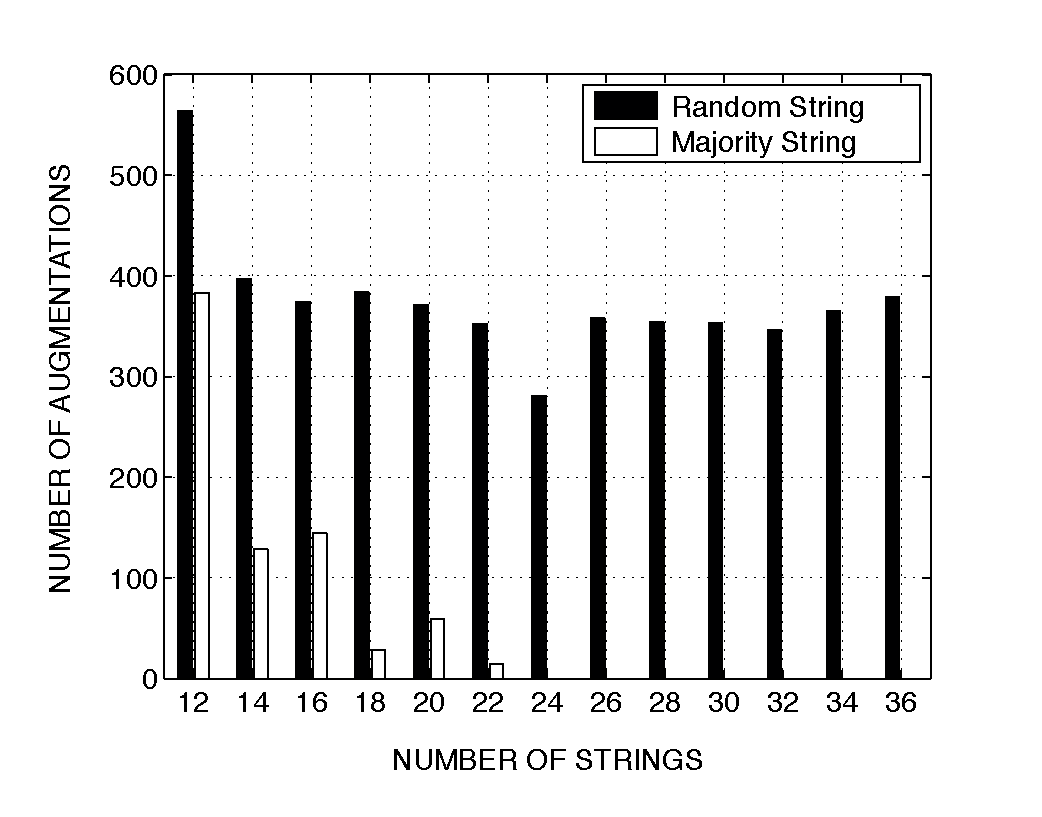
\includegraphics[width=\linewidth]{images/maj_vs_rand}% picture filename
 \caption[A comparison between the number of augmentations required to obtain a center string when procedure {\em augment} begins with a random string, and that required when procedure {\em augment} begins with a majority string, for various values of $n$.]{A comparison between the number of augmentations required to obtain a center string when procedure {\em augment} begins with a random string (shown in black), and that required when procedure {\em augment} begins with a majority string (shown in white), for various values of $n$. In all experiments, we have $\ell$ and $d$ equal to 15 and 4, respectively.}
\label{maj_vs_rand_fig}
\end{figure}

Figure \ref{maj_vs_rand_fig} demonstrates that the number of augmentations required to obtain a center string is significantly larger if $s_{maj, 0}$ is initialized to be a random string, rather than a majority string. Further, as the value of $n$ increases the disparity between the number of required number of augmentations of a majority string to obtain a center string and the required number of augmentations of a random string to obtain a center string increases substantially.  In particular, when $n$ is equal to 24 the number of augmentations required of the majority string is equal to 0 (as seen in Figure \ref{maj_vs_rand_fig}) -- illustrating that the majority string is a center string for all motif sets considered.  We observe that this fact cannot be extended to be true for random strings.
 
\begin{figure}[h!]
\centering
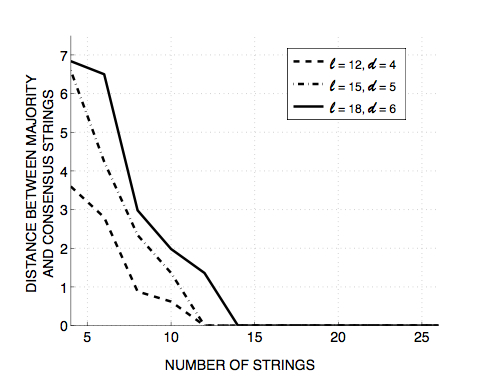
\includegraphics[width=\linewidth]{images/graph2v2}% picture filename
 \caption[An illustration of the decrease in the mean distance between a majority and center string as $n$ increase, for various values of $\ell$ and $d$.]{An illustration of the decrease in the mean distance between a majority and center string as $n$ increase, for various values of $\ell$ and $d$. Each line represents the mean Hamming distance for differing values of $n$. }
\label{fig2}
\end{figure}
 
Next, we considered the change in the Hamming distance as the values $n$, $\ell$, and $d$ varied.  We considered three different value of $\ell$ and $d$, varied the value of $n$ from 5 to 25, generated 100 random motif instances, and determined the mean Hamming distance between a majority string and a center string.  Figure \ref{fig2} illustrates this data and demonstrates a drastic decrease in the Hamming distance between the majority string and the center string as $n$ increases, for all the $(\ell, d)$-motif problems considered.  When the value of $n$ is significantly large, the distance between the majority string and the center string is equal to zero -- implying the majority string is a center string. 

Hence, the experimental results in this subsection illustrate the following trend: regardless of the value of $\ell$ and $d$ considered, for significantly large values of $n$ the majority string is likely to be a center string. 

\subsection{Empirical Evaluation of CSP-Greedy} 

{\em CSP-Greedy} begins with a string chosen at random from all majority strings, $s_{maj, 0}$, and iteratively augments $s_{maj, 0}$ so each time it is closer to at least one of the strings in $S$.  We consider how the number of augmentations of $s_{maj, 0}$ required to obtain a center string is affected if $s_{maj, 0}$ is initialized to a majority string, rather than a random string. 


 
\begin{table*}[h!]
\begin{center} {
	\begin{tabular}{|c|c|c||c|c|c| }
     \hline	
	$n$				& Mean accuracy 			& Mean number of		 & $n$ 			& Mean accuracy			&	Mean number of  \\
						&  						& augmentations	 & 	 			& 							& augmentations \\
	\hline
    4						& 57 			& 416 	& 16				&	99 				&	256			\\
	6  					& 86 			& 540 	& 18				&	100 				& 0\\
	8		 				& 87 			& 832 	& 20				& 100 							& 0 \\
	10					& 92 			& 800 	& 22				& 	100								& 0 \\
	12					& 98 			& 288 	& 24				& 	100 								& 0 \\
	14					& 98 			& 392 	& 26				& 	100 								& 0 \\
	\hline
	\end{tabular}}
\end{center}
\caption[Data illustrating the change in the accuracy and efficiency of {\em CSP-Greedy} as the value of $n$ increases.]{Data illustrating the change in the accuracy and efficiency of {\em CSP-Greedy}  as the value of $n$ increases.  We varied the value of $n$, and fixed $\ell$ and $d$ to be 10 and 3, respectively. We generated 1000 motif sets for each value of $n$, determined the number of augmentations of procedure {\em augment} to obtain a center string from a majority string, and calculated the mean of these 1000 values.}
\label{table2}
\end{table*} 

\subsubsection{Number of Input Strings}

The number of strings has a substantial effect on the running time of {\em CSP-Greedy}. Table \ref{table2} outlines the relationship between the value of $n$ and the accuracy and efficiency of {\em CSP-Greedy}. The mean accuracy of the algorithm is the percentage of motif sets where {\em CSP-Greedy} finds a center string.  We varied the value of $n$, and fixed $\ell$ and $d$ to be 10 and 3, respectively. We generated 1000 motif sets for each value of $n$, determined the number of augmentations of procedure {\em augment} to obtain a center string from a majority string, and calculated the mean of these 1000 values.  For this set of experiments we increased the maximum of augmentations to 1000.  Table \ref{table2} shows that when $n$ becomes significantly large ({\em i.e.}\ $n$ is equal to 18) the majority string is a center string.  
 
 
Figure \ref{fig:csp_greedy_plot_v2} illustrates the change in the running time of algorithm as $n$ increases.  Even for significantly large value of $\ell$ and $d$ ({\em i.e.}\ when $\ell$ was equal to 29 and $d$ was equal to 10), the algorithm ran extremely efficiently.  For each set of values of $n$, $\ell$, and $d$, 1000 motif sets were generated, {\em CSP-Greedy} was ran on each set, and the mean running time was recorded.  The running time decreases significantly as $n$ increased for all values of $\ell$ and $d$ considered.  Out of all the motif sets we considered, a center string was not obtained for 21 of these sets.   

\begin{figure}[h!]
\centering
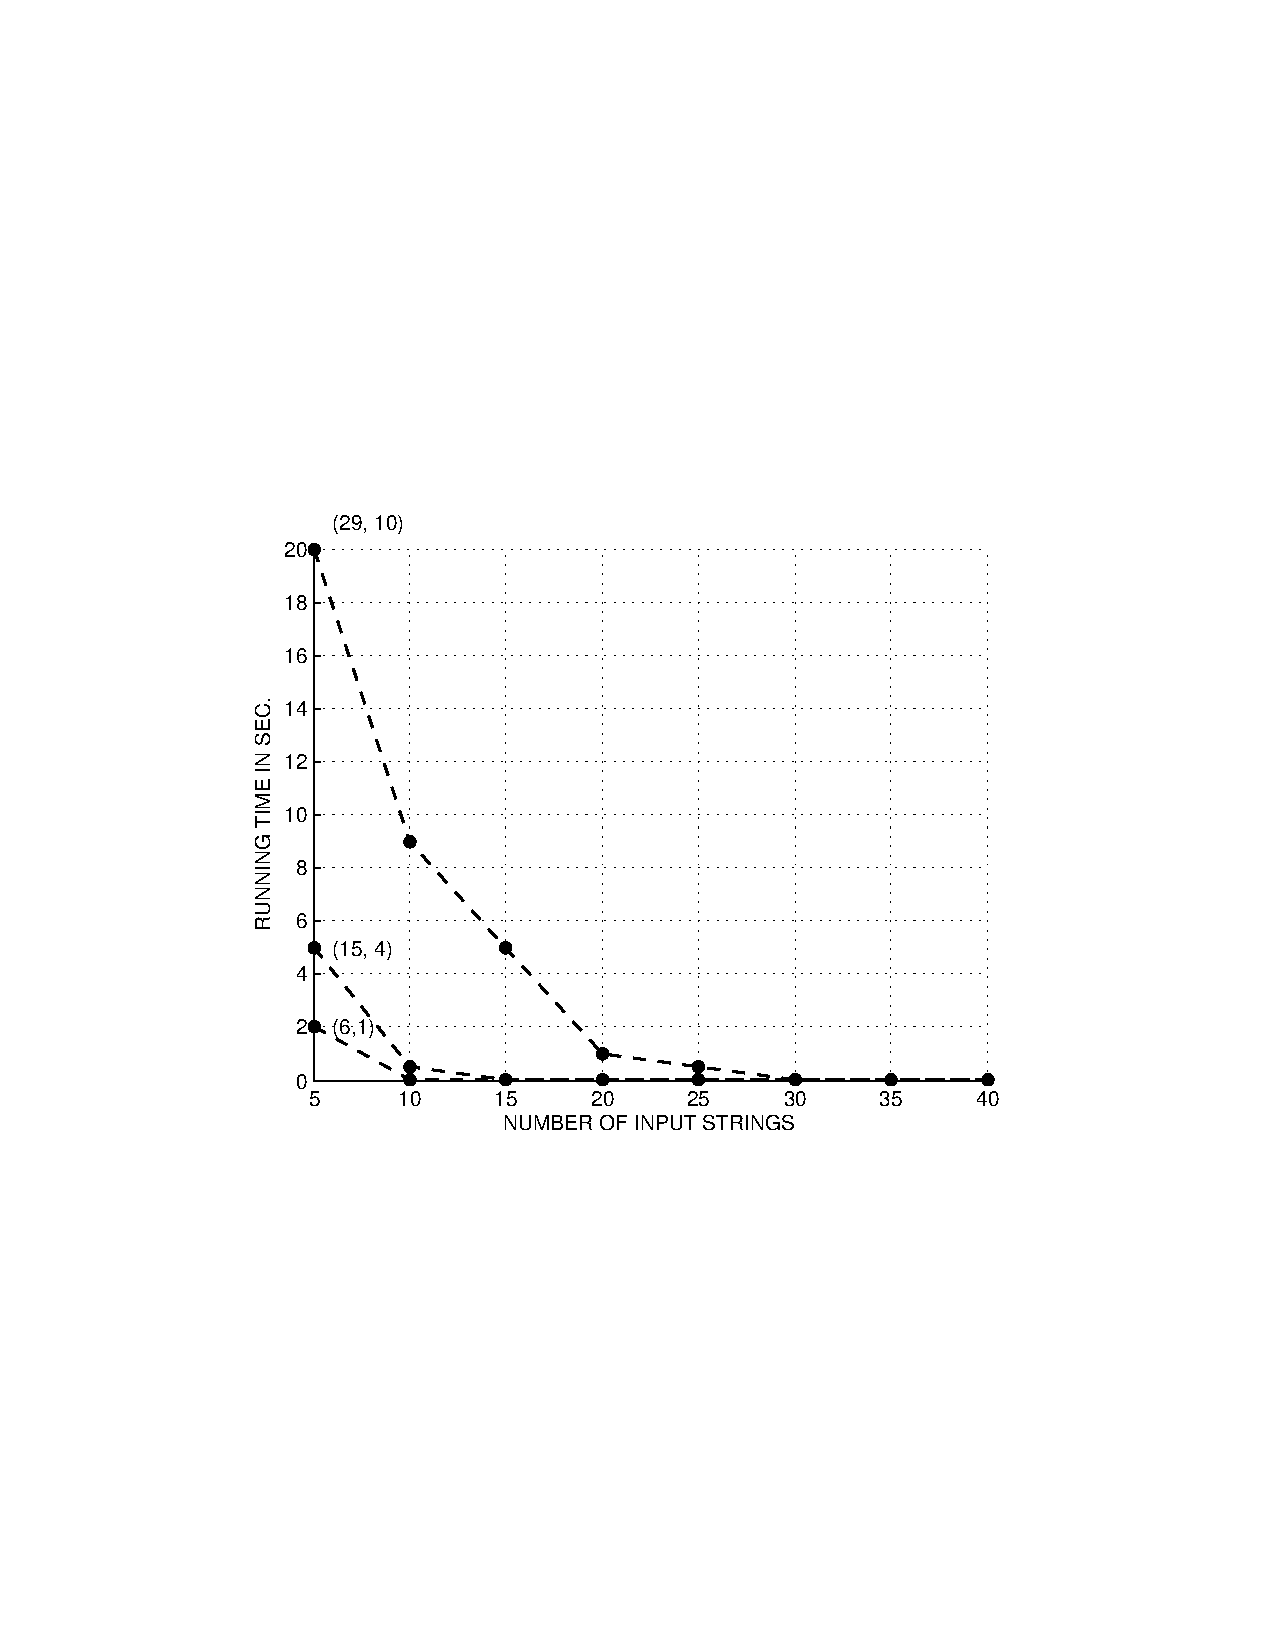
\includegraphics[width=65mm,trim=7cm 8cm 7cm 7cm]{images/csp_greedy_running_v2}% picture filename
 \caption[An illustration of the time required by {\em CSP-Greedy} to obtain a center string as $n$ increases, for various values of $\ell$ and $d$.]{An illustration of the time required by {\em CSP-Greedy} to obtain a center string as $n$ increases, for various values of $\ell$ and $d$.}
\label{fig:csp_greedy_plot_v2}
\end{figure}

\subsubsection{Length/Degeneracy Ratio}

We consider the change in the accuracy as $\ell$ and $d$ increase.  Again, we generated 1000 random motif sets, and obtained the mean accuracy and number of augmentations from running Procedure {\em augment} (with the number of augmentations increased to 1000).  Table \ref{closest_string_chapter:table1} illustrates the data from these experiments and shows that when $n = 20$ the mean number of augmentations was equal to zero for majority of values of $\ell$ and $d$, implying that the majority string was a center string.

\begin{table*}[h!]
\begin{center}{ 
\begin{tabular}{|cc||c|c|}
\hline
 		&  			& \multicolumn{2}{c|}{$n = 5$} \\
\hline
$\ell$ 		& $d$ 		& Mean accuracy 		& Mean number of augmentations\\
\hline
\hline
   6			& 1			& 97 			& 270 			 \\
	8  		& 2			& 83 			& 272	 		\\
	10		& 3 			& 67 			& 825 			\\
	12		& 3			& 86 			& 504 			\\	
	14		& 4			& 63 			& 813 		 \\
	15		& 4			& 69 			& 744 		 \\
	18		&	6			& 61 			& 920 		 \\
	21		& 7			& 62 			& 912 		 \\
\hline
		&			& \multicolumn{2}{c|}{$n = 15$}  \\
\hline
   6			& 1			& 100 			& 0				 \\
	8  		& 2			& 100 			& 0 				 \\
	10		& 3 			& 99			& 225	 				\\
	12		& 3			& 100 			& 0 				 \\	
	14		& 4			& 99 			& 440	 		\\
	15		& 4			& 99  			& 506	 \\
	18		&	6			& 96 			& 916	 \\			
	21		& 7			& 93 			& 945	 \\
\hline
&& \multicolumn{2}{c|}{$n = 20$} \\
\hline
   6			& 1				& 100  		& 0 \\
	8  		& 2				& 100  		& 0 \\
	10		& 3 			& 100  		& 0	\\
	12		& 3				& 100  		& 0 \\	
	14		& 4		& 100  		& 0 \\
	15		& 4			& 100  		& 0 \\
	18		&	6							& 96 		& 183 \\
	21		& 7				& 97  		& 291 \\
\hline
\end{tabular} }
\end{center}
\caption[Data illustrating the change in the accuracy and efficiency of {\em CSP-Greedy} as $\ell$ and $d$ increase.]{Data illustrating the change in the accuracy and efficiency of {\em CSP-Greedy} as $\ell$ and $d$ increase.The mean accuracy and number of augmentations represents the results obtained for 1000 randomly generated motif sets.}
\label{closest_string_chapter:table1}
\end{table*} 
\newpage

Figure \ref{fig:csp_greedy_plot} illustrates the change in the running time of {\em CSP-Greedy} as $\ell$ and $d$ vary, and $n$ is fixed at 20.  When the $\ell / d$ ratio became significantly large the running time was infinitesimal.  Again, for each set of values of $n$, $\ell$, and $d$, 1000 motif sets were generated, {\em CSP-Greedy} was run on each set, and the mean running time was recorded.  Out of the 24,000 sets considered, a center string was not obtained for 42 of the sets.   

\begin{figure}[h!]
\centering
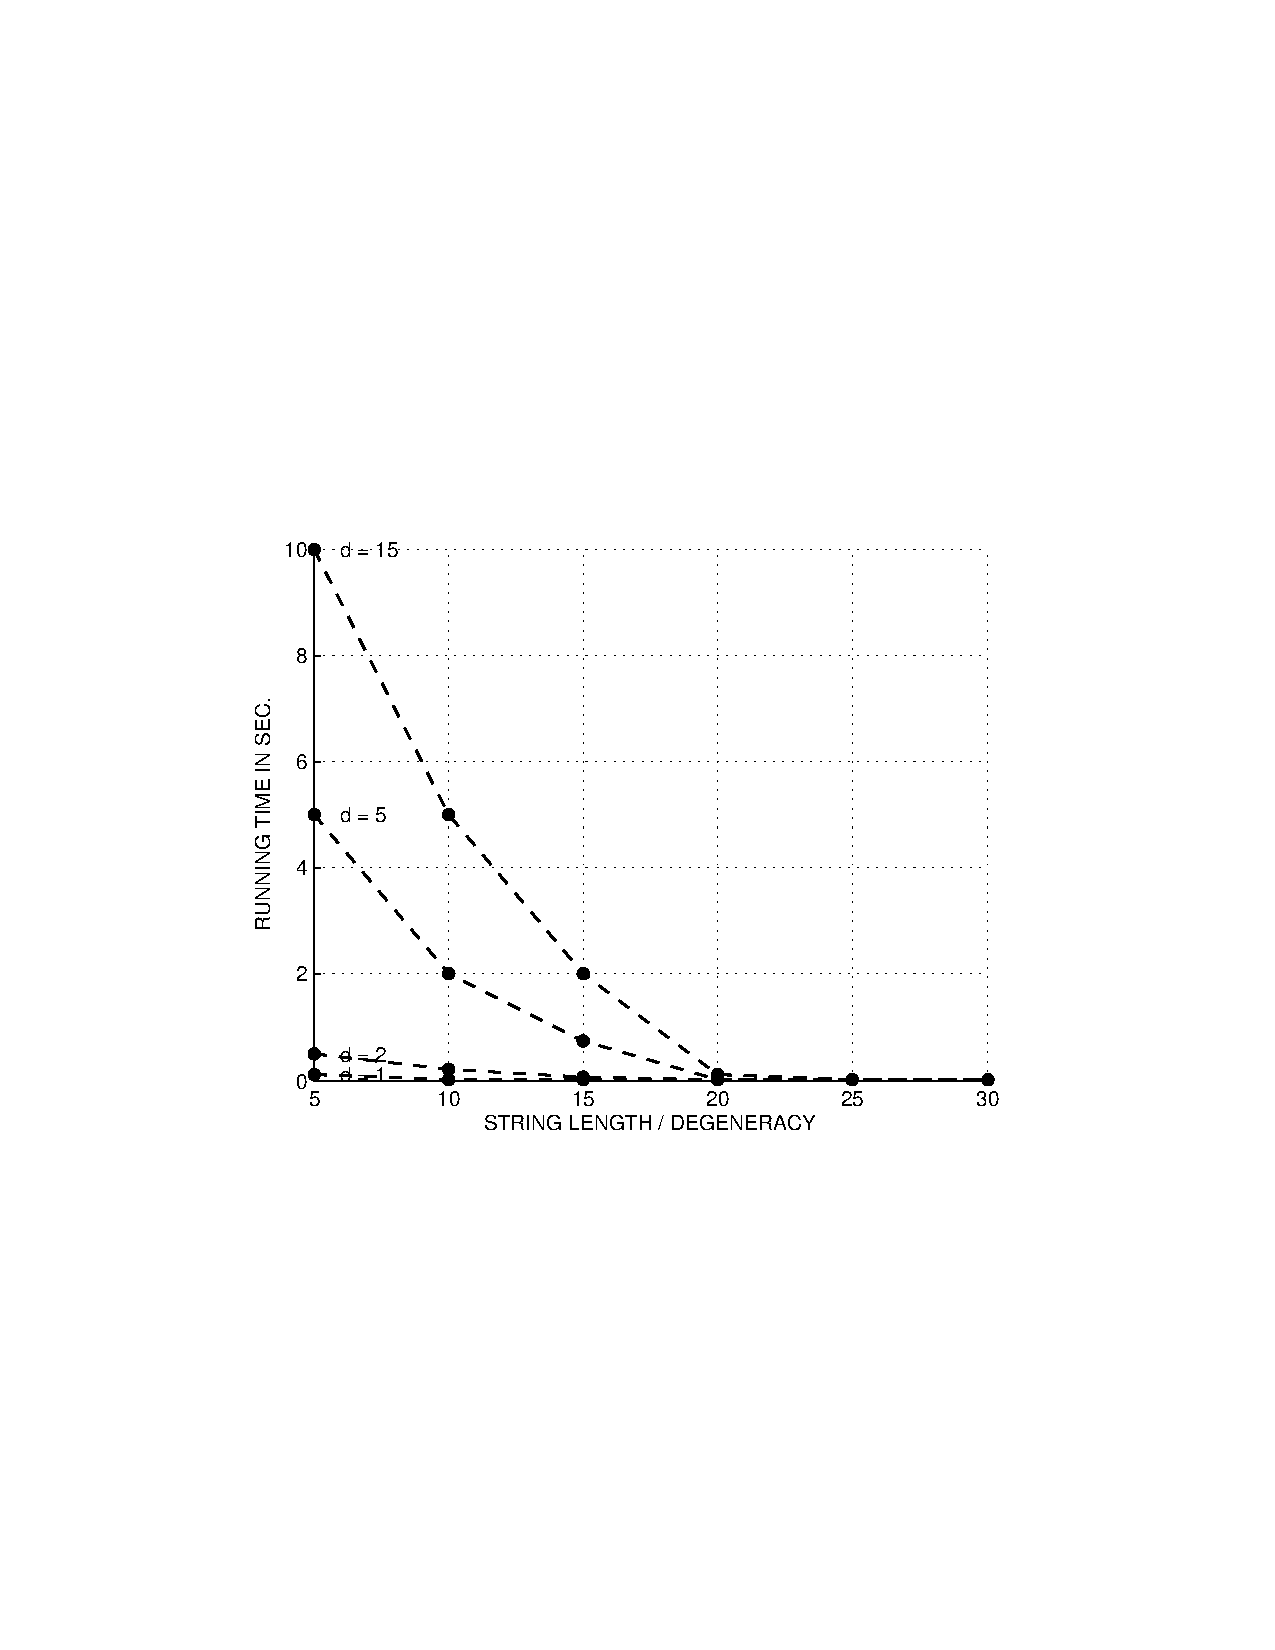
\includegraphics[width=65mm,trim=7cm 8cm 7cm 7cm]{images/csp_greedy_running_time_v1}% picture filename
 \caption[An illustration of the time required by {\em CSP-Greedy} to obtain a center string as $\ell/d$ ratio increases, for various values of $d$.]{An illustration of the time required by {\em CSP-Greedy} to obtain a center string as $\ell/d$ ratio increases, for various values of $d$. In these experiments, $n$ is equal to 20. }
\label{fig:csp_greedy_plot}
\end{figure}


\subsection{Application to Motif Recognition} 

MCL-WMR was developed specifically for the problem of detecting weak motifs in genetic data and works by first building a weighted graph model of the given motif-recognition problem and then using a graph clustering algorithm to quickly determine important subgraphs that need to be searched further for valid motifs. These smaller subproblems are then solved optimality using a dynamic-programming algorithm for finding motifs in dense subgraphs.  We extend MCL-WMR to incorporate {\em CSP-Greedy}. This new algorithm, {\em pMCL-WMR}, detects motifs in data sets with a large number of strings.  More specifically, pMCL-WMR efficiently discovers motifs in data sets that have 30 or more strings, and finds regulatory strings in genomic data.  

\subsection{Performance of pMCL-WMR on Synthetic Data}

We produced problem instances as follows: we chose a random center string of length $\ell$, and picked $m$ occurrences of the motif by randomly choosing $d$ positions per occurrence and randomly mutating the base at each. We constructed $m$ background strings of length $n$ and inserted the generated motifs into a random position in the string.  For each of the $(\ell, d)$ combinations, 100 random sets of input strings ($n = 20$, $m = 1000$) were generated. The running time is given in CPU seconds.  

Table \ref{table3} shows the comparison between the running time of MCL-WMR and that of pMCL-WMR. Two significant trends are witnessed in the data: pMCL-WMR is capable of solving hard instances of motif recognition ({\em i.e.}\ when $\ell = 25$ and $d = 7$) and pMCL-WMR gives a dramatic improvement over MCL-WMR with respect to the running time for all values of $\ell$ and $d$. The main advantage to our tool is the time required to solve the extremely difficult challenge problems -- from the $(18, 6)$ to the $(25, 7)$ problem -- in substantially better running time and with 100\% accuracy. 

The computational results in Subsection \ref{sec:cspgreedy_vs_fpt} inspire the investigation of instances with a significantly large number of sequences -- that is, instances where $n$ varies from values greater than 20. Table \ref{table4} shows the evaluation of the performance of pMCL-WMR on a range of problems with an increasing number of sequences.  The efficiency on these sets of problems is noteworthy ranging from 781 (when $n = 18$) to 2781 ($n = 30$). As far as we are aware, these are the first computational experiments where $n$ is larger than 20. 

An entry ``-'' indicates that the program was unable to solve the specific problem in a reasonable amount of time. The mean running time is given, followed by the standard deviation. 

\begin{table*}[h]
\begin{center} {
	\begin{tabular}{|c|c|c|}
     \hline	
	$(\ell, d)$	 		& MCL-WMR		& pMCL-WMR	 \\
	\hline
    (10, 2)				& 1003 / 32 		& 518 / 11			\\
    (15, 4)				& 3232 / 92			& 788 / 22			\\
	(16, 5)  			& 4200 / 103		& 1529 / 31				\\
	(18, 6)		 		& 8905 / 150		& 1723 / 47 			\\
	(25, 7)				& -						& 	2923 / 45		\\
	\hline
	\end{tabular}} 
	\end{center}
\caption[Comparison between the performance of MCL-WMR and that of pMCL-WMR on synthetic data. ]{Comparison between the performance of MCL-WMR and that of pMCL-WMR on synthetic data. In all experiments, $m = 1000$, $n = 20$, and $\ell$ and $d$ are varied. The mean and standard deviation of the running time in CPU seconds is given. }
\label{table3}
\end{table*}


\begin{table*}[h]
\begin{center} {
  \begin{tabular}{|c|c|c|c|}
     \hline	
	$n$				& MCL-WMR 	& pMCL-WMR	 \\
	\hline
    18				& 1981 / 65		& 781 / 23 \\
	20  				& 3233 / 82  	& 931 / 45 \\
	24		  	  	&	-					& 1721	/ 72	\\
	28				&  - 					& 1200	/ 87 \\
	30				&  - 					& 2781	/ 91		 \\
	\hline
	\end{tabular}}
\end{center}
	\caption[Comparison between the performance of MCL-WMR and that of pMCL-WMR on synthetic data as $n$ increases.]{Comparison between the performance of MCL-WMR and that of pMCL-WMR on synthetic data as $n$ increases. In all experiments, $\ell = 15$, $d = 4$ and $m = 1000$. The mean and standard deviation of the running time in CPU seconds is given. } 
	\label{table4}
\end{table*}
 	
\subsection{Using pMCL-WMR to Find Regulatory Elements}

An important biological challenge is to determine regulatory elements in DNA -- specifically, binding sites for transcription factors.  In this section, we demonstrate the use of pMCL-WMR in discovering these DNA sequence ``motifs'' in data sets with a large number of DNA sequences. Tompa {\em et al.}\ \cite{tompa} extensively assess 13 motif-recognition tools using test sets that make use of transcription factor binding sites. The binding sites were obtained from the TRANSFAC database \cite{WDKK96} and contain eukaryotic transcription factors.  The TRANSFAC database is extremely comprehensive, containing data from a large variety of species ({\em i.e.}\ species include yeast, {\em mus}, {\em oryctolagus cuniculus}, and {\em homo sapiens}) \cite{WDKK96}. For more details concerning the data set, including the selection process for transcription factors and binding sites from TRANSFAC, see Tompa {\em et al.}\ \cite{tompa}.  

Each transcription factor gives rise to one set of sequences. The number of sequences varied from 34 to 6 and the sequence length (parameter $m$) varied from 700bp to 2000bp. The transcription factor binding sites vary in length and thus, in order to assess pMCL-WMR, we ran the program on varied values $\ell$ and $d$.  The lengths of the motifs were same as those of the published motifs and $d$ varied.  Experimental results are shown in Table \ref{bio_table}.  pMCL-WMR was capable of discovered all of the motifs sets reported by Tompa {\em et. al.}\ \cite{tompa}, as well as some undetected motifs.  The motifs discovered only by pMCL-WMR and not by  any of the motif-recognition programs assessed by Tompa {\em et. al.}\ \cite{tompa} are shown in Table \ref{bio_table}. 

\begin{table*}[h]
\begin{center} {
	\begin{tabular}{|c|c|c|c|}
     \hline	
	Data set 	& $(\ell, d)$ & $n$ & Motif pattern discovered  \\
	\hline
	hm06		& (7, 1) &	9	 & TttTccC		   \\
	hm06		& (8, 1) & 9 & GGAcTGCT		    \\
	hm10		& (8, 3) & 6 & TTTcgCGC		  \\	
	hm13		& (10, 2) & 6 & aaAATTatTC		   \\
	hm13		& (11, 1) & 6	 & tccCcCACAaa		    \\
	hm19		& (11, 2) & 5 & tccCcCACAaa		    \\ % check this
	\hline			
   	\end{tabular}}
\end{center}
\caption[Illustration of the regulatory strings found by pMCL-WMR]{Illustration of the regulatory strings found by pMCL-WMR. Data are collected from SCPD.  For each set of data, we determined motifs of the same length using pMCL-WMR, and gave the motif published by Tompa {\em et. al.} \cite{tompa} for the same data set.  }
\label{bio_table}
\end{table*}


\begin{table*}[h]
\begin{center} {
	\begin{tabular}{|c|c|c|c|}
     \hline	
	Data set	& $(\ell, d)$ & $n$& Time \\
	\hline
	hm06		& (7, 1) &	9		& 80 \\
	hm06		& (8, 1) & 9		& 102 \\
	hm10		& (8, 3) & 6		& 210\\	
	hm13		& (10, 2) & 6		& 178 \\
	hm13		& (11, 1) & 6		& 220 \\
	hm19		& (11, 2) & 5		& 321\\ % check this
	\hline			
   	\end{tabular}}
\end{center}
\caption[CPU time required by pMCL-WMR to detect the regulatory sequence patterns shown in Table \ref{bio_table}]{CPU time required by pMCL-WMR to detect the regulatory sequence patterns shown in Table \ref{bio_table}.}
\label{bio_table:runtime}
\end{table*}

\section{Summary and Open Problems}

In this chapter, we gave a linear-time algorithm for solving {\sc Closest String} problem with four binary strings, proved lower and upper bounds for the approximation guarantees for a simple probabilistic algorithm for the general problem, and showed the existence of an algorithm with running time $O(\ell^3)$ that achieves a $\left(1  - \left( \frac{\epsilon}{ 2^{n}} \right)^{\ell}\right)$-approximation, for some small $\epsilon > 0$ and significantly large values of $n$.  Our smoothed analysis of {\em CSP-Greedy} gives reasons as to why this algorithm and the $O(n\ell + nd \cdot d^d)$-time algorithm of Gramm {\em et al.}\ \cite{GNR03} is efficient in practice for {\sc Closest String} instances with a large number of strings. This analysis gives an analytical reason to why this -- and perhaps other similar {\sc Closest String} algorithms -- perform well in practice.  Lastly, we gave empirical results that demonstrate the majority string is likely to be a center string when the number of sequences is moderately large.  

There exist numerous open problems that warrant further investigation, including the following:

\begin{itemize}
\item Since the publication of the linear-time algorithm presented in this chapter, these results have been extended by Amir {\em et al.}\ \cite{amir} to a variant of the {\sc Closest String} problem. Determining how these results could be generalized to larger alphabets or to instances containing more than four strings remains open. Such a generalization would invite many open problems in motif recognition to be revisited, as their tractability might be determined more concretely. 

\item In smoothed analysis one often analyzes how fragile worst case instances are. Manthey and Reischuk \cite{MR05} suggest examining the dual property of how robust the best (or good) instances are.  Lastly, we propose continuing this form of analysis and determining how stable the best-case instances of the closest string problem are under perturbations. This would involve considering instances where {\em CSP-Greedy} performs efficiently and showing that even large perturbations of these instances yield problems that can be solved in efficient time.

\item There exist several open problems related to the smoothed complexity of string selection problems that warrant investigation.  Analyzing the smoothed complexity of the PTAS of Li {\em et al.}\ \cite{LMW02} for the {\sc Closest String} problem requires further study.  The running time of this PTAS is detrimentally large, thus reducing the algorithm to only theoretical importance.  However, there have been several papers attempting to prove that the algorithm performs significantly better in practice \cite{brona1,brona2}; the smoothed analysis of the algorithm would potentially complete this area of study.
\end{itemize}
%======================================================================
\chapter{{\sc Closest String with Outliers}}\label{chapter:cswo}
%======================================================================

Finding similar regions in multiple DNA, RNA, or protein sequences plays an important role in many applications, including universal PCR primer design \cite{DRSS,LLMWZ00,LBOT,PH}, genetic probe design \cite{LLMWZ00}, antisense drug design \cite{DLLM,LLMWZ00}, finding transcription-factor binding sites in genomic data \cite{tompa}, determining an unbiased consensus of a protein family \cite{BLPR}, and motif recognition \cite{LLMWZ00,Pav01,PS00}.  Up to this point, we have formulated these problems with respect to the {\sc Closest String} problem, which was first introduced and studied in the context bioinformatics by Lanctot {\em et al.}\ \cite{LLMWZ00}.  Since its introduction, the investigation of efficient polynomial time approximation algorithms and exact exponential time algorithms for the {\sc Closest String} problem has been thoroughly considered~\cite{FGN06,FGN,GNR03,LLMWZ00,LMW02,ma00,MS08}. However, in many contexts the {\sc Closest String} problem can be too restrictive.  In this chapter we consider the computational tractability and intractability of a less-restrictive version of this problem, and in the following one, we illustrate the applicability of this version.  

The {\sc Closest String} problem requires that the Hamming distance constraint be satisfied for each of the input strings and therefore, is robust to the overrepresentation of the input strings; regardless of the number of occurrences of a distinct string, the Hamming distance constract must be still satisfied.  For this reason it is frequently used to model many of the aforementioned applications.  However, this property also causes a severe problem: if the input includes a string that is significantly different from the other input strings, which we refer to as an ``outlier'', then it will have the effect that a centre string for the complete set of input strings will not exist; $d$ will have to be increased dramatically to account for this string and obtain a center string. This is a significant limitation for applications such as the design of universal primers where a small $d$ is crucial for the effectiveness of the primers.  In this and many other applications, it would be preferable to determine a ``good'' center string ({\em i.e.}\ one that is reasonably close to each of the strings) for a large portion of the input strings rather than trying to find a center string for the complete set and in doing so finding one that is a large distance from many or all of the strings.   Hence, we aim to model the task of finding a center string that is within (reasonably small) distance $d$ of most of the input strings, not necessarily all.  Another compelling consequence of the modification of the model is that in situations where a more satisfying solution can be found by regarding a few strings as outliers, the initial decision of including them requires re-examination.

We formally model this problem as follows:\\

\noindent{\sc Closest String with Outliers (CSWO) } \\
\noindent{\sc Input:} A set of $n$ length-$\ell$ strings $S = \{s_1, \ldots, s_n\}$ over a finite alphabet $\Sigma$ and nonnegative integers $k$ and $d$.\\
\noindent{\sc Question:} Find a center string $s$ and a subset of $S^* \subset S$, such that $|S^*| = n-k$ and $d(s,t)\le d$ for $t\in S^*$.\\

We denote $n - k$ as $n^*$, and the symbol at position $p$ of string $s_i$ to be $s_i(p)$.

There exists a simple reduction from the {\sc Closest String} problem to {\sc CSWO} that demonstrates it is NP-complete even in the special case where the alphabet is binary and $k=0$, implying it is unlikely to be solved exactly by a polynomial-time algorithm, unless P=NP.  One approach to investigating the computational intractability of {\sc CSWO} is to consider its parameterized complexity, which aims to classify computationally hard problems according to their inherent difficulty with respect to multiple parameters of the input. If it is solvable by an algorithm that is polynomial in the input size and exponential in parameters that are typically small then it can still be considered tractable in some practical sense.

Smith \cite{asmith} introduced a related optimization problem.  Given a set $S = \{S_1, \ldots, S_n\}$ of $m$-length sequences over the alphabet $\Sigma$ and integers $d$ and $\ell$, the aim of the {\sc Maximum Coverage Approximate Substring} problem is to maximize $|S'|$, $S' \subseteq S$, such that for some $s \in \Sigma^{\ell}$ and for all $S_i \in S$, where there exists a substring $s_i \in S_i$ such that $d(s, s_i) \leq d$.  Smith demonstrated that this problem is APX-hard, and gives a $|\Sigma|^d$-approximation algorithm for this problem.  
  
For unbounded alphabet size, we show that {\sc CSWO} is W[1]-hard for every combination of the parameters $\ell$, $d$, and $n^*$ and thus, is fixed parameter intractable when parameterized by any subset of these parameters, unless FPT = W[1].  We also show that when the alphabet is unbounded, there exists a fixed-parameter tractable algorithm for {\sc CSWO} with respect to the parameters $d$ and $k$.  In the case of a constant-size alphabet {\sc CSWO} is fixed parameter tractable for the parameter $n$ but intractable for the parameter $k$.  The complexity of the problem remains open when parameterized by $d$ and the alphabet is of constant size, and when parameterized by $n^*$ and $k$.  

\section{{\sc Closest String with Outliers}: Tractability \\ Results}

We first consider $\Sigma$ as a parameter.  In computational biology applications the biological sequences of interest are typically DNA or protein sequences and hence the number of different symbols is a small constant ({\em i.e.}\ 4 or 20 in the case of DNA or protein sequences, respectively).  Restricting $\Sigma$ only does not make {\sc CSWO} tractable since it is NP-hard even when the alphabet is binary. However, if $\Sigma$ and $\ell$ are both parameters then it is fixed-parameter tractable; we can enumerate and check all the $|\Sigma|^{\ell}$ possible center strings.  We show in this section that the problem is fixed parameter tractable with respect to the parameters $\Sigma$, $\ell$, $d$ and $n$.  We will prove in a later section that it is imperative that $\Sigma$ be a parameter in order to obtain this tractability. 

\begin{algorithm*}[h]
\caption{CSWO Algorithm}
\begin{algorithmic}
\STATE {\bf Input: } A {\sc CSWO} instance with a set of $S$ $n$ strings of length $\ell$, parameters $\Delta d$, $d$ and $k$, and a candidate string $x$.
\STATE {\bf Output:} A string $s^*$ if there exists a set $S$ of at least $n^*$ strings where each string in $S$ has distance at most $d$ from $s^*$, and ``Not found'' otherwise.
\STATE
\STATE If $\Delta d < 0$ or $k < 0$ then return ``Not found''
\STATE Choose $i \in \{1, \ldots, n\}$ such that $d(x, s_i) > d$. If no such $i$ exists return $x$.
\STATE $s_{ret}$ =  {\sc CSWO} Algorithm ($S \, \backslash \, \{ s_i \}$, $\Delta d$, $k - 1$, $x$)
\STATE If $s_{ret}$ = ``not found '' then
\STATE \hspace{5mm} $\mathcal{P} = \{p \, |  \, x(p) \ne s_i(p)\}$;
\STATE \hspace{5mm} Choose any $\mathcal{P}'$ from $\mathcal{P}$ with $|\mathcal{P}'| = d + 1$.
\STATE \hspace{5mm} For each position $p \in \mathcal{P}'$
\STATE \hspace{10mm} Let $x$ be equal to $s_i$ at position $p$ 
\STATE \hspace{10mm} $s_{ret}$ = {\sc CSWO} Algorithm ($S$, $\Delta d - 1$, $k$, $x$) 
\STATE \hspace{10mm} If $s_{ret} \neq $ ``not found '', then return $s_{ret}$
\STATE Return ``not found''
\end{algorithmic}
\end{algorithm*}

The fixed parameter algorithm that we present is very similar to the algorithm presented by Gramm {\em et al.}\ \cite{GNR03}, where it is proved that {\sc Closest String} is fixed parameter tractable with respect to the parameter $d$. In the algorithm by Gramm {\em et al.}\ \cite{GNR03} at each recursive step a string $s$ is selected that has Hamming distance at least $d+1$ away from the current candidate center string $x$ if one exists; otherwise $x$ is returned since it is a center string.  Then for any $d+1$ positions where $x$ and $s$ disagree, there is at least one position at which $s$ is equal to the final solution.  The algorithm tries each of the $d+1$ positions, changes $x$ to $s$ at one of the $d+1$ positions, reduces $\Delta d$ by one, and calls itself recursively.  Since the recursion stops after at most $d$ steps, the size of the search tree is bounded by $O((d + 1)^d)$.

Our algorithm begins with $s_1$ as the candidate center string.  If $s_1$ is a center string with respect to $S$ then we are done; otherwise there exists a string $s_i$ that has distance at least $d + 1$ from $s_1$.  We determine whether $s_i$ belongs in the set of outliers by trying both possibilities: $s_i$ belonging in the set of outliers and $s_i$ not belonging in the set of outliers.  If it is an outlier then we remove it from $S$ and recurs on the smaller set with $k - 1$.  If it is not an outlier then we use $s_i$ to move the candidate string $x$ closer to toward $s_i$, which can be done by applying the methodology of Gramm {\em et al.}\ \cite{GNR03}. This will increase the size of the search tree.

\begin{proposition} The {\em CSWO Algorithm} solves the {\sc CSWO} problem in time $O(n \ell + n d \cdot d^d \cdot 2^{k+d})$. \end{proposition}

\begin{proof}  We first consider the running time of the algorithm and then subsequently, give proof of the algorithm's correctness.

{\bf Running time.} Each recursion of the algorithm reduces either $k$ or $d$ by 1.  Thus, there are at most $k+d$ guesses of whether a particular string belongs in the set of outliers. Thus, the search tree size is increased by a multiplicative factor of at most $2^{k+d}$ and the search tree size is bounded above by $O(2^{k+d} \cdot (d+1)^d)$.  The analysis of Gramm {\em et al.}\ \cite{GNR03} demonstrated that each recursive step takes time $O(nd)$ and the preprocessing time takes $O(n\ell)$ and therefore, we obtain an overall running time of $O(n \ell + n d \cdot d^d \cdot 2^{k+d})$.

{\bf Correctness} We show the correctness of our algorithm by showing the correctness of the first recursive step and then the correctness of the algorithm follows by inductively applying the following argument.  Clearly, if $S$ does not contain a subset $S^*$ of $n^*$ strings, such that there exists a center string $s^*$ for $S^*$ then ``not found'' will be returned and therefore, we assume otherwise.  

If $s_1$ is a center string for $S$ then the algorithm immediately halts so we assume there exists a string $s_i$ in $S$ that does not have $s_1$ as a center string.  When considering $s_i$, there are two subcases: one where $s_i$ is in the set of outliers, and another where $s_i$ is not.  Suppose $s_i$ is in the set of outliers; then the first case will successfully remove $s_i$ from the set and recurse on $S \, \backslash \, \{s_i \}$.  Otherwise, if $s_i$ is not in the set of outliers, then eventually the second case will be reached. We refer to the set of positions as {\em correct} if $\{ p \, | \, s_1(p) \ne s^*(p) = s(p)\}$.  It follows from Gramm {\em et al.}\ \cite{GNR03} that one of the $d + 1$ chosen positions $p$ will be a correct one. Thus, we have shown that either one of the subcases will lead to a smaller subcase containing the solution for $S$.  \hfill $\Box$ \end{proof} 

The previous result demonstrates the fixed-parameter tractability with respect to $d$ and $k$. We note that a similar modification of the $O(n |\Sigma|^{O(d)})$ algorithm of Ma and Sun \cite{MS08} also gives a fixed parameter algorithm with respect to the parameters $\Sigma$, $d$ and $k$.  In the modified algorithm, for any string $s$ with distance greater than $d$ to the current candidate center string $x$, we again try the subcases where $s$ is an outlier, and is not an outlier.  In the former case, we remove $s$ from the set of input strings $S$ and recurs on $S$ and $k  - 1 $, and in the latter case, we use the same technique as in the algorithm of Ma and Sun \cite{MS08} to reduce the distance between $x$ and the final solution.  This modification that accounts for the outliers results an extra multiplicative factor of $O(2^{k +\log d})$ to the running time of the original algorithm.  Although this algorithm improves upon the running time of the previous result, it requires that $\Sigma$ is also a parameter.  Further, we note that some of the recent improvements \cite{CMW,WZ,ZZ} to the algorithm of Ma and Sun can be modified in a similar manner to obtain fixed parameter algorithms for CSWO with respect to parameters $\Sigma$, $d$ and $k$.

\begin{proposition} \label{prop:fpt} {\sc CSWO} is fixed parameter tractable for parameters $\Sigma$ and $n$. \end{proposition}

\begin{proof} Gramm {\em et al.}\ \cite{GNR03} gave a fixed-parameter tractable algorithm for {\sc Closest String} with respect to the number of strings and $\Sigma$, which we refer to this algorithm as {\em ILP-procedure(S)}, where $S$ is the set of input strings.  Our algorithm enumerates all size-$n^*$ subsets of $S$, and calls {\em ILP-procedure} on each subset.  \hfill $\Box$ \end{proof}

The algorithm proposed in the proof of Proposition \ref{prop:fpt} has $O\left( (n \cdot f(\ell, n, d))^n \right)$ running time, where $f(\ell, n, d)$ is the time required for the fixed parameter tractable algorithm.   The algorithm of Gramm {\em et al.}\ \cite{GNR03} models the problem as an integer linear program with $n^{n + 1}$ variables and constraints and then applies the famous result by Lenstra \cite{Len}, which states that an integer linear program can be solved in polynomial time with a constant number of variables.   Specially, the result is as follows:

\begin{theorem} \cite{Len} The integer programming feasibility problem can be solved in $O(p^{9p/2} \cdot L)$ time, where $p$ is the number of variables and $L$ is the number of bits in the input.  \end{theorem}

\noindent Proposition \ref{prop:fpt}, as well as the original result of Gramm {\em et al.}\ \cite{GNR03}, is only or theoretical use since the combinatorial explosition in $n$ in the running time of the corresponding algorithms is huge, thus rendering these algorithms impractical.

%%%%%%%%%%%%%%%%%%%%%%%%%%%%%%%%%%%%%%%%%%%%%%%%%%%%%%%%

\section{{\sc Closest String with Outliers}: Intractability \\ Results}

We derive the W[1]-hardness result by a series of intermediate steps, aiming at a reduction from {\sc Clique} to {\sc Closest String with Outliers}.  This shows that {\sc Closest String with Outliers} is W[1]-hard for the combination of $\ell$, $d$, and $n^*$, when the alphabet is unbounded.  

\subsection{Reduction from {\sc Clique}} \label{w1_construction}

As previously described, we let the {\sc Clique} instance be given by an undirected graph $G=(V, E)$ with a set $V=\{v_1, v_2, \ldots, v_n\}$ of $n$ vertices, a set $E$ of $m$ edges, and a positive integer $t$ denoting the size of the desired clique.  We describe how to generate a set $S$ of ${{t}\choose{2}} |E|$ strings such that $G$ has a clique of size $t$ if and only if there is a subset of $S$ of size ${{t}\choose{2}}$, denoted as $S^*$, where there exists a string $x$ such that $d(s_i, x) \leq d$ for all $s_i \in S^*$.  We let $\ell = t$ and $d = t - 2$.  We assume that $t > 2$ since $t \leq 1$ produces trivial cases.  
 
We begin by describing the alphabet.  We assume $|\Sigma|$ can be unbounded, however, for any given instance obtained by our reduction from {\sc Clique}, $|\Sigma|$ is finite.  We define $\Sigma$ to be equal to the union of the following sets of symbols:
\begin{enumerate}
\item $\{v_i | \mbox{  for all } i = 1, \ldots, |V|\}$.  There exists one symbol representing each vertex in $G$.
\item Let $m = |E|$ then $\{c_{i,j,m} | i = 1, \ldots, t; \, j = 1, \ldots, t\}$.  There exists an unique symbol for each of the ${t\choose 2} \cdot |E|$ strings produced for our reduction. 
\end{enumerate}
Hence, we have a total of $|V| + {t\choose 2} \cdot |E|$ symbols.
 
Next, we generate a set of ${{t}\choose{2}} |E|$ strings $S = \{s_{1,1,1},  \ldots, s_{1,1,|E|}, s_{1,2,1}, \ldots, $ $s_{1,2,|E|}, \ldots, s_{t -1,t, |E|}\}$. Every string has length $t$ and will encode one edge of the input graph. For string $s_{i,j,m}$ we encode edge $e_m=  (v_r, v_s)$, where $1 \leq r < s \leq |V|$, but by letting position $i$ equal to $v_r$ and position $j$ equal to $v_s$ and the remaining positions equal to $c_{i,j,m}$. Hence, a string is given by $$s_{i,j,m}\, := \, [ c_{i,j,m} ]^{i - 1} v_r [ c_{i,j,m} ]^{j - i - 1} v_s [ c_{i,j,m} ]^{m - j}.$$  Clearly, this reduction runs in time $O(|V| + {t \choose 2} \cdot |E|)$

To clarify our reduction, we give an example. Let $G = (V, E)$ be an undirected graph with $V = {v_1, v_2, v_3, v_4}$ and edges $E = \{(v_1, v_2), (v_1, v_3), (v_1, v_4), (v_2, v_3)\}$ and let our {\sc Clique} instance have $G$ and $t = 3$.  Figure \ref{fig:example} illustrates the reduction.  Using $G$, we exhibit the above construction of ${t \choose 2} \cdot |E| = 12$ strings, which we denote as $S$.  We claim that there exists a clique of size 3 if and only if there exists a string $s^*$ of length $\ell = t = 3$ and subset $S^*$ of $S$ of size $3$ where $d(s, s_i) \leq d$ for all $s_i \in S^*$.  In this example, the center string $s$ is equal to $v_1 v_2 v_3$ and each string in the set $\{v_1 v_2 c_{121},  v_1 c_{132} v_3, c_{234} v_2 v_3\}$ is such that each string in $S^*$ has Hamming distance at most 1 from $s$.  

\begin{figure}[h!]
\begin{center} 
 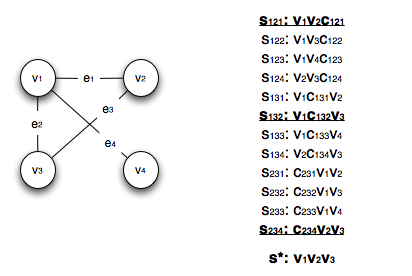
\includegraphics[width=\linewidth]{images/example}
\caption[An example showing the parameterized reduction from {\sc Clique} to {\sc CSWO}.]{An example of the parameterized reduction from a {\sc Clique} instance $G$ with $t = 3$ to an instance of {\sc CSWO} with 12 strings with $\ell = t = 3$, $d = t - 2 = 1$, and $n^* = {3 \choose 2} = 3$.  In bold we have the set of strings $S^* = \{s_{121}, s_{132}, s_{234}\}$ that corresponds to the clique containing the vertices $\{v_1, v_2, v_3\}$.  We note that $S^*$ is the only set of size 3 of strings with Hamming distance at most $d$ from the center string $s^*$. }
\label{fig:example}
\end{center}
\end{figure}

\subsection{Correctness of the Reduction}

The following two lemmas establish the correctness of the reduction. 

\begin{lemma} \label{direction_one_lemma} For a graph with a $t$-clique, the construction in Subsection \ref{w1_construction}  produces a {\sc CSWO} instance with a set $S^*$ and a string $s$ of length $\ell$ such that for every $s_i \in S^*$ $d(s_i, s) \leq d$. \end{lemma}

\begin{proof} Let the input graph have a clique of size $t$.  Let $v_{\alpha_1}, v_{\alpha_2}, \ldots, v_{\alpha_t}$ be the vertices in the clique $C$ of size $t$ and without loss of generality, assume $\alpha_1 < \alpha_2 < \ldots < \alpha_t$.  Then we claim that there exists a subset of ${t\choose 2}$ vertices that have distance at most $t - 2$ from the string $s = v_{\alpha_1} v_{\alpha_2} \ldots v_{\alpha_t}$.   Consider the first edge of the clique $(v_{\alpha_1}, v_{\alpha_2})$.  The string $s_{11r} = v_{\alpha_1} v_{\alpha_2} [c_{11r}]^{t - 2}$, where edge $r$ has endpoints  $v_{\alpha_1}$ $v_{\alpha_2}$, is contained in the set of strings $\{s_{111}, s_{112}, \ldots, s_{11|E|} \}$. Clearly, $H(s_{11r}, s) = t - 2$. For each edge in $C$ we have we have a string in $S$ that has distance at most $t - 2$ from $s$, as required.  \hfill $\Box$ \end{proof}

For the reverse direction, we need to prove that the existence of a subset $S^*$ of ${t \choose 2}$ and a string $s$ where $d(s, s_i) \leq t - 2$ for all $s_i \in S^*$ implies the existence of a clique in $G$ with $t$ vertices.  

\begin{lemma} \label{direction_two_lemma} If $(S, \ell, d, n, k)$ is a `YES' instance of the {\sc CSWO} problem then $(G, t)$ is a `YES' instance of the {\sc Clique} problem.  \end{lemma}

\begin{proof} Hence, we are required to show that the $t$ symbols of the center string correspond to the $t$ vertices of clique in the input graph.  Let $S^*$ be the subset of $S$ of size $t\choose 2$ such that $s$ has distance $t - 2$ from each string in $S^*$. Since $\ell = t$, $n^* = t$, $d = t -2$ and for each symbol $c_{i,j,m}$ there exists only a single string  $i = 1, \ldots, t$, $ j = 1, \ldots, t$ and $m = 1, \ldots, |E|$ it follows from the Pigeonhole principle that the center string $s$ only contains symbols from $\{v_i | \mbox{  for all } i = 1, \ldots, |V|\}$. Without loss of generality assume $s$ is equal to $v_{\alpha_1} v_{\alpha_2}\ldots v_{\alpha_t}$ for $\alpha_{v_1}, \alpha_{v_2}, \ldots, \alpha_{v_t} \in \{1, \ldots, |V|\}$. Consider any pair $\alpha_i, \alpha_j$ for $1 \leq i < j \leq t$ and consider the set of strings $S_{i,j} = \{ s_{i,j,1}, s_{i,j,2}, \ldots, s_{i,j,|E|} \}$.  Recall that $S_{i,j}$ contains a string corresponding to each edge $e = (r, s)$ in $E$ which has $v_r$ at the $i$th position and $v_s$ at the $j$th position and $c_{i,j,m}$ at all remaining positions.  Therefore, we can only find a string in $S_{i,j}$ that has distance at most $t - 2$ from $s$ if $v_{\alpha_i}$ is at the $i$th position and $v_{\alpha_j}$ is at the $j$th position; and such a string exists if and only if there is an edge in $G$ connecting $v_{\alpha_i}$ to $v_{\alpha_j}$. Hence, the center string $s$ implies there exists an edge between any pair of vertices in $G$ in the set $\{v_{\alpha_1} v_{\alpha_2}\ldots v_{\alpha_t}\}$ and by definition the vertices form a clique. \hfill $\Box$  \end{proof}

Our main theorem follows directly from Lemma \ref{direction_one_lemma} and Lemma \ref{direction_two_lemma}.  We note that the hardness for the combination of all three parameters also implies the hardness for each subset of the three. 

\begin{theorem} {\sc CSWO} with unbounded alphabet is W[1]-hard with respect to the parameters $\ell$, $d$, and $n^*$.\end{theorem}

Since there exists a trivial reduction from the {\sc Closest String} problem to {\sc CSWO} ({\em i.e.}\ simply set $k = 0$ in {\sc CSWO}), there cannot exist a fixed parameter tractable algorithm for {\sc CSWO} with $k$ as a parameter, unless P = NP; such an algorithm would contradict the NP-hardness of {\sc Closest String}. 

\begin{fact} {\sc CSWO} is W[1]-hard with respect to the parameter $k$, for any fixed $|\Sigma| \geq 2$. \end{fact}

%%%%%%%%%%%%%%%%%%%%%%%%%%%%%%%%%%%%%%%%%%%%%%%%%%%%%%%%%%%%%%%%%%%%%%%%%%%%%

\section{Summary and Open Problems}

We introduced the {\sc CSWO} problem, and proved that with unbounded alphabet size and parameterized by $\ell$, $d$ and $n^*$ it is W[1]-hard.  We also gave fixed parameter algorithms for the problem when parameterized by $d$ and $k$, and with unbounded alphabet size.  In the case of a fixed alphabet size, we showed {\sc CSWO} is fixed parameter tractable when parameterized by $n=n^*+k$. Table \ref{tab:results} summarizes these tractability and intractability results. Currently, the fixed parameter tractability of the {\sc CSWO} problem when parameterized by $d$, $n^*$ and $\Sigma$, and by $n^*$ and $k$, remains open (see Table \ref{tab:results}).  


\begin{table}
\begin{center}
\begin{tabular}{@{\hspace{0.5cm}}l  @{\hspace{0.5cm}}c @{\hspace{0.5cm}}c }
	\hline
  Parameter(s) 		 		& $|\Sigma|$ is a parameter  & $|\Sigma|$ is unbounded  \\
  \hline
  $\ell, d, n^*$ 			& FPT (trivial)							& W[1]-hard (*) \\  %% trivial
  $\ell$  						& FPT (trivial)							& W[1]-hard (*)\\ %% trivial
 % $d, n^*$ 					& FPT (*)									& W[1]-hard (*)\\ %% Follows from n^* being FPT
  %$n^*$ 						& Open									& W[1]-hard (*)	 \\ %% proof sketch  
  $d, n^*$ 					& Open										& W[1]-hard (*) \\
  $d, k$ 						& FPT (*)									& FPT (*) \\  %% proof sketch  
  $n^*, k$ 					& FPT									& Open \\   %% follows from n^* being FPT
  $k$ 							& W[1]-hard (trivial)					& W[1]-hard (trivial) \\ %% done   
  \hline
\end{tabular}\end{center}
\caption[An overview of the fixed parameter tractability and intractability of the {\sc CSWO}.]{An overview of the fixed parameter tractability and intractability of the {\sc CSWO}. Asterisk denotes the new results discussed in this chapter.}
\end{table}\label{tab:results}

In addition, the existence of efficient, non-trivial approximation algorithms for this problem warrants further investigation. Smith \cite{asmith} proved {\sc Maximum Coverage Approximation Substring} is APX-hard, however, the reduction does not directly extend to the specific case where $m = \ell$ ({\em i.e.}\ {\sc CSWO}).  Therefore, it currently remains open as to whether {\sc CSWO} is APX-hard.  He also proved that the $|\Sigma|^d$-approximation algorithm for {\sc Maximum Coverage Approximation Substring} provides a $(d + 1)$-relaxed decision procedure for {\sc CSWO}.  A $\rho$-decision procedure is an optimization algorithm that finds a solution with performance ratio $\rho$, or correctly concludes that no exact solution exists.  

There are many open problems concerning the approximability of  {\sc CSWO} and {\sc Maximum Coverage Approximation Substring}. As mentioned by Smith ``{\sc Maximum Coverage Approximation Substring} has a large margin for improvement in the complexity bounds'' \cite[page 80]{asmith}.  Among the problems outlined in this chapter, one of the key open problems is the development of a polynomial algorithm that gives a constant approximation guarantee, even for alphabets of constant size.  
%======================================================================
\chapter{Fast Motif Recognition via Statistical Thresholds} \label{chapter:pmclwmr}
%======================================================================


MCL-WMR uses graph clustering to determine pairwise bounded sets that might be valid motifs.  The major impediment to the efficiency of MCL-WMR was the exponential-time refinement algorithm used to determine which ``candidate motif sets'' ({\em i.e.}\ pairwise bounded sets) have a center string; this step becomes a bottleneck for solving challenging weak motif instances, such as $(18,6)$, when the number of such candidate sets increases dramatically \cite{BT02}.  In Chapter \ref{chapter:closest_string_problem}, we give a probabilistic heuristic for solving the {\sc Closest String} problem, which filters candidate sets based on a majority vote string, that has acceptable accuracy when $n$ is significantly large ({\em i.e.}\ when $n \geq 20$).  In this chapter, we propose a probabilistic algorithm that eliminates the need for a strong bound on $n$; our algorithm uses the weight of the set to determine quickly and with a small probability of error whether the set is a decoy set or a motif set.

We defined the weight of a set of strings $S$ as the sum of the pairwise Hamming distances, {\em i.e.}\ $\sum_{1\leq i<j\leq n} H(s_i, s_j)$. If the weight of a set, which can be calculated in polynomial time, can be used to indicate whether it is a motif set or a decoy set then the {\sc Closest String} string can be solved extremely efficiently and accurately in practice -- simply calculate the weight of the pairwise bounded set and decide whether the set has a center string based on this value.  For this heuristic to work we need to know how the respective weights of a random motif set and a random decoy set are distributed.  Further, the distributions need to be adequately separated so that the weight of a set leaves little ambiguity as to whether the set is a motif set or a decoy set.  

There exists an algorithm to sample from the set of all motif sets: simply choose any length-$\ell$ string as the center string and sample with replacement from the set of all strings that are at distance at most $d$ from that sequence. This sampling algorithm and its appropriateness was discussed in Chapter \ref{chapter:mclwmr}.  Unfortunately we do not know an analogous sampling algorithm, either exact or approximate, for decoy sets.  If we could sample pairwise bounded sets uniformly at random, then we could learn the probability distribution of the weight of a random decoy set.

We give a method to generate pairwise bounded sets uniformly, use this method to determine the probability distribution of the weight of a random decoy set, and show the existence of a separation between this distribution and the probability distribution of the weight of a random motif set.  Thus, we solve {\sc Closest String} instances accurately and efficiently using the simple heuristic of using the weight as an indicator as to whether a pairwise bounded set is a motif set or a decoy set.  The separation of the distributions becomes increasingly more prevalent as the number of strings in the set ({\em i.e.}\ the parameter $n$) increases, so the accuracy of our method increases as the number of strings increases.  

We significantly extend our earlier motif-recognition program, MCL-WMR, by incorporating the heuristic for the {\sc Closest String} problem described in this chapter. This new algorithm,  {\em sMCL-WMR}, detects motifs in data sets with a large number of strings ({\em i.e.}\ 30 or more strings).  sMCL-WMR represents the input data as a weighted graph and uses graph clustering to narrow the search to smaller problems that can be solved with significantly less computation.  An efficient refinement algorithm that distinguishes valid motif sets from decoy sets allows sMCL-WMR to detect motifs in very large data sets in significantly less computational time than MCL-WMR. 

Finally, we illustrate the applicability of sMCL-WMR and another variant, MCL-FSP, in analyzing the genomic data of canola.  Using these programs, we identify more than 40 motifs in promoters conjectured to be responsible for seed coat-specificity. Based on these motifs, a promoter DNA sequence of approximately 700 bp was synthesized and introduced into canola with the aim of obtaining its biological expression.

\section{Sampling Pairwise Bounded Sets} \label{sampling_sect}

We discuss uniform sampling, or generation, of pairwise bounded sets.  A standard method used to generate a random motif set is to choose an length-$\ell$ string uniformly at random from all possible $4^{\ell}$ strings to be the center string, and then form a motif set by selecting $n$ strings at random with replacement from the set of all strings with Hamming distance at most $d$ from this center string \cite{boucher07,BT02}.  This method samples a motif set uniformly at random, and further corresponds to how synthetic problem data sets are constructed.  For example, synthetic problem instances are traditionally generated as follows: a random center string of length $\ell$ is chosen, $n$ occurrences of the motif are generated by randomly mutating at most $d$ positions, and each of the $n$ motif instances is embedded at a random location into a different background string of length $m$.  We note that other non-uniform distributions have also been used to generate motif sets \cite{PS00}. 

When sampling uniformly from a poorly understood sample set, {\em rejection sampling} is a na\"{\i}ve but useful technique.  If we can find a superset of the target set that is easy to sample from uniformly, we can sample from this superset and simply throw away (reject) any sampled element that is not in the target set.  To sample uniformly at random from all pairwise bounded sets using rejection sampling in the most na\"{\i}ve way, we would generate $n$ random length-$\ell$ strings and accept the set if it is pairwise bounded, and reject and repeat otherwise.  However, since it is unlikely that such a randomly generated set would be pairwise bounded, this method is extremely inefficient.  We introduce a heuristic to generate random sets that are more likely to be pairwise bounded, thus speeding up the rejection sampling process enough to be practical.

We generate the first string, $s_1$, uniformly at random from the set of all length-$\ell$ strings then generate each of $s_2,\ldots,s_n$ in turn uniformly at random from the set of all strings at distance at most $2d$ from $s_1$.  This gives us a set of strings generated uniformly at random from the set of all strings that have $s_1$ as the first string and each other string at distance at most $2d$ from $s_1$.  If the set is pairwise bounded we keep it; if it is not we reject it and start over.  The fact that this method generates pairwise bounded sequences uniformly at random can be verified by induction on $n$.

The number of times a set of $n$ strings is considered and rejected until a pairwise bounded set is generated follows a geometric distribution and therefore, the efficiency of this method is determined by the probability that a set is rejected.  Though this method is fast enough to work in practice for values of $n$ we are interested in, the expected running time when generating a single pairwise bounded set grows exponentially with $n$.

\begin{definition} {\bf (Neighbourhood)} For a string $s \in \Sigma^{\ell}$, the $(\ell, k)$-neighbourhood of $s$, denoted as $N_{\ell, k}$, is the set $$\{ s_i | s_i \in \Sigma^{\ell}, d(s_i, s) \leq k \}.$$ \end{definition}

\noindent We note that $|N_{\ell, k}| = \sum_{i = 0}^{k} {{\ell}\choose{k}}(|\Sigma| - 1)^{k}$.  

\begin{proposition} The probability that a set generated using the above method is pairwise bounded decreases at least exponentially fast as a function of $n$. \end{proposition}
\begin{proof}
For $1\leq i\leq n$ let $S_i$ be the subset of $S$ containing the first $i$ randomly chosen strings, with $S_n=S$.  Let $A_i$ be the event that $S_i$ is pairwise bounded.  Any subset of a pairwise bounded set is pairwise bounded, so $A_i$ implies $A_{i-1}$ for $2\leq i\leq n$.  Therefore by Bayes' law we have $\Pr(A_i)=\Pr(A_i|A_{i-1})\Pr(A_{i-1})$.  To prove that $\Pr(A_n)$ decays exponentially with $n$ we need only show that $\Pr(A_i | A_{i-1})$ is non-increasing in $i$, since it can easily be verified to be strictly less than 1 for $i=3$.  Let $K_i$ be the set of strings such that $S_i\cup\{s\}$ is pairwise bounded if and only if $s\in K_i$, noting that $K_i = \emptyset$ if $S_i$ is not pairwise bounded.  We have $K_j\subseteq K_i$ for any $1\leq i<j\leq n$.  Since $\Pr(A_i | A_{i-1}) = \frac{|K_i|}{N_{\ell, 2d}}$, the result holds. \hfill $\Box$ \end{proof}

Further, the probability that the set is not rejected is equal to $\left( \frac{N_{\ell, 2d}}{|\Sigma|^{\ell}}\right)^{n - 1}$.  To empirically evaluate the efficiency of our rejection sampling method, we determined the portion of sets that will be rejected when generating a sample (of specified size) of pairwise bounded sets.  We performed experiments with varying values of $n$, $\ell$, and $d$, generated $10000$ pairwise bounded sets in each experiment, and considered the average number of sets rejected before the pairwise bounded set was obtained.  The default values for $(n,\ell,d)$ are $(20,15,4)$. 


\begin{figure}[h]
\begin{center} 
 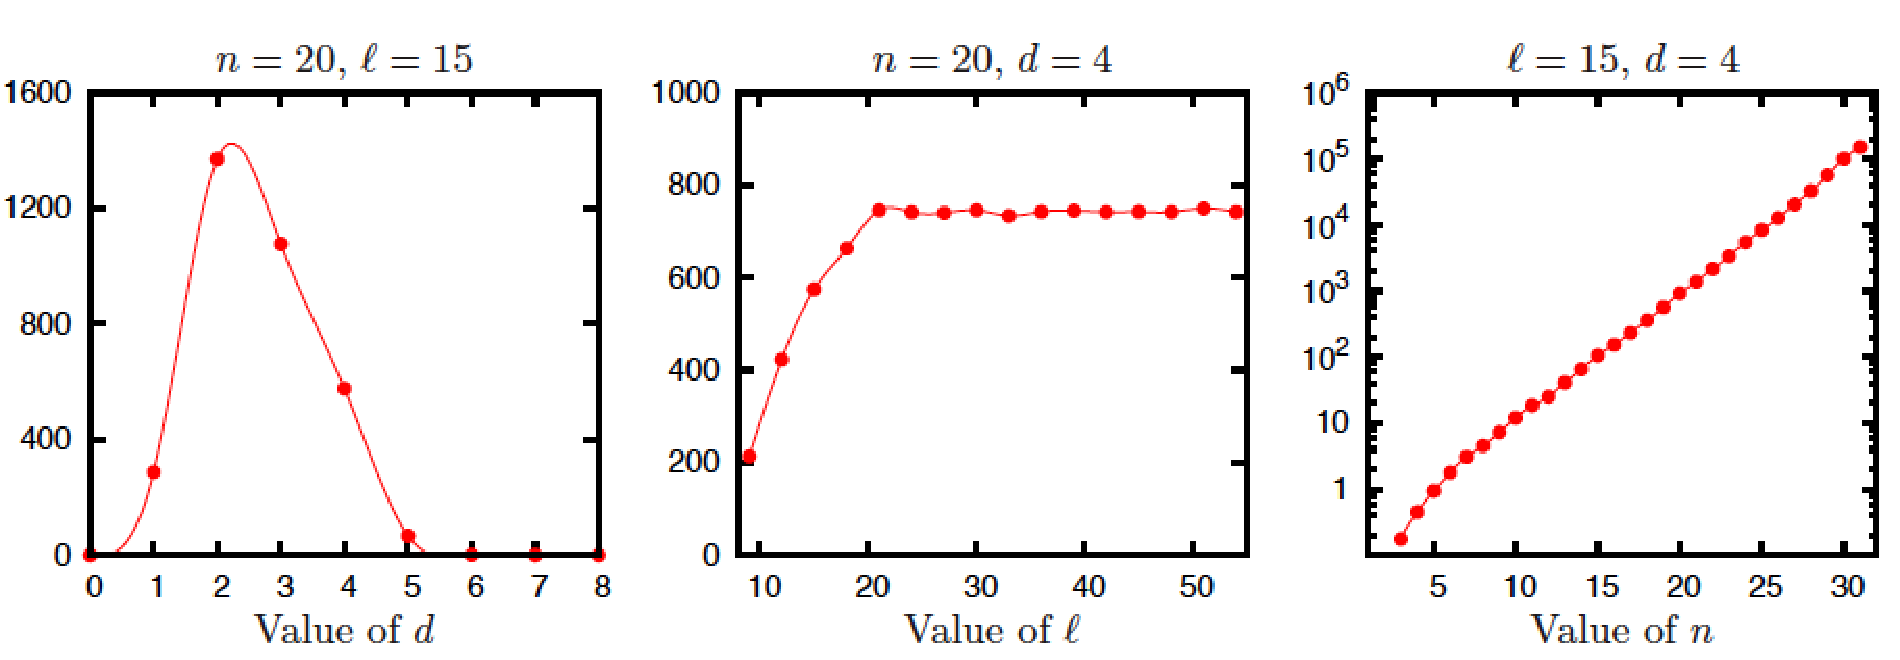
\includegraphics[width=\linewidth]{images/temp}
\caption[Data illustrating the mean number of sets rejected by our rejection sampling heuristic in order to generate a pairwise bounded set.]{Data illustrating the mean number of sets rejected by our rejection sampling heuristic in order to generate a pairwise bounded set. Each plot shows the affect of varying one of the three parameters $n$, $\ell$, and $d$.  Data points are connected with cubic splines.  Note the logarithmic scale used in the right plot.}
\label{fig:separation}
\end{center}
\end{figure}

 The results of the empirical tests are shown in Figure \ref{fig:separation}.  Each of the three plots shows how the average number of rejected sets changes when one of the three parameters is varied and the other two are fixed at their default values.  The left plot shows what happens when $d$ varies between $1$ to $7$.  For values of $d$ that are either greater than $\lfloor \ell /2 \rfloor$ or equal to $0$, any set we generate is pairwise bounded and hence, we did not plot data for $d = 0$ or $d \geq 8$.  The average number of rejected sets is largest when $d$ is equal to 2 and decreases dramatically as $d$ increases. This trend is expected since a large portion of non-pairwise bounded sets would be rejected when $d$ is moderately large.  The middle plot shows what happens when $\ell$ is varied between 9 and 55.  The number of rejected sets increases steadily when $\ell$ varies within the range $[9, 20]$, then plateaus when $\ell$ is above 20.  It can be easily shown analytically that increasing $\ell$ above $2dn$ will have no effect, however, we see empirically that the effect of $\ell$ is minimal for values of $\ell$ greater than 20.  The right plot shows the effect of varying $n$ between $3$ and $31$.  Noting that a logarithmic scale is used, the average number of rejected sets exhibits growth that is clearly exponential in $n$.



%%%%%%%%%%%%%%%%%%%%%%%%%%%%%%%%%%%%%%%%%%%%%%%%%%%%%%%%%%%%%%%%%

\subsection{A Separation of Weight Distributions}

One of the key motivations for the development of methods to generate pairwise bounded sets from an appropriate distribution is that it can be used to determine whether there is a separation between the probability distribution of the weight of a random valid motif set and that of a random decoy set. We use the sampling method just described to generate 1000 random motif sets and 1000 random decoy sets for varying values of $\ell$, $d$, and $n$.  We ran the sampling algorithm described above to generate a pairwise bounded set then determined whether it is a motif set or a decoy set by using the dynamic programming algorithm described in Chapter \ref{chapter:mclwmr}.  We continued generating pairwise bounded sets until we obtained 1000 decoy sets and 1000 motif sets.  For each random motif and decoy set witnessed we calculated the weight of the set.  Figure \ref{fig:separation2} depicts, for values considered for $\ell$, $d$, and $n$, the distribution of the weight of the 1000 random motif sets and that of the 1000 random decoy sets.  The data illustrate an adequate separation between the distributions.  

As the value of $n$ increases, the separation between the distributions becomes more prevalent since the probability distributions become more concentrated around their means and the means themselves diverge.  Further, the dichotomy is again more evident when $(\ell, d)$ is increased from $(15, 4)$ to $(18, 6)$. When $n$ is even moderately large we can use the weight to determine accurately whether the set is a motif set or a decoy set and as $n$ increases this method of using the weight as an indicator will likely increase in accuracy.  Similar conclusions can be made when $\ell$ and $d$ increase. These results suggest that the simple heuristic of using the weight to determine whether a pairwise bounded set is a valid motif set or a decoy set will enable computationally challenging instances of the {\sc Closest String} problem ({\em e.g.}\ when $n \geq 20$ or $(\ell, d)$ is equal to $(18, 6)$) to be solved efficiently with minimal probability of error.


\begin{figure}[h!]
\begin{center} 
 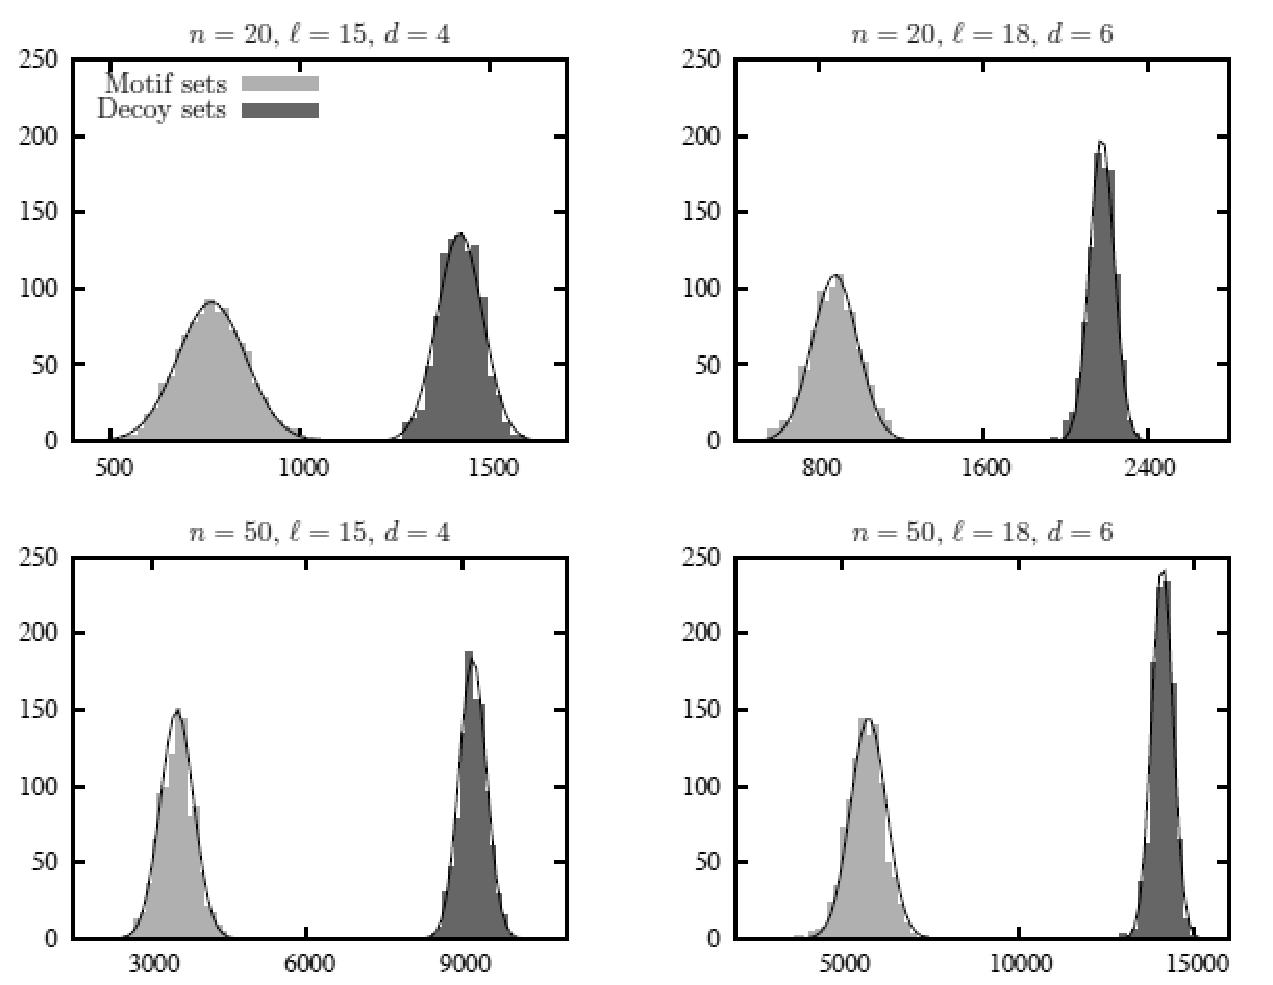
\includegraphics[width=\linewidth]{images/temp2_b_w}
 \caption[Data showing the distribution of the weight of a random motif set, and that of a random decoy set.]{Data showing the distribution of the weight of a random motif set, and that of a random decoy set. Normal distributions fitted to the data are shown to indicate that the weight distributions are approximately normal.}
\label{fig:separation2}
\end{center}
\end{figure}

These empirical trends illustrate the analytical results proved in Chapter \ref{chapter:mclwmr} that demonstrate that the distribution of the weight of a random motif set is tightly concentrated around its mean. It is currently an open problem to prove an analogous result to Theorem \ref{azuma_thm} in Section \ref{section:mcl_wmr_analysis} for an arbitrary decoy set.  This is a considerably more challenging problem due to the lack of a combinatorial characterization of a decoy set.  

%%%%%%%%%%%%%%%%%%%%%%%%%%%%%%%%%%%%%%%%%%%%%%%%%%%%%%%%%%%%%%%%%
\section{An Overview of sMCL-WMR} \label{smcl_wmr_tail_values}

sMCL-WMR considers a weighted graph representation of the input data (as MCL-WMR does), and then uses MCL) \cite{vD00} to cluster the resulting graph. The construction of our graph $\mathcal{G}$ ensures that the motif instances represented by vertices in the graph are connected to each other and form a clique of size $n$, though the converse need not hold. Thus, the problem of finding pairwise bounded sets in the data reduces to finding cliques of size $n$ in the graph $\mathcal{G}$.  Next, we filter out the clusters produced by MCL that do not meet the criteria of having at least $n$ vertices or the minimum weight threshold. See Section \ref{section:mcl_wmr_system} for the details of the construction of the graph and the graph clustering algorithm.  

Figure \ref{fig:separation2} illustrates that both the weight of a random motif set and that of a random decoy set are approximately normally distributed, and shows a separation between these distributions.  Using the rejection sampling method described earlier we calculate the mean and standard deviation of the weight of a random motif set and the weight of a random decoy set. We use $N(\mu, \sigma^2)$ to denote a normal distribution with mean $\mu$ and variance $\sigma^2$.  Let random variables $W_m$ and $W_d$ denote the weight of a random motif set and the weight of a random decoy set, respectively. Let $\mu_m$ and $\sigma_m^2$ respectively denote the mean and variance of the distribution of $W_m$ and similarly, let $\mu_d$ and $\sigma^2_d$ respectively denote the mean and variance of $W_d$.  Assuming that $W_m \sim N(\mu_m, \sigma_m^2)$ and $W_d \sim N(\mu_d, \sigma_d^2)$, we can determine the values $\alpha_m$ and $\alpha_d$ such that: $$\Pr(W_m < \alpha_m) = .99 \mbox{ and } \Pr(W_d > \alpha_d) = .99~.$$ If $\alpha_m < \alpha_d$ then we can use the weight of a pairwise bounded set of strings to determine whether the set is a decoy or a motif as follows: calculate the weight $w$ of the set and, if $w \leq \alpha_m$ or  $w \geq \alpha_d$ then return that the set is a motif or a decoy, respectively; otherwise, use the dynamic-programming algorithm to classify the set.  Hence, if $\alpha_m < \alpha_d$ then more than 99\% of pairwise bounded sets will be classified correctly by considering the weight of the set.  Typically the gap between $\alpha_m$ and $\alpha_d$ is large enough to guarantee that this rate is far higher than 99\%.  In theory it is possible that a set could be misclassified ({\it e.g.}\ if a motif set has weight greater than $\alpha_d$) though in practice the probability of this happening is negligible and does not affect the performance of the algorithm.



\begin{table}[h!]
  \begin{center}
	\begin{tabular}{|c|c|c|c|c|c|c|}
\hline	
$(\ell, d)$& $\mu_m$ & $\mu_d$ & $\sigma_m^2$ & $\sigma_d^2$ & $\alpha_m$ & $\alpha_d$ \\
\hline
\hline
(15, 4)	& 794  		& 1439 	& 84    		& 84    		& 989 		& 1243		 \\
(16, 5) 	& 850 		& 1651 	& 86    		& 102  		& 1050 	& 1413		\\
(18, 6) 	& 899 		& 2204 	& 89    		& 140		& 1106 	& 1878 	 \\
(25, 8)	& 954 		& 2670 	& 111   	& 175  		& 1212 	& 2262		\\
(28, 9)	& 1024 	& 3230 	& 152   	& 199 		& 1378		& 2767		\\
(30, 11)& 1069 	& 3882 	& 169   	& 245 		& 1462		& 3312		 \\
	\hline
	\end{tabular} 
\caption[Data illustrating the mean and standard deviation of the weight of a random motif set and the weight of a random decoy set for various $(\ell, d)$-motif problems.]{Data illustrating the mean and standard deviation of the weight of a random motif set and the weight of a random decoy set for various $(\ell, d)$-motif problems.  The number of strings is fixed at 20.}
\label{chapter6:table3}
\end{center}
\end{table}


\begin{table}[h!]
  \begin{center}
	\begin{tabular}{|c|c|c|c|c|c|c|}
\hline	
$n$ & $\mu_m$ & $\mu_d$ & $\sigma_m^2$ & $\sigma_d^2$ & $\alpha_m$ & $\alpha_d$ \\
\hline
\hline
15 	& 432  	& 980 		& 52  		& 60    	& 552   	& 840  \\
20 	& 794  	& 1439 	& 84  		& 84    	& 989  		& 1243	\\
25 	& 1529 & 2250 	& 129 		& 110	& 1829		& 1994 \\
30 	& 1845 & 3263 	& 196 		& 169  	& 2300 	& 2869\\
35 	& 2240 & 4523 	& 246 		& 213   & 2812 	& 4027 \\
40 	& 3709 & 6110 	& 389 		& 275   & 4613  	& 5460 \\
	\hline
	\end{tabular} 
\caption[Data illustrating the mean and standard deviation of the weight of a random motif set and the weight of a random decoy set for various values of $n$.]{Data illustrating the mean and standard deviation of the weight of a random motif set and the weight of a random decoy set  for various values of $n$. The values $\ell$ and $d$ are fixed at $15$ and $4$, respectively.}
\label{chapter6:table4}
\end{center}
\end{table}

To increase the efficiency of sMCL-WMR, we include a pre-calculated table storing $\mu_m$, $\mu_d$, $\sigma_m^2$ and $\sigma_d^2$ for common values of $\ell$, $d$, and $n$ (for examples see Table \ref{chapter6:table3} and \ref{chapter6:table4}).  We varied $n$ to be between 10 and 50, $\ell$ to be between $15$ and $30$, and $d$ to be between $\lfloor \ell/5\rfloor$ and $\lfloor \ell/2\rfloor$.  Values with weaker motifs or with small data sets ({\em i.e.}\ when $n \leq 10$) are not considered since it was shown that MCL-WMR performs efficiently for these instances. 


%%%%%%%%%%%%%%%%%%%%%%%%%%%%%%%%%%%%%%%%%%%%%%%%%%%%%%%%%%%%%%%%%
\section{An Overview of MCL-FSP}

In many practical applications -- including the analysis of the genetic data in this chapter -- we are not only interested in identifying strings whose maximum distance from each the given strings is minimized but also in identifying strings whose minimum distance from each of the given strings is maximized.  Given a set $S_f$ of strings of length at least $\ell$ over an alphabet $\Sigma$ and a non-negative parameter $d_f$,  the objective of the {\sc Farthest String} problem is to determine if there exists a string $s$ over the alphabet $\Sigma$  such that for any $s_i \in S_f$, $d(s, s_i) \geq d_f$.   We refer to the subsequences occurring in the input sequences as {\em non-motifs}.

We describe a program, {\em MCL-FSP}, that given $n$ length-$m$ sequences over the alphabet $\Sigma$ and parameters $\ell$ and $d$, finds substrings of length $\ell$ in the input data and a length-$\ell$ string $s$ where the goal of the {\sc Farthest String} problem is satisfied with respect to the parameters $\ell$ and $d$.  MCL-FSP can be summarized by the following three steps: graph construction, graph clustering, and recovering the instances and their farthest string.  The graph construction and clustering is similar to MCL-WMR and sMCL-WMR. However, the recovering of the substrings of interest is dramatically different.  The graph constructed for MCL-FSP builds the same set of vertices but joins each pair of vertices by an edge if the Hamming distance between the strings corresponding to the pair of vertices is less than or equal to $d$.  The weight on each edge is $\ell$ minus the Hamming distance between the corresponding strings of the endpoints of the edge.  There exists no additional weighting on the edges. 

The clustering of the graph will yield dense clusters in the graph.  These dense subgraphs will likely contain a set of $n$ substrings that are ``close'' -- meaning the pairwise Hamming distances are small -- and hence, are likely to have a string $s$, which satisfies the {\sc Farthest String} problem together with the set of $n$ substrings.

To recover sets on substrings that satisfy the {\sc Farthest String} problem we first filter out clusters that do not have a substring from each of the input and clusters whose weight is less than $d \cdot {n \choose 2}$. Clusters that pass this test may contain multiple cliques formed by choosing different subsets of $n$ cluster vertices, or possibly no cliques at all. We identify all ways of forming a clique from the cluster vertices by using the $n$-partite nature of the graph to explore all possible cliques with a depth-first search. For each such clique, we use Algorithm \ref{alg:FSP} to determine whether the substrings in the clique correspond to a valid {\sc Farthest String} solution.

\begin{algorithm}[h]
\caption{FSP Recovery Algorithm}
\begin{algorithmic}
\STATE {\bf Input: } A set of $S$ $n$ strings of length $\ell$, parameters $\Delta d$ and $d$, and a candidate string $x$.
\STATE {\bf Output:} A string $s^*$ with the minimum distance to any string in $S$ at least $d$ if it exists and ``Not found'' otherwise.
\STATE If $\Delta d < 0$ then return ``Not found''
\STATE Choose $i \in \{1, \ldots, n\}$ such that $d(x, s_i) < d$. If no such $i$ exists return $x$.
\STATE \hspace{5mm} $\mathcal{P} = \{p \, |  \, x[p] = s_i[p]\}$;
\STATE \hspace{5mm} Choose any $\mathcal{P}'$ from $\mathcal{P}$ with $|\mathcal{P}'| = \ell - d + 1$.
\STATE \hspace{5mm} For each position $p \in \mathcal{P}'$
\STATE \hspace{10mm} Let $x$ not be equal to $s_i$ at position $p$ 
\STATE \hspace{10mm} $s_{ret}$ = FSP Recovery Algorithm ($S$, $\Delta d - 1$, $x$) 
\STATE \hspace{10mm} If $s_{ret} \neq $ ``not found '', then return $s_{ret}$
\STATE Return ``not found''
\end{algorithmic}
\label{alg:FSP}
\end{algorithm}

As mentioned previously, the {\sc Farthest String} problem is NP-complete and therefore, unlikely to be solved in polynomial time. Algorithm \ref{alg:FSP} is based on the bounded search tree algorithm of Gramm {\em et al.}\ \cite{GNR03} for the {\sc Closest String} problem, and has been previously studied by Cheng {\em et al.}\ \cite{cheng}.  Cheng {\em et al.}\ \cite{cheng} proved Algorithm \ref{alg:FSP} has a worst-case running time of $O((|\Sigma|(\ell - d)^{\ell - d})$ and is guaranteed to solve {\sc Farthest String} instances exactly.  

%%%%%%%%%%%%%%%%%%%%%%%%%%%%%%%%%%%%%%%%%%%%%%%%%%%%%%%%%%%%%%%%%

\section{Experimental Results on Synthetic Data}

We tested sMCL-WMR and MCL-FSP on synthetic problem instances generated according to the embedded $(\ell, d)$-motif model, and on real genetic data. The implementations of sMCL-WMR and MCL-FSP are coded in C++, and all experimental tests were performed on a Linux machine with a 64-bit 2600 MHz processor and 1 Gbyte of RAM running Ubuntu.   The running time is given in CPU seconds.  

We follow the experimental methods of Pevzner and Sze \cite{PS00}, and Buhler and Tompa \cite{BT02} by considering the performance of sMCL-WMR and MCL-FSP in comparison to other contemporary and well-known motif-recognition programs on synthetic data.  We fix $n$ to be equal to 20, $m$ to be 600, and consider varied values of $\ell$ and $d$. To produce random motif-recognition instances, we generate a random center string of length $\ell$, then generate $n$ occurrences of the motif, each generated from the center string by randomly choosing $d$ positions and for each of the $d$ positions choosing a random replacement base from the four possible bases (A, C, G, T). We construct $n$ background strings of length $m$ and insert the generated motifs into a random position in the string.  For each of the $(\ell, d)$ combinations, 100 randomly generated sets of input strings were generated. 

We compared the performance of sMCL-WMR and MCL-FSP with that of the following motif-recognition programs: PROJECTION \cite{BT02}, MCL-WMR, PMSprune \cite{JBR07}, and Voting \cite{CL05}.  All programs were run on the same Linux machine with the same data sets.  These motif-recognition programs were chosen for their availability, performance, and widespread use; they are appropriate for comparison with sMCL-WMR because of the previously described capability in solving weak motif instances and because of their availability to be run on the described machine. The results of Voting, PMSprune, and PROJECTION are similar to the ones reported by Davila {\em et al.}\ \cite{JBR07}, and to Chin and Leung \cite{CL06}, both of whose testing was completed on a machine with a slightly slower processor and the same core memory size.  


\begin{table}[h!]
\begin{center} {
	\begin{tabular}{|c|c|c|c|c|c|c|c|}     
    \hline	
	$(\ell, d)$				& sMCL-WMR	 	& MCL-FSP	 	& MCL-WMR		& PROJECTION		& Voting		& PMSprune			\\
	\hline
    (10, 2)					& 122 					& 1131				& 1020 			& 560 (0.98)		& 30				& 42 					\\
	(12, 3)  				& 134 					& 3019				& 2780				& 1921 (0.85) 		& 124			& 130 					\\
	(14, 4)		 			& 492 					& 3325				& 3120				& 3058 (0.88)		& 562			& 556			 		\\
	(16, 5)					& 677 					& 4502				& 4101				& 6132 (0.80)		& 2600		  	& 13121					\\
	(18, 6)					& 1521 				& 8950				& 9202				& -						& 8023			& 29012  				\\
	(20, 7)					& 2845					& -					& -					& -						& 24600		& - 						\\
	(25, 8)				    & 4111 				& -					&	-					& -						&	-			 	& - 						\\
%	(28, 10)				& 2791 				& -					&	-					& -						&	-			   	& - 						\\
	\hline
	\end{tabular}}
\end{center}
\caption[Comparison of the performance of sMCL-WMR, MCL-FSP, and other motif-recognition programs on synthetic data for various values of $\ell$ and $d$.]{Comparison of the performance of sMCL-WMR, MCL-FSP, and other motif-recognition programs on synthetic data for various values of $\ell$ and $d$. All programs except PROJECTION had a success rate of 1.0 and for this reason, the success rate was for PROJECTION is included in brackets in the table. In all experiments, $m = 1000$ and $n = 20$.}
\label{smcl_wmr:compare1}
\end{table}


\begin{table}[h!]
\begin{center} {
	\begin{tabular}{|c|c|c|c|c|c|c|}     
	\hline	
	$n$			& sMCL-WMR	& MCL-FSP		& MCL-WMR		& PROJECTION		& Voting				& PMSprune\\
	\hline
    18			& 547 				& 5559				& 5320				&	5230 (0.85)		& 3930					& 37020 \\
	20  			& 679				& 8823				& 8912				&  -						& 5201					& 45030  \\
	24		  	& 1221 			& -					& -					&	-						& 10211				& - \\
	28			& 2019				& -					& -					&	-						&	-						& - \\
	30			& 2431		 		& -					& -					&	-						&	-						& - \\
	40			& 5201		 		& -					& -					&	-						&	-						& - \\
	\hline
	\end{tabular}}
	\end{center}
	\caption[Comparison of the performance of sMCL-WMR, MCL-FSP, and other motif-recognition programs on synthetic data for various values of $n$.]{Comparison of the performance of sMCL-WMR, MCL-FSP, and other motif-recognition programs on synthetic data for various values of $n$. All programs except PROJECTION had a success rate of 1.0 and for this reason, the success rate was for PROJECTION is included in brackets in the table.In all experiments, $\ell = 18$, $d = 6$ and $m = 1000$.}
\label{smcl_wmr:compare2}
\end{table}
	

Tables \ref{smcl_wmr:compare1} and \ref{smcl_wmr:compare2} illustrate the comparison between the running time of sMCL-WMR and that of the other programs.  Our aim was to test the selected programs on their capability to solve challenging motif instances ({\em i.e.}\ when $d$ is significantly large with respect to $\ell$).  The symbol ``-'' implies that the program was not capable of solving the motif instance on the described machine in a reasonable amount of time, which we define to be at most 20 hours, or with reasonable accuracy, which we define to be at least 75\%.  Two significant trends are witnessed in the data: sMCL-WMR is capable of solving very hard instances of motif recognition ({\em i.e.}\ when $\ell = 25$ and $d = 8$) and gives a dramatic improvement over the existing programs for instances where $\ell \geq 16$ (for instances where $\ell \leq 12$ sMCL-WMR had comparable or better performance to the other programs). MCL-FSP had a slightly higher running time than MCL-WMR and failed on the same instances as MCL-WMR. 


\section{Development of a Seed Coat-Specific Promoter for Canola}

Canola ({\em Brassica napus L.}) was originally bred from rapeseed in Canada in the 1970s \cite{downey}. Presently, the canola industry generates more than \$11 billion of yearly income to the Canadian economy. One of the major exports of the canola industry is {\em canola meal}, which is most widely used in animal feeds. However, one of the major problems with canola meal is the dark polyphenolic pigments that accumulate in the seed coat; the dark pigment interferes with the protein utilization, causing the quality of the meal to be lowered. Hence, altering the seed coat is an important biological challenge that has the possibility of reducing the indigestible fiber and enhancing the usability of canola meal.  One first step in  tackling this problem is to develop seed coat-specific promoters which are capable of regulating the genes involved in seed coat development and metabolism. 

One approach to finding seed coat-specific promoters for canola is to isolate the promoters of proved seed coat-specific genes from other species, and then validate their expression in canola.  Since genes are conserved among species, this is a reasonable approach.  Preliminary results identified that several promoters express in the outer integument of seed coat in canola, and a single promoter expresses in the inner integument. The subsequent challenge is to synthetically develop a promoter sequence that expresses both these two biological characteristics.  This synthetic promoter can then be artificially inserted into the genomes of the canola seeds and be tested for their expression. Table \ref{table:promoters} gives an overview of the relevant data concerning the promoter sequences analyzed.      
     
\begin{table}[h!]
\begin{center} {
\begin{tabular}{|l|c|cccc|}     
\hline	
Promoter		& bp		& \multicolumn{4}{c|}{Composition} \\		
					&						& A 			& C 			& G 			& T \\
\hline
\hline
 AtLAC15 		&1528 				& 33\%  	& 19\%  	& 16\% 	& 33\% \\
\hline
Arabidopsis BAN & 236 		& 33\%  	& 18\%  	 & 14\%  	& 34\% \\
\hline
VPE				& 2067 			& 34\%  	& 16\%  	& 17\%  	& 32\% \\
\hline
GILT 			& 2889 			& 36\%  	& 13\%  	& 14\%  	& 37\% \\
\hline
Arabidopsis TT12 & 1704	& 36\%  	&16\%  	& 17\%  	& 31\%\\
\hline
Arabidopsis TT2  & 3813 	& 38\%  	& 14\%   	& 14\%  	& 34\% \\
\hline
Barley Germin B gene & 846 & 35\% 	& 15\%		& 15\%		& 35\%\\
\hline
Tobacco Cryptic       & 2553 & 33\%  	& 18\%  	 & 14\%  	& 34\% \\
\hline
SCS1							& 7235 & 37\%  	& 12\% 	& 12\%  	& 39\% \\
\hline
SCB1 						& 5329	& 38\%		& 12\%		& 15\%		& 35\\ 
\hline
	\end{tabular}}
	\end{center}
	\caption[Description of promoters analyzed to develop a coat-specific promoter.]{Description of promoters analyzed to develop a coat-specific promoter.}
\label{table:promoters}
\end{table}


In order to use sMCL-WMR to find motifs in the genetic data we need to ensure that there exists a separation between the weight of the motif sets and decoy sets found in the data.  We have previously shown such a separation exists for synthetic data.  For a subset of the values of $n$, $\ell$ and $d$ that are to be used in the analysis, we ran MCL-WMR and calculated the weight of the motif sets and decoy sets found.  Figure \ref{fig:canola_separation} illustrates this data. For all values of $n$, $\ell$, and $d$ tested, there exists a clear separation between the distributions and we were able to use the precalculated tail values determined in Section \ref{smcl_wmr_tail_values}.

\begin{figure}[h!]
\centering
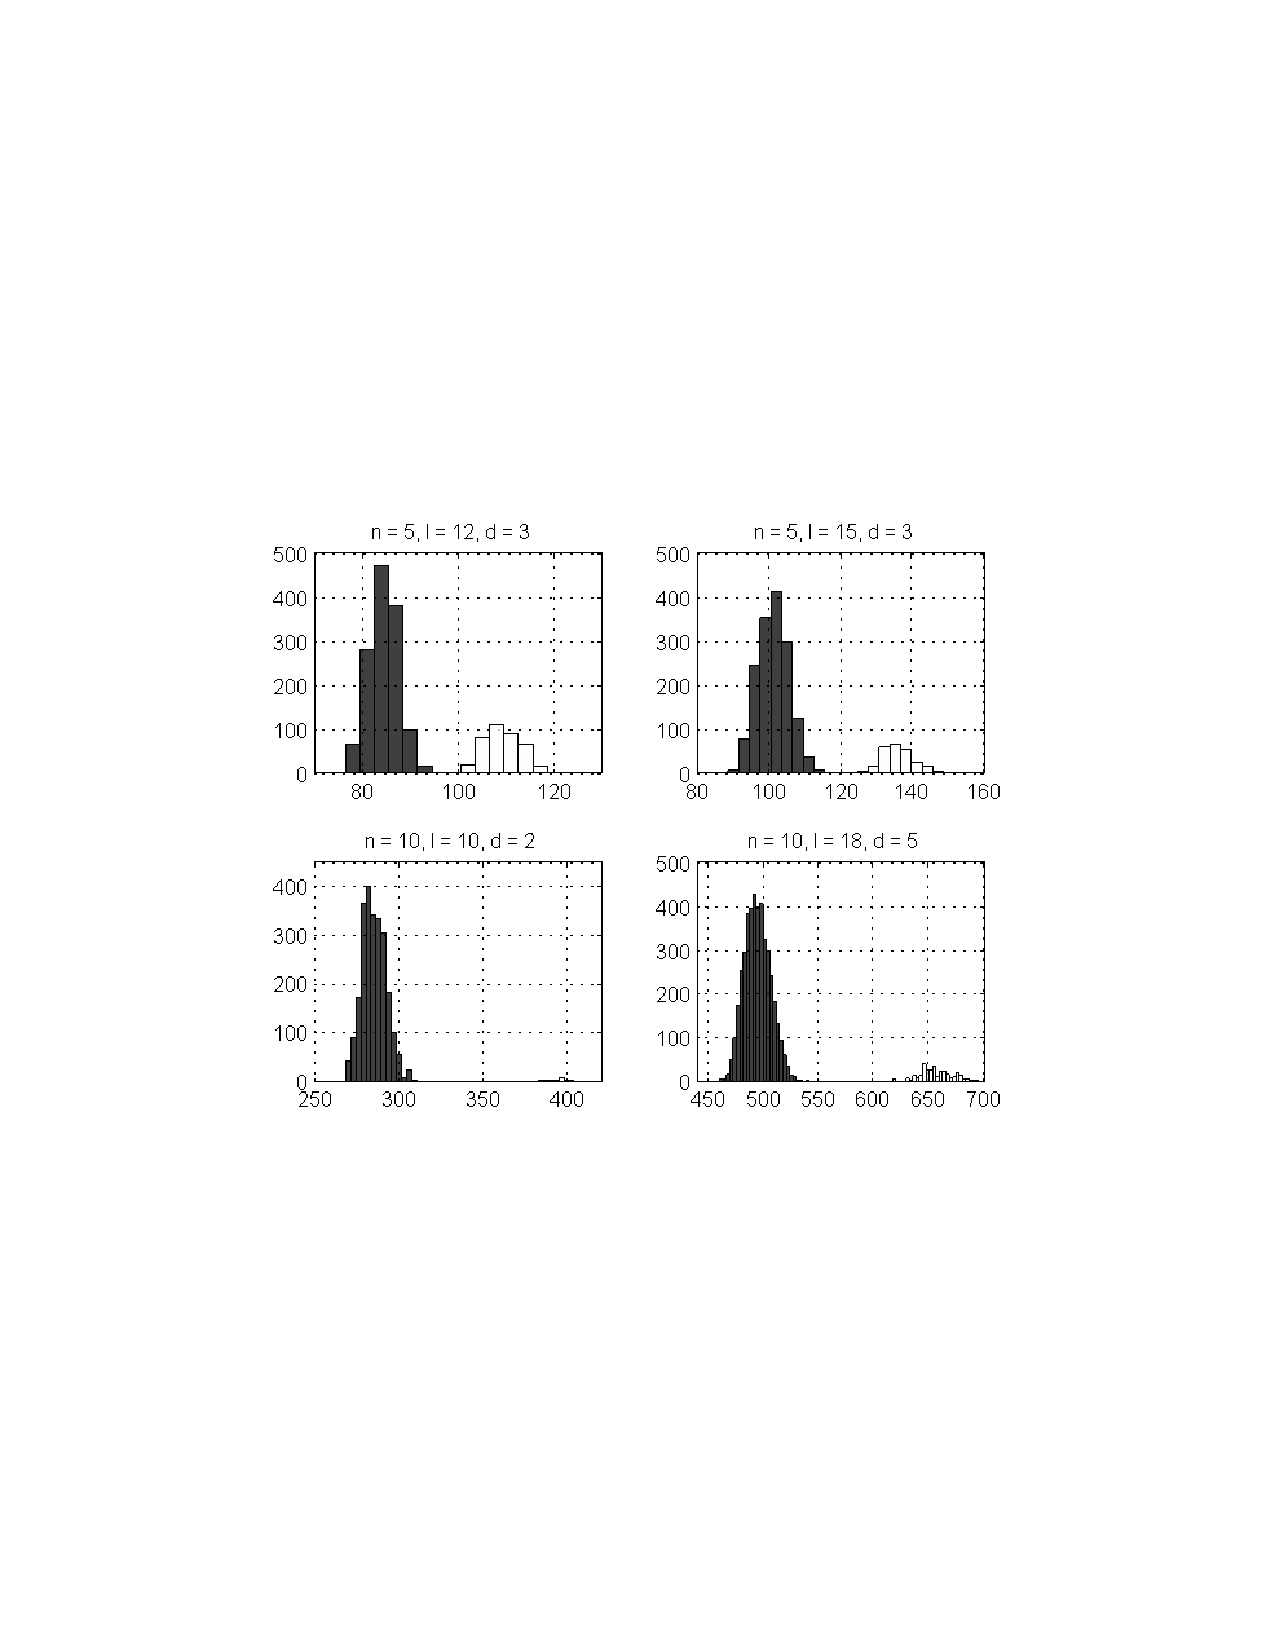
\includegraphics[width=90mm,trim=7cm 8cm 7cm 7cm]{images/canola_separation}% picture filename
 \caption[An Illustration of the distribution of the weight of a random motif set found in the promoter data, and that of a random decoy set found in the promoter data.]{An Illustration of the distribution of the weight of a random motif set found in the promoter data (shown in white), and that of a random decoy set found in the promoter data (shown in black). }
\label{fig:canola_separation}
\end{figure}


The conserved motifs were identified through the use of sMCL-WMR and MCL-FSP. Table \ref{table:detected_motifs} gives a subset of the motifs detected by sMCL-WMR and the CPU time in seconds for their detection.  In addition, it was of interest to identify furthest strings that were contained in one of the input sequences.  Table \ref{table:detected_nonmotifs} contains a sample of the furthest strings and which of the input sequences it occurs in; for the remaining sequences the specified string is a furthest string with respect to the parameters $\ell$ and $d$.  In particular, detecting furthest strings that occurred in one of the following three promoters was of interest: the AtLAC15, Arabidopsis BAN and Arabidopsis TT2 promoters.  

Each of these promoters has a specific biological role in the development of one of the different layers of seed coat. sMCL-WMR was used to determine the nucleotide patterns common to each of the promoters and hence, maybe responsible for having biological activity concerning the seed-coat. MCL-FSP was used to detect nucleotide patterns that were distinct to particular promoters that were responsible for the outer integument and inner integument of the seed coat -- in hope of identifying biological sequence patterns responsible for each specific seed-coat integument.  We identified more than 40 motifs and non-motifs in the promoter data that may be responsible for the seed coat-specificity. 

Based on these motifs and non-motifs, a promoter DNA sequence of approximately 700 bp was synthesized and introduced into canola.  Presently laboratory tests are being used to obtain the complete expression results.
     

\begin{table}[h!]
\begin{center} {
\begin{tabular}{|c|c|c|c|}     
\hline	
$(\ell, d)$ & $n$ 		& Center String		& CPU time \\		
\hline
\hline
$(6, 1)$	& 10 									& ACActc					& 58 \\
$(6, 2)$	& 10 									& tGgtCA					& 63 \\
$(9, 1)$	&	9 										& taTCTttTT				& 98 \\
$(9, 2)$	&	7 										& TTgtTAGgt			& 96 \\
$(10, 2)$	&	8 										& TTTTtTattT			& 112 \\
$(12, 3)$	&	10 									& tcTCTTtttCta			& 198 \\
$(14, 4)$	&	7 									 	& AgtTctATTtttTT			& 253 \\
 \hline
	\end{tabular}}
	\end{center}
	\caption[Subset of motifs detected using sMCL-WMR.]{Subset of motifs detected using sMCL-WMR. The CPU time is in seconds.}
\label{table:detected_motifs}
\end{table}

\begin{table}[h!]
\begin{center} {
\begin{tabular}{|c|c|c|c|}     
\hline	
$(\ell, d)$ & Occurrence 		& Furthest String		& CPU time \\		
\hline
\hline
$(10,4)$	& AtLAC15			& ACCACTCCAG						& 1025 \\
$(18, 8)$	& AtLAC15			& GATTTCCAAGCCTATCAC		& 1128 \\
$(19, 9)$ 	& AtLAC15			& CCAAGAATCGATGAGCGGG	& 2591 \\
$(15, 6)$	& Arabidopsis BAN & GATCTACTGTTGTAC			& 1891 \\
$(17, 7)$  & Arabidopsis BAN & ATCACGTGCTTACCTTC		& 2139 \\
$(15,7)$	& Arabidopsis TT2 & CCGACGGGTTTGGCT 			& 1811 \\
$(18,9)$ 	& Arabidopsis TT2 & CAGCGAAAAGGCCGACGG	& 2350\\
 \hline
	\end{tabular}}
	\end{center}
	\caption[Subset of motifs detected using MCL-FSP.]{Subset of motifs detected using MCL-FSP. The CPU time is in seconds.}
\label{table:detected_nonmotifs}
\end{table}



\section{Summary and Open Problems}

We investigated the relationship between the weight of a decoy set and the weight of a motif set by means of random sampling. We discussed a rejection sampling strategy, and proposed a means to make this uniform sampling method more efficient. Using this algorithm that generates pairwise bounded sets uniformly at random, we studied the probability distributions of the respective weights of a random motif set and a random decoy set.  We concluded that the weight of a pairwise bounded set can accurately predict whether the set is a valid motif set.  We illustrated how to exploit this dichotomy to create a more efficient motif-recognition program.  

Developing a more efficient method to generate pairwise bounded sets uniformly at random is an important algorithmic challenge that would give insight into the motif-recognition problem. Studying the possibility of the use of Markov chain Monte Carlo (MCMC) sampling algorithms to sample pairwise bounded sets warrants further investigation; such methods have led to efficient sampling algorithms for other combinatorial problems; see Randall \cite{randall} for a survey of MCMC methods and their applications.  Further, an analytical explanation for the empirical results, showing that almost all decoy sets with degeneracy parameter $d$ have center strings when the degeneracy allowed is increased to $d + 2$, would lead to a more efficient sampling method and would be interesting in its own right.

In addition, we developed and applied an efficient algorithm for the {\sc Furthest String} problem.  This problem is significantly less investigated than its partner problem, the {\sc Closest String} problem, and as such, it warrants more in-depth study. 

\chapter{Conclusions}
\label{sec:conclusions}

%\section{Future Work}
%\label{sec:future-work}

%----------------------------------------------------------------------
% END MATERIAL
%----------------------------------------------------------------------

% B I B L I O G R A P H Y
% -----------------------

% The following statement selects the style to use for references.  It controls the sort order of the entries in the bibliography and also the formatting for the in-text labels.
\bibliographystyle{plain}
% This specifies the location of the file containing the bibliographic information.  
% It assumes you're using BibTeX (if not, why not?).
\bibliography{uw-ethesis}
% The following statement causes the title "References" to be used for the biliography section:
\renewcommand{\bibname}{Bibliography}
\addcontentsline{toc}{chapter}{\textbf{Bibliography}}
% Tip 5: You can create multiple .bib files to organize your references. 
% Just list them all in the \bibliogaphy command, separated by commas (no spaces).

% The following statement causes the specified references to be added to the bibliography% even if they were not 
% cited in the text. The asterisk is a wildcard that causes all entries in the bibliographic database to be included (optional).
\nocite{*}

\end{document}
